\documentclass[11pt]{article}
\usepackage[a4paper,margin=18mm]{geometry}
\usepackage[no-math]{fontspec}
\setmainfont{Latin Modern Roman}
\usepackage{amsmath,amssymb,amsthm,xfrac,xspace,hyperref,graphicx,comment}
\excludecomment{DefTralics}
\providecommand{\backmatter}{}
\providecommand{\loccit}{\emph{loc. cit.}}

\providecommand{\bibliofont}{\small}
\newcommand{\ie}{i.e.,\xspace}
\newcommand{\eg}{e.g.,\xspace}
\newcommand{\etc}{etc.\xspace}
\newcommand{\cf}{cf.\xspace}
\newcommand{\resp}{resp.\xspace}
\newcommand{\smaller}{\small}
\newcommand{\Subsection}{\subsection}
\newcommand{\Subsubsection}{\subsubsection}
\newcommand{\skpt}{\smallskip}
\emergencystretch=3em
\numberwithin{equation}{section}
% Begin literal retained input author-preamble.tex
\usepackage[scr=rsfs,cal=euler]{mathalfa}
\usepackage[all,cmtip]{xy}\let\labelstyle\textstyle

\multlinegap0pt
\newcommand{\Psfrac}[2]{(\sfrac{#1}{#2})}
\newcommand{\psfrac}[2]{\sfrac{(#1)}{#2}}
\newcommand{\spfrac}[2]{\sfrac{#1}{(#2)}}
\newcommand{\pspfrac}[2]{\sfrac{(#1)}{(#2)}}
\newcommand{\RedefinitSymbole}[1]{%
\expandafter\let\csname old\string#1\endcsname=#1
\let#1=\relax
\newcommand{#1}{\csname old\string#1\endcsname\,}%
}
\RedefinitSymbole{\forall} \RedefinitSymbole{\exists}

\newcommand\mto{\mathchoice{\longmapsto}{\mapsto}{\mapsto}{\mapsto}}
\newcommand\hto{\mathrel{\lhook\joinrel\to}}
\newcommand{\quand}{\quad\text{and}\quad}


% Literal retained local macro units
% Native source immediately aliases sole nicefrac use to its sfrac.


\usepackage{mathtools}

\let\nicefrac\sfrac

\usepackage{tikz}
\usetikzlibrary{matrix,arrows,arrows.meta,calc,intersections}
\tikzset{>={Stealth[width=1.5mm,length=1.5mm]}}
\usepackage{tikz-cd}

\newtheorem{theorem}{Theorem}[subsection]
\newtheorem{lemma}[theorem]{Lemma}
\newtheorem{corollary}[theorem]{Corollary}
\newtheorem{proposition}[theorem]{Proposition}
\newtheorem{statement}[theorem]{Statement}
\newtheorem{conjecture}[theorem]{Conjecture}
\newtheorem{claim}[theorem]{Claim}

\theoremstyle{remark}
\newtheorem{definition}[theorem]{Definition}
\newtheorem{remark}[theorem]{Remark}
\newtheorem{motivation}[theorem]{Motivation}
\newtheorem{observation}[theorem]{Observation}
\newtheorem{justification}[theorem]{Justification}
\newtheorem{warning}[theorem]{Warning}
\newtheorem{question}[theorem]{Question}

\let\mc\mathcal
\let\ms\mathscr
\let\mb\mathbb
\let\df\emph

\let\eps\varepsilon
\let\phi\varphi

\newcommand{\compl}[1]{{{#1}^{\text{c}}}}

\newcommand{\vv}{{\vvv}}
\DeclareMathOperator{\vvv}{v}

\DeclareMathOperator{\sign}{sign}
\DeclareMathOperator{\wei}{wt}
\DeclareMathOperator{\realo}{PsG}
\DeclareMathOperator{\dist}{dist}
\DeclareMathOperator{\pg}{PsG}
\DeclareMathOperator{\pog}{Ps\widetilde G}
\DeclareMathOperator{\pe}{PsE}
\DeclareMathOperator{\g}{G}
\DeclareMathOperator{\oG}{\widetilde G}
\DeclareMathOperator{\e}{E}
\let\oe\relax
\DeclareMathOperator{\oe}{\widetilde E}
\DeclareMathOperator{\poe}{Ps\widetilde{E}}
\DeclareMathOperator{\pgproj}{\pi_{\pg}}
\DeclareMathOperator{\gproj}{\pi_{\g}}
\DeclareMathOperator{\pogproj}{\pi_{\pog}}
\DeclareMathOperator{\oGproj}{\pi_{\oG}}
\DeclareMathOperator{\orth}{O}
\DeclareMathOperator{\sorth}{SO}
\DeclareMathOperator{\stief}{V}
\DeclareMathOperator{\pstief}{PsV}
\DeclareMathOperator{\sphere}{S}

\DeclareMathOperator{\cell}{cell}
\DeclareMathOperator{\Cell}{\overline{cell}}
\DeclareMathOperator{\conf}{conf}
\DeclareMathOperator{\upto}{until}

\newcommand{\Rpol}[1]{\mb{R}\mathrlap{{}^{#1}}{}_\text{pol}}
\DeclareMathOperator{\pol}{pol}
\DeclareMathOperator{\aim}{aim}

\newcommand{\Ball}{\text{\rm Ball}}
\DeclareMathOperator{\proj}{proj}
\DeclareMathOperator{\stereo}{stereo}
\DeclareMathOperator{\interp}{interp}
\DeclareMathOperator{\coord}{coord}
\DeclareMathOperator{\ho}{ho}
\DeclareMathOperator{\id}{id}

\DeclareMathOperator{\cov}{cov}
\DeclareMathOperator{\omg}{om_G}
\DeclareMathOperator{\ompsg}{om_{PsG}}
\DeclareMathOperator{\ot}{ot}
\DeclareMathOperator{\mcp}{MacP}

\DeclareMathOperator{\curves}{PsL}

\DeclareMathOperator{\cyl}{cyl}

\newcommand{\projplane}{\mb{RP}^2}


% End literal retained input author-preamble.tex

\begin{document}
\begin{center}{\Large Stable item 2061}\end{center}
\paragraph{Source and attribution.}
Michael Gene Dobbins, \emph{Grassmannians and pseudosphere arrangements}, Journal de l’École polytechnique — Mathématiques 8 (2021), publisher version, DOI 10.5802/jep.171. \href{https://jep.centre-mersenne.org/articles/10.5802/jep.171/}{Publisher article}. Authors' text: \href{https://creativecommons.org/licenses/by/4.0/}{CC BY 4.0}.
\paragraph{Editorial problem boundary.}
Prove only the finite rank-three chirotope part of Theorem2.7.1 below restricted to the unit-weight realization subspace: each nonloop pseudocircle has weight1 and loops have weight0. Use the exact author weighted-Fréchet topology and quotient by orientation-preserving isometries \(SO(3)\). All new continuous canonical coordinates, equivariant Kneser modification and cellwise interpolation/boundary-continuity proofs are retained. The deformation acts through sphere homeomorphisms and preserves these fixed weights. Arbitrarily varying weights, the unoriented quotient, infinite arrangements and the global Stiefel/Grassmannian deformation theorem are outside this selected claim.
\paragraph{Difficulty (editorial): H2.}
The cited topological representation and Kneser theorems do not produce a continuous deformation on the oriented realization quotient. The author builds continuous canonical coordinates, modifies Kneser's deformation to respect precomposition by isometries, and proves that cellwise conformal interpolation depends continuously on pseudocircle boundaries. These compatibility arguments make the final quotient contraction well defined on the fixed unit-weight finite chirotope subspace.
\paragraph{Editorial transcription note.}
Original author language, mathematics and ordering are preserved. Publisher front matter is replaced by this independent article wrapper. Bibliography is recovered from matching cached publisher HTML, including its TeX formulas. No new proof or mathematical repair is supplied. Surrounding original results are retained for conservative context and are not extra selected corpus claims.
\clearpage

% Begin literal retained input author-body.tex
\section{Introduction}

If we record all the possible ways a given vector configuration or affine point set can be partitioned by a hyperplane, the resulting combinatorial data will be an oriented matroid \cite{bjorner1999oriented}.
From this data, we can determine such information as, what points appear on the boundary of the convex hull of a point set, the faces of the resulting polytope, the solutions to a linear programming optimization problem, whether polytopes intersect, and the visibility between points around or on the boundary of a polytope.
Understanding the necessary properties of this data can be used for proving theorems and developing algorithms for finite point sets in Euclidean space \cite{oswin2013,cardinal2019subquadratic,DobHolHub2014Erdos,habert2012,knuth1992axioms,novick1,novick2,shnurnikov2016tk}.

Oriented matroids are more general objects, however, since not all oriented matroids arise from a vector configuration. Indeed, it is ETR-complete, which is at least NP-hard, to determine whether a given oriented matroid can be realized by a vector configuration \cite{shor1991stretchability}.
In contrast, the topological representation theorem says that every oriented matroid can be realized by a pseudosphere arrangement \cite{folkman1978oriented}.

\begin{figure}[htb]
\begin{center}

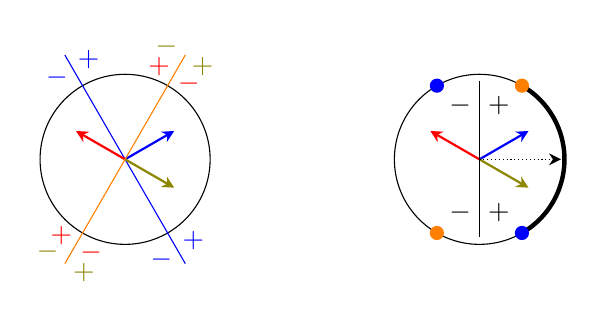
\begin{tikzpicture}[scale=.9]

\begin{scope}[shift={(-5cm,0)}]

\draw
(0,0) circle (1.2)
;

\draw[thick,->,blue]
(0,0) -- (30:0.8)
;

\draw[blue]
(-60:1.7) -- (120:1.7)
(-50:1.5) node {$+$} (110:1.5) node {$+$}
(-70:1.5) node {$-$} (-230:1.5) node {$-$}
;

\draw[thick,->,red]
(0,0) -- (150:0.8)
;

\draw[thick,->,olive]
(0,0) -- (150:-0.8)
;

\draw[red]
(70:1.4) node {$+$} (230:1.4) node {$+$}
(50:1.4) node {$-$} (250:1.4) node {$-$}
;

\draw[olive]
(70:1.7) node {$-$} (230:1.7) node {$-$}
(50:1.7) node {$+$} (250:1.7) node {$+$}
;

\draw[orange]
(60:1.7) -- (240:1.7)
;

\end{scope}

\draw
(0,0) circle (1.2)
;

\draw[thick,->,blue]
(0,0) -- (30:0.8)
;

\draw[thick,->,red]
(0,0) -- (150:0.8)
;

\draw[thick,->,olive]
(0,0) -- (150:-0.8)
;

\draw[ultra thick]
(-60:1.2) arc (-60:60:1.2)
;

\fill[blue]
(-60:1.2) circle (.1)
(120:1.2) circle (.1)
;

\fill[orange]
(60:1.2) circle (.1)
(240:1.2) circle (.1)
;

\draw
(110:.8) node {$-$} (-110:.8) node {$-$}
(70:.8) node {$+$} (-70:.8) node {$+$}
;
\draw
(90:1.1) -- (-90:1.1)
;
\draw[densely dotted,->]
(0,0) -- (1.15,0)
;

\end{tikzpicture}
\end{center}

\caption{Left: a vector configuration in the plane with the associated subdivision of the unit circle.
Right: a cell in the subdivision of the circle with the associated partition of the vectors.}
\label{figure-sign-covectors}

\end{figure}

\begin{figure}[htb]
\begin{center}

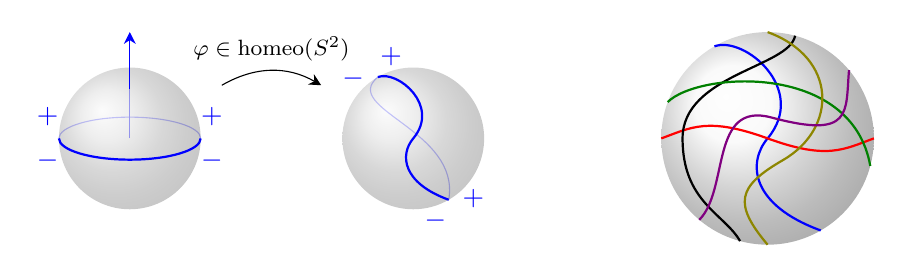
\begin{tikzpicture}[scale=.9]

\begin{scope}[rotate = 0]
\draw[blue!30]
(1,0) arc (0:180:1 and .3)
;\end{scope}

\draw[blue!50]
(0,0) -- (90:.7)
;

\shade[ball color=black!30, white, opacity=.3]
circle (1)
;

\draw[blue,->]
(90:.7) -- (90:1.5)
;

\begin{scope}[rotate = 0]
\draw[thick,blue]
(1,0) arc (0:-180:1 and .3)
;\end{scope}

\draw[blue]
(15:1.2) node {$+$} (-15:-1.2) node {$+$}
(-15:1.2) node {$-$} (15:-1.2) node {$-$}
;

\path (30:1.5) coordinate (a);

\begin{scope}[shift={(4cm,0cm)}]

\draw[blue!30]
(-60:1) .. controls +(80:1) and +(220:.7) .. (120:1)
;

\shade[ball color=black!30, white, opacity=.3]
circle (1)
;

\draw[thick,blue]
(-60:1) .. controls +(160:.7) and +(50:-.3) ..
(0,0) .. controls +(50:.6) and +(20:.3) .. (120:1)
;

\draw[blue]
(-45:1.2) node {$+$} (105:1.2) node {$+$}
(-75:1.2) node {$-$} (-225:1.2) node {$-$}
;

\path (-30:-1.5) coordinate (b);

\end{scope}

\path[->]
(a) edge[bend left] node[auto] {\footnotesize $\varphi \in \text{homeo}(S^2)$} (b)
;

\begin{scope}[shift={(9cm,0cm)},scale=1.5]

\shade[ball color=black!5, white, opacity=.5]
circle (1)
;

\draw[thick,blue]
(-60:1) .. controls +(160:.7) and +(50:-.3) ..
(0,0) .. controls +(50:.6) and +(20:.3) .. (120:1)
;

\draw[thick,red]
(0:1) .. controls +(200:.3) and +(-20:.6) ..
(0,0) .. controls +(-20:-.6) and +(20:.3) .. (0:-1)
;

\draw[thick]
(75:1) .. controls +(260:.3) and +(90:.6) ..
(0:-.8) .. controls +(90:-.6) and +(120:.3) .. (75:-1)
;

\draw[thick,green!50!black]
(-20:-1) .. controls +(45:.4) and +(100:1) .. (-15:1)
;

\draw[thick,olive]
(270:1) .. controls +(130:.5) and +(210:.5) ..
(-55:.25) .. controls +(210:-.6) and +(-20:.7) .. (90:1)
;

\draw[thick,violet]
(40:1) .. controls +(85:-.4) and +(-15:.8) ..
(80:.2) .. controls +(-15:-.6) and +(45:.4) .. (50:-1)
;

\end{scope}

\end{tikzpicture}
\end{center}

\caption{Left: a vector with the associated great circle and the pseudocircle obtained as its homeomorphic image.
Right: a pseudocircle arrangement.}
\label{figure-pseudosphere}

\end{figure}

A pseudosphere arrangement is a topological analog to data representing the direction of each vector in a vector configuration.
More precisely, given a vector configuration in $\mb{R}^k$, we can define a hyperplane arrangement by associating each vector to its orthogonal complement. From this hyperplane arrangement, we can define a sphere arrangement by intersecting each hyperplane with the unit sphere. In this way, the direction of each non-zero vector is represented by an oriented great $(k{-}2)$-sphere in the $(k{-}1)$-sphere.
This defines a subdivision of the sphere, and each cell of this subdivision corresponds to a way of partitioning the given vector configuration by a hyperplane; see Figure \ref{figure-sign-covectors}. This is one way to obtain an oriented matroid.
In contrast, a pseudosphere arrangement is a collection of oriented topological embeddings of $(k{-}2)$-spheres in the $(k{-}1)$-sphere satisfying certain conditions given in Section~\ref{subsection-pseudosphere}, and the cells of a pseudosphere arrangement define an oriented matroid; see Figure \ref{figure-pseudosphere}. Moreover, every oriented matroid can be obtained in this way.
In this paper we deal with weighted pseudosphere arrangements, where each pseudosphere gets a weight analogous to the norm of a vector.

The hardness of deciding whether a given oriented matroid can be realized by a vector configuration is a consequence of Mnëv's universality theorem, which says that for any semialgebraic set $X$, there is a rank $3$ oriented matroid $\mc{M}$, such that the quotient by isometry of the subspace of vector configurations realizing $\mc{M}$ has the homotopy type of $X$ \cite{mnev1988universality}.
In other words, if you were hoping for the set of vector configurations that can be partitioned by a hyperplane in a certain fixed set of ways to define a `nice' topological space, then you may be disappointed to know that such a space can be as horrible as any space that you can define algebraically.
The topological representation theorem may be understood as saying that the space of realizations by pseudosphere arrangements is always at least non-empty.
Here we take this farther by showing that in contrast to Mnëv's theorem, the space of realizations by pseudosphere arrangements is always contractible up to isometry in rank 3; see Theorem~\ref{theorem-pseudoreal-contract}.\footnote{This is actually proved for weighted pseudosphere arrangements, but here the weights play no role.}

We also consider the space of \emph{all} $n$-element rank $k$ weighted pseudosphere arrangements, which we call the pseudolinear Stiefel manifold $\pstief_{k,n}$.
One way to define the real Stiefel manifold $\stief_{k,n}$ is as the space of all $n \times k$ matrices with orthonormal columns, or equivalently up to diffeomorphism, as the space of all spanning configurations of $n$ vectors in $\mathbb{R}^k$ considered up to symmetric positive definite linear transformation.
In rank 3, we show that each pseudolinear Stiefel manifold is homotopy equivalent to the corresponding real Stiefel manifold, $\pstief_{3,n} \simeq \stief_{3,n}$.
Moreover, there is a natural embedding of $\stief_{3,n}$ in $\pstief_{3,n}$, and we provide a strong deformation retraction from $\pstief_{3,n}$ to $\stief_{3,n}$ that is equivariant with respect to the orthogonal group~$\orth_3$; see Theorem \ref{theorem-grassman-pseudograssman}.
This holds even in the case where $n = \infty$.
We also consider the quotient of the pseudolinear Stiefel manifold by the orthogonal and special orthogonal groups, which we call the pseudolinear Grassmannians and oriented pseudolinear Grassmannians. We show that these are homotopy equivalent to the corresponding real Grassmannians and oriented Grassmannians.
That is, we have the homotopy equivalences,
\begin{align*}
\g_{3,n} &= \stief_{3,n} / \orth_k \simeq \pg_{3,n} = \pstief_{3,n} / \orth_k, \\
\oG_{3,n} &= \stief_{3,n} / \sorth_3 \simeq \pog_{3,n} = \pstief_{3,n} / \sorth_3.
\end{align*}
This means that weighted pseudosphere arrangements effectively have the same global topology as vector configurations in rank 3.

These homotopy equivalences motivate the association of weights to pseudosphere arrangements.
As a vector configuration moves along on a path through a Stiefel manifold, some of the vectors may pass through the origin. For a weighted pseudosphere arrangement, this would correspond to a pseudosphere vanishing from the arrangement and then reappearing somewhere else. Since this must happen continuously, we include weights that go to zero as a pseudosphere vanishes.

One source of interest in Grassmannians is as classifying spaces for vector bundles.
Recall that a real rank $k$ vector bundle is a space that locally has the structure of a product of $\mb{R}^k$ with a space $B$, called the base space; for a precise definition see \cite[p.\,24]{husemoller1994fibre}.
The infinite Grassmannian $\g_{k,\infty}$ is a classifying space for rank $k$ vector bundles in the following sense.
Every rank $k$ vector bundle with base space $B$ can be defined up to isomorphism by a map from $B$ to $\g_{k,\infty}$, and two maps define isomorphic vector bundles if and only if the maps are homotopy equivalent, provided that~$B$ is paracompact.
We show that the infinite pseudolinear Grassmannian $\pg_{3,\infty}$ is a classifying space for rank $3$ vector bundles, the infinite oriented pseudolinear Grassmannian $\pog_{3,\infty}$ is a classifying space for rank $3$ oriented vector bundles, and the pseudolinear Stiefel manifold is universal for $\orth_3$ fiber bundles; see Corollary~\ref{corollary-classifying}.

Oriented matroids have a natural partial order, and the MacPhersonian $\mcp_{k,n}$ is the poset of all rank $k$ oriented matroids on $n$ elements.
Nicolai Mnëv and Günter Ziegler conjectured that the polyhedral chain complex of the MacPhersonian $\mcp_{k,n}$ is homotopy equivalent to the corresponding real Grassmannian $\g_{k,n}$, as part of a more general conjecture \cite{mnev1993combinatorial}.
The question of whether a more general class of posets called OM-Grassmannians are homotopy equivalent to the corresponding real Grassmannians
arose from the work of Israel Gelfand and Robert MacPherson on computing Pontrjagin classes using oriented matroids \cite{gelfand1992combinatorial}.
Mnëv and Jürgen Richter-Gebert showed that the answer is no in general by exhibiting a OM-Grassmannian that is not homotopy equivalent to the corresponding real Grassmannian \cite{mnev1993two}, while
Mnëv and Ziegler conjectured that the homotopy equivalence still holds for a more restricted class, namely the OM-Grassmannians of realizable oriented matroids \cite{mnev1993combinatorial}.
This conjecture of Mnëv and Ziegler was recently
disproved by Gaku Liu \cite{liu2020counterexample}.
However, the special case of the conjecture for the MacPhersonian, which we will call the MacPhersonian conjecture, remains open.
Mnëv and Ziegler had anticipated that a proof of the rank $3$ case of the MacPhersonian conjecture would appear in Eric Babson's Ph.D.\ thesis, but no such proof appeared \cite{mnev1993combinatorial,babson1993combinatorial}.
An erroneous proof of the MacPhersonian conjecture was prominently published and has subsequently been retracted \cite{biss2003homotopy,biss2009erratum}.
If true, this conjecture would provide a representation of the homotopy type of the Grassmannian as a simplicial complex defined by purely combinatorial conditions.
Another important consequence of the MacPhersonian conjecture is that we could represent a vector bundle over a simplicial complex as a poset map to the MacPhersonian in a way that gives a bijection between isomorphism classes of vector bundles and matroid bundles \cite{anderson2002mod,anderson1999matroid}.
The present paper does not deal with the MacPhersonian, but may be regarded intuitively as evidence for this conjecture, particularly in rank~$3$.

In the face of Mnëv's universality theorem, the MacPhersonian conjecture may seem overly optimistic for two reasons.
First, we have a natural map $\omg$ from the Grassmannian $\g_{3,n}$ to the MacPhersonian $\mcp_{3,n}$ sending each vector configuration to its associated oriented matroid,
but this map is not surjective. Second, the preimage $\omg^{-1}(\mc{M})$ of an oriented matroid $\mc{M}$ can have the homotopy type of any primary semialgebraic set, even in rank 3.
That is, the Grassmannian may be decomposed into realizations of oriented matroids, but the resulting pieces have highly complicated topology, as do their intersections.
The conjecture would suggest that we can simply ignore the topology of these pieces and that of their intersections, and this will have no bearing on the topology of the Grassmannian as a whole.
The MacPhersonian conjecture may already seem intuitively more reasonable in light of Theorem \ref{theorem-pseudoreal-contract} and Theorem \ref{theorem-grassman-pseudograssman}. These theorems say that $\omg$ factors into maps $\iota$ and $\ompsg$ through the pseudolinear Grassmannian $\pg_{3,n}$ such that the following diagram commutes,
\[
\xymatrix{
& \pg_{3,n}\ar[dr]^-\ompsg & \\
\g_{3,n}\ar[ur]^-\iota\ar[rr]^-{\omg} & & \mcp_{3,n} \\
}
\]
the map $\iota$ is a homotopy equivalence, the map $\ompsg$ is surjective, and for every rank $3$ oriented matroid $\mc{M} \in \mcp_{3,n}$, the preimage $\ompsg^{-1}(\mc{M}) \subset \pg_{3,n}$ is contractible.
This is the first stage of a project to prove the rank $3$ case of the MacPhersonian conjecture; it remains to show that $\pg_{3,n}$ and $\mcp_{3,n}$ are homotopy equivalent.

In higher rank, other obstacles may raise doubt on generalizing these results. For example, the proofs of the main results here use the fact that the quotient by isometries of the space of self homeomorphisms of the $2$-sphere is contractible \cite{kneser1926deformationssatze}, which may fail in higher dimensions \cite[\S 10.12]{kirby1977foundational}.
Also, extension spaces of higher rank oriented matroids can be disconnected, even in the realizable case \cite{liu2020counterexample}.
On the other hand, the fact that universality holds for realizations of oriented matroids even when restricted to rank $3$ indicates that rank $3$ is a crucial case.

Several ideas used in this paper were developed based
on discussions with Laura Anderson and
on the author's prior work with Andreas Holmsen and Alfredo Hubard on generalizing Mnëv's universality theorem to arrangements of convex sets in the plane \cite{dobbins2017realization}, which in turn stemmed from work generalizing the Erdős-Szekeres theorem from point sets to arrangements of convex sets \cite{DobHolHub2014Erdos,dobbins2017realization}.

\subsubsection*{Organization}

In Section \ref{section-def} we develop the technical details needed to define the main objects of the paper, which are the pseudolinear Grassmannians, defined in Section \ref{subsection-psg-def}, and to formally state the main theorems in Section \ref{subsection-main-theorems}.
Some definitions that are not required to state the main theorems are put off to later sections.
In Section \ref{section-contractible}, we prove the first main theorem, which says that the space of pseudocircle arrangements representing a fixed rank $3$ oriented matroid is contractible.
In Section \ref{section-deforming}, we prove the second main theorem, which says that each pseudolinear Grassmannian is homotopy equivalent to the corresponding real Grassmannian in rank 3.
This uses an explicit strong deformation retraction from the space of weighted pseudocircle arrangements to the space of weighted great circle arrangements.
In Section \ref{section-bundles}, we prove the main corollary, which says that the infinite rank $3$ pseudolinear Grassmannian is a classifying space for rank $3$ vector bundles.

We use \df{Claim} for statements that are only meaningful in the context where they appear, and claims can depend on variables set to certain values in that context. In contrast, we use \df{Lemma} for statements that stand on their own.

\subsubsection*{Acknowledgments}

The author would like to thank
Laura Anderson,
Pavle Blagojević,
Kenneth Clarkson,
Xavier Goaoc,
Andreas Holmsen,
and Alfredo Hubard
for helpful discussions and insights.
The author would also like to thank the anonymous referees for many helpful comments which significantly improved the readability.
Part of this work was done at the 2019 IBS summer research program on Algorithms and Complexity in Discrete Structures, hosted by the IBS discrete mathematics group.

\section{Main definitions and theorems}\label{section-def}

\subsection{Basic notation}

Here we briefly give some basic notation which is mostly standard, but may not be universally consistent in the literature. If the reader should encounter unfamiliar notation, it might be found in this subsection. More substantive definitions appear in later subsections.

We use round brackets
$(x_1,\dots,x_n) \in X^n$ to denote a sequence and curly brackets $\{x_1,\dots,x_n\} \subset X$ to denote a set.
To append an entry $y$ to a sequence $I = (x_1,\dots,x_n)$, we write $I \cdot y = (x_1,\dots,x_{n},y)$.
We may abuse notation by writing $x\in I$ to denote that $x$ appears in the sequence $I$, as well as set membership.
We use the notation $[n]_{\mb{N}} = \{1,\dots,n\}$ and $[a,b]_{\mb{R}} = \{x \in \mb{R} : a \leq x \leq b\}$,
with round brackets for strict inequalities.
The unit sphere in $\mb{R}^k$ is denoted by $\sphere^{k-1} = \left\{ x\in \mb{R}^k : \|x\|^2 = 1 \right\}$, and the closed unit ball by $\Ball^k$.
We call the intersection of a pointed convex cone in $\mb{R}^k$ with the sphere $\sphere^{k-1}$, a convex subset of the sphere, or we say a spherically convex set for emphasis.
For a convex subset $C$ of the sphere or the projective plane and points $x_i \in C$, we use $[x_1,\dots,x_n]_C$ to denote the polygonal path in $C$ with vertices $x_1,\dots,x_n$ in that order and geodesic edges. Note that this is not defined when $x_i,x_{i+1}$ are antipodal.

We denote the set of all homeomorphisms from a space $X$ to a space $Y$ by
$\hom(X,Y)$,
and $\hom(X) = \hom(X,X)$.
Let $\hom^+(\sphere^d)$ be
the component of $\hom(\sphere^d)$ that contains the identity map,
\ie positively oriented reparameterizations of the sphere.
$\orth_k$ denotes the orthogonal group of rank $k$, which we may regard as the subgroup of isometries in $\hom(\sphere^{k-1})$ or as a set of ($k\times k$)-matrices when convenient, and $\sorth_k$ denotes the special orthogonal group.
We will generally treat linear operators and matrices interchangeably.
We denote the adjoint operator or transpose matrix of~$A$ by $A^*$.	

We use $x \mto \varphi$ for the function defined by substituting a value for $x$ into a formula $\varphi$.
We may separate arguments of a function by `;' for emphasis when partial application will be used. That is, given a function $f : X \times Y \to Z$, we denote by $f(c) : Y \to Z$ the function $y \mto f(c;y)$.
A partial function is a function that is defined on some subset of $X$ and is denoted by $f:X \not\to Y$.

\subsection{Grassmannians}\label{subsec-vectconfig}

Here we begin developing background needed to formally state the main theorems. We start with the global topology of vector configurations.
Let $X$ be a $k$ dimensional real vector space with an inner product $\langle,\rangle$, an orthonormal basis $e_1,\dots,e_k$, and unit sphere $\sphere(X) = \{u \in X: \|u\|=1\}$. For the time being, we~could regard $X$ to be $\mb{R}^k$, but we will mostly work in the vector space $X = \Rpol{k}$ defined later.

A vector configuration $(a_1,\dots,a_n)$ spanning a vector space $X$ is a \df{Parseval frame} when any of the following equivalent conditions are satisfied:

\vbox{
\begin{itemize}
\item
For all $u \in \sphere(X)$, $\langle a_1,u \rangle^2 + \dots +\langle a_n,u \rangle^2 = 1$.
\item
For all $x \in X$, $\langle a_1,x \rangle^2 + \dots +\langle a_n,x \rangle^2 = \|x\|^2$.
\item
The linear map $x \mto (\langle a_1,x\rangle,\dots,\langle a_n,x\rangle)$ from $X$ to $\mb{R}^n$ is an isometry.
\item
The $(n\times k)$-matrix $A$ with $a_i$ in the $i$-th row has orthonormal columns.
\end{itemize}
}

The Stiefel manifold and Grassmannian can be defined in several ways that are equivalent up to homeomorphism. Here, we define the \df{Stiefel manifold}
\[
\stief_{k,n} = \stief_{k,n}(X)\quad\text{for }k \leq n \in \mb{N}
\]
to be the space of Parseval frames of $X$ indexed by $[n]_\mb{N}$.
We define the \df{Grassmannian} as the quotient by the orthogonal group $\g_{k,n} = \stief_{k,n}/\orth_k$
and the \df{oriented Grassmannian} as the quotient by the special orthogonal group $\oG_{k,n} = \stief_{k,n}/\sorth_{k}$.
We define a metric on $\stief_{k,n}$ for $n$ finite as follows. For $A = (a_1,\dots,a_n)$ and $B = (b_1,\dots,b_n) $, let
\[ \dist(A,B) = \max \{ \|a_i - b_i\| :i \in [n]_\mb{N} \}. \]
This induces a metric on $\g_{k,n} = \stief_{k,n}/\orth_k $ that is defined for $\mc{A},\mc{B} \in \g_{k,n}$ by
\[ \dist(\mc{A},\mc{B}) = \inf\{ \dist(A,B) : A \in \mc{A}, B \in \mc{B} \}. \]

\begin{observation}
Since $\g_{k,n}$ and $\oG_{k,n}$ are defined as the quotient of $\stief_{k,n}$ by a group of isometries, $\dist$ is a metric, and the metric topology is the same as the quotient topology for $n$ finite.
\end{observation}

\begin{justification}
Why do we define the Grassmannian using row vectors of a matrix?
There are various equivalent ways the Grassmannian could be defined, depen\-ding on how a point in the Grassmannian is represented, and likewise for the Stiefel manifold.
A point in $\stief_{k,n}$ is commonly represented as an orthonormal sequence of $k$ vectors in $\mb{R}^n$, \ie the columns of the matrix $A$ in the last definition of a Parseval frame.
Likewise, a point in $\g_{k,n}$ may alternatively be represented as a $k$-dimensional vector subspace of $\mb{R}^n$, \ie the column space of the matrix $A$.
For us it is more convenient to consider the rows of $A$ rather than the columns so that later we will be able to extend these spaces of vector configurations to larger spaces defined by weighted pseudospheres.
We choose to represent the elements of our vector configuration as row vectors of $A$ so that the orthogonal group $\orth_k$ acts on the right. Later $\orth_k$ will act by precomposition as a subspace of $\hom(\sphere^2)$, which makes this choice consistent with the traditions that composition is written right to left and matrix multiplication on the right acts on rows.
\end{justification}

\begin{justification}
Why do we use Parseval frames?
A central theme of this paper is the global topology of vector configurations, which the Grassmannian is meant to encompass.
The Grassmannian can alternatively be defined as the quotient by general linear transformations $\mathrm{GL}(\mb{R}^k)$ of the space of all spanning vector configurations. This definition may have greater appeal as the global space of vector configurations, but the result is homeomorphic to our definition of the Grassmannian, which has the advantage of a metric that is more straightforward to define, because we quotient by $\orth_k$. This will be important later when we extend this metric to the pseudolinear Grassmannian.
The subgroup $\orth_k \subset \mathrm{GL}(\mb{R}^k)$ has a greater abundance of smaller orbits in the space of vector configurations, so to keep the same quotient space while quotienting by a subgroup, we must restrict to fewer orbits.
Each orbit of $\mathrm{GL}(\mb{R}^k)$ contains exactly one orbit of $\orth_k$ consisting of Parseval frames, which is one reason for restricting spanning vector configurations to Parseval frames.
\end{justification}

We identify a Parseval frame that ends with a tail of zeros with the shorter frame where the trailing zero are removed so that $\stief_{k,k} \subset \stief_{k,k+1} \subset \stief_{k,k+2} \subset \cdots$,
and we define the infinite Stiefel manifold as the union of this ascending chain of spaces,
\[ \stief_{k,\infty} = \bigcup_{n=k}^\infty \stief_{k,n}. \]
Similarly, we define the infinite Grassmannian $\g_{k,\infty}$ and oriented Grassmannian $\oG_{k,\infty}$ as the corresponding quotients of $\stief_{k,\infty}$, which are also unions of ascending chains of Grassmannians.

On the infinite Stiefel manifold and infinite (oriented) Grassmannian, we use the direct limit topology, which is the finest topology such that the inclusion maps \hbox{$\stief_{k,n} \hto \stief_{k,\infty}$} are continuous.
Equivalently, this topology is defined by the universal property that a function $\phi : \stief_{k,\infty} \to Y$ to any topological space $Y$ is continuous if and only if the restriction of $\phi$ to $\stief_{k,n}$ is continuous for all $n$.

\begin{warning}
It may be tempting to use the metric on $\stief_{k,\infty}$ defined in the same way as the metric we use on $\stief_{k,n}$ for $n<\infty$, but the resulting metric topology differs from the topology we use here.
For example, consider the sequence
\[A_i = (e_1,e_2,\tfrac{i-1}{i}\,e_3,\underbrace{0,\dots,0}_i,\tfrac{1}{i}\,e_3,0,\dots) \in \stief_{3,\infty}. \]
The distance from $A_i$ to $(e_1,e_2,e_3,0,\dots)$ vanishes, but $A_i$ does not converge in the direct limit topology.
Notice that it is easier for a function to be continuous in the direct limit topology, and harder for limits to converge, because it is so fine.
\end{warning}

\subsection{Combinatorial data from vector configurations}\label{subsection-combinatorial-data}

Here we extract combinatorial data from vector configurations.
We represent a vector $a \in \mb{R}^k$ by the pair $\pol(a) = (\|a\|,\aim (a))$ where
\[ \aim (a) : \sphere^{k-1} \to \{+,0,-\}, \quad \aim (a; x) = \sign \langle a,x \rangle.\]
This is effectively the polar form of $a$ where the direction of $a$ is represented by $\aim(a)$.
We call the elements of $\{+,0,-\}^n$ \df{sign sequences}.
For a vector configuration $A = (a_1,\dots,a_n) \in (\mb{R}^k)^n$ and $x \in \mb{R}^k$, let
\begin{align*}
\aim (A;x) &= (\aim(a_1;x),\dots,\aim(a_n;x)) \in \{+,0,-\}^n, \\
\cov (A) &= \bigl\{ \aim (A; v) :v \in \sphere^{k-1} \bigr\} \subseteq \{+,0,-\}^n.
\end{align*}
That is, $\cov(A)$ consists of the sign sequence corresponding to each cell in the subdivision of the sphere $\sphere^{k-1}$ by the arrangement of hyperplanes with normal vectors $a_1,\dots,a_n$.
Equivalently, $\cov(A)$ consists of all the ways $A$ can be partitioned by a hyper\-plane.
We call $\cov(A)$ the \df{sign covector sphere} of~$A$.
Note that $\cov(A)$ captures equivalent data about~$A$ as the oriented matroid of $A$ and may be thought of and referred to informally as the oriented matroid of $A$.

The \df{order type} of a vector configuration $A = (a_1,\dots,a_n) \in (\mb{R}^k)^n$ is the function
\[ \ot(A): [n]_\mb{N}^k \to \{+,0,-\}, \quad \ot(A;i_1,\dots,i_k) = \sign\det(a_{i_1},\dots,a_{i_n}). \]
The order type tells us which subsets of vectors form a basis, and in each case, the orientation of that basis.
Observe that the order type of a configuration is invariant under special linear transformations, while the sign covector sphere is invariant under general linear transformations.
Note also that the sign covector sphere of a configuration is determined by its order type. On the other hand, if the sign covector sphere is given, then there are two possibilities for the order type.

Since we are interested in the above combinatorial information about vector configurations, it will be more convenient for us to work with vectors that are already in polar form. To that end, we define a vector space of vectors in polar form.
We denote by $\Rpol{k} = \pol(\mb{R}^k)$ the vector space isomorphic to $\mb{R}^k$ by $\pol$ inheriting the usual scalar multiplication, vector addition, inner product, norm, standard basis vectors, and the action of matrices as linear transformations. Note that we do not have a nice formula for adding vectors $a,b \in \Rpol{k}$, other than $a+b = \pol(\pol^{-1}(a)+\pol^{-1}(b))$.

We abuse notation by letting $e_i$ denote the $i$-th standard basis vector of $\Rpol{k}$ or~$\mb{R}^k$ for each $k$ as convenient.
We let $i^+$ denote the sign sequence with $(+)$ in the $i$-th place and $0$ elsewhere,
$i^-$ denote the sign sequence with $(-)$ in the $i$-th place and $0$ elsewhere.

\subsection{Chirotopes and oriented matroids}\label{subsection-chirotopes}

Chirotopes are similar to the order type of a vector configuration, but take as axioms certain necessary conditions for a sign-valued function to be the order type of some vector configuration. Theorems and algorithms involving vector configurations often depend only on these necessary conditions, and as such, can be generalized to chirotopes.
Reformulating geometric algorithms in terms of chirotopes provides a clearer understanding of how the algorithms work and how basic geometric properties are being used.
We will not make use of these axioms directly, but instead make use of the rich literature of lemmas and theorems that have been built on them.
Later we will give a second equivalent definition of chirotopes.
While the axiomatic definition may be more elegant and simpler to state, the second definition will be more relevant when we get to the geometric constructions in later sections.

Firstly, a sign-valued function on $[n]_\mb{N}^k$ is defined to be a \df{chirotope} of \df{rank} $k$ when it satisfies the following axioms.

\vbox{\begin{enumerate}
\item $\chi$ is not the constant function 0.
\item For all permutations $\pi$, $\chi(i_{\pi(1)},\dots,i_{\pi(k)}) = \sign(\pi) \chi(i_1,\dots,i_k)$.
\item For all $i_1,\dots,i_k,j_1,\dots,j_k$, there is an $h$ such that
\[\chi(i_1,\dots,i_k)\chi(j_1,\dots,j_k) \in \{ 0,\chi(j_h,i_2,\dots,i_k)\chi(j_1,\dots,j_{h-1},i_1,j_{h+1},\dots,j_k) \}.\]
\end{enumerate}}
The order type of a vector configuration is always a chirotope, and the intuition and motivation behind these axioms can be understood from what they say about vector configurations.
Namely, the first condition says that every spanning vector configuration has a basis.
The second condition says that if we form a square row matrix and then permute the rows, then the sign of the determinant of the matrix changes according the the sign of the permutation of the rows.
The third condition says that the signed basis exchange principle from linear algebra holds.
This says that if we have two ordered bases $v_1,\dots,v_k$ and $u_1,\dots,u_k$ with the same orientation, then we can always find some vector $u_h$ of one basis such that if we swap that vector with the first vector $v_1$ of the other basis, then we get two ordered bases $u_h,v_2,\dots,v_k$ and $u_1,\dots,u_{h-1},v_1,u_{h+1},\dots,u_k$ that again have the same orientation, and likewise with oppositely oriented bases.

A \df{basis} of a chirotope is a set $\{i_1,\dots,i_k\}$ such that $\chi(i_1,\dots,i_k) \neq 0$.
A subset of~$[n]_\mb{N}$ is \df{independent} when it is a subset of a basis.
Note that this defines a matroid, but we will not deal with general matroids here.

The \df{\hbox{$\stief$-realization} space} of a rank $k$ chirotope $\chi$ is
\[ \stief(\chi) =
\{ A \in \stief_{k,n}:\ot (A) = \chi\},
\]
and the \df{$\oG$-realization space} is
\[ \oG(\chi) = \stief(\chi)/\sorth_k \subset \oG_{k,n}. \]

Oriented matroids are another combinatorial abstraction of vector configurations like chirotopes.
There are several equivalent sets of data that can be used to define oriented matroids, and which of these is most convenient can vary depending on context and purpose.
For us, oriented matroids are primitive objects, \ie objects that are not composed of other objects unlike sets or sequences. For example, integers are typically regarded as primitive objects.
We treat oriented matroids as primitive objects as a way to encapsulate the data used to define oriented matroids in a way that is ecumenical toward the peculiarities of each of the various ways that data can be represented.

We give several equivalent definitions of oriented matroids.
Firstly, \df{oriented matroids} are defined to be primitive objects that correspond bijectively to pairs of chirotopes related by a reversal of sign, \ie a pair of the form $\{\chi,-\chi\}$.
Equivalently, oriented matroids can be defined as primitive objects corresponding bijectively to sets of sign sequences satisfying certain axioms, which are necessary conditions for the set to be the sign covector sphere of a vector configuration \cite[\S 3.7]{bjorner1999oriented}.
These axioms, which we will not list, have a similar flavor to the chirotope axioms.
For each oriented matroid $\mc{M}$, we call the corresponding set of sign sequences the \df{sign covector sphere} of~$\mc{M}$ and denote it by $\cov(\mc{M})$.
Note this is also called the set of non-zero sign covectors of~$\mc{M}$.
The rank, bases, and independent sets of an oriented matroid are defined to be the same as those of the corresponding chirotopes.

The \df{\hbox{$\stief$-realization} space} of a rank $k$ oriented matroid $\mc{M}$ is
\[ \stief(\mc{M}) =
\{ A \in \stief_{k,n}:\cov (A) = \cov(\mc{M})\},
\]
and the \df{$\g$-realization space} is
\[ \g(\mc{M}) = \stief(\mc{M})/\orth_k \subset \g_{k,n}. \]

\subsection{Weighted pseudosphere arrangements}\label{subsection-pseudosphere}

As mentioned in the introduction, many important geometric properties of a configuration $A$ can be determined from $\cov(A)$ or $\ot(A)$.
However, some disadvantages of working with this data are that deciding whether a given oriented matroid can be realized by a vector configuration is algorithmically intractable and does not admit a combinatorial characterization \cite{shor1991stretchability,vamos1978missing,mayhew2018yes}. Furthermore, even for realizable oriented matroids, the realization space can be highly complex topologically.
Here we define an extension of $\Rpol{k}$ where these disadvantages are mitigated.

A rank $k$ oriented \df{pseudosphere} is a map $\theta : \sphere^{k-1} \to \{+,0,-\}$ such that there is some orientation preserving self-homeomorphism $\phi \in \hom^+(\sphere^{k-1})$ such that \hbox{$\theta \circ \phi = \aim (e_k)$}; see Figure \ref{figure-pseudosphere}.
We may simply call $\theta$ a pseudosphere, with the understanding that it is oriented and has some rank.
Pseudospheres on $\sphere^2$ are called \df{pseudocircles}.

A \emph{non-trivial} \df{weighted pseudosphere} is a pair $\alpha = (r,\theta)$ consisting of a positive real number $r>0$ and a pseudosphere $\theta$. Additionally, there is the \emph{trivial} weighted pseudosphere $0 =\pol(0) = (0,\, x \mto 0)$, which is the origin of $\Rpol{k}$.
We let
\[\|\alpha\| = r \quad \text{ and } \quad \aim (\alpha) = \theta.\]
We denote the kernel of $\alpha$ (or $\theta$) by $S_\alpha = S_\theta = \theta^{-1}(0)$.
We can scale weighted pseudospheres by $s \in \mb{R}$ by $s \alpha = (|s|r,\sign(s)\theta)$ for $s\neq 0$ and $0\alpha = 0$.
However, we~cannot add weighted pseudospheres in general.

A \df{pseudosphere arrangement} is a sequence of pseudospheres $\Theta = (\theta_1,\dots,\theta_n)$ that satisfies the following.
For all $I \subseteq [n]_\mb{N}$,
$S_I = \bigcap_{i \in I} S_{\theta_i} $ is either empty or a topological sphere, meaning there is a homeomorphism $\phi_I : \sphere^{k_I} \to S_I$ for some $k_I \leq k$,
and if~$S_I$ is non-empty then $(\theta_1 \circ \phi_I,\dots, \theta_n \circ \phi_I)$ is again a pseudosphere arrangement; see Figure \ref{figure-pseudosphere}.
Pseudosphere arrangements were introduced by Jim Lawrence to provide a model for oriented matroids \cite{folkman1978oriented}.

A \df{weighted pseudosphere arrangement} is a sequence of rank $k$ weighted pseudospheres ${A} = (\alpha_1,\dots,\alpha_n)$ such that $(\aim(\alpha_1),\dots,\aim(\alpha_n))$ is a pseudosphere arrangement.
We may simply write $S_i = S_{\{i\}} = S_{\theta_i}$.
We say $A$ and $\Theta$ are \df{spanning} when $S_{1} \cap \dots \cap S_{n} = \emptyset$. In other words, for every $x \in \sphere^{k-1}$, there is some $\alpha_i$ that does not vanish at $x$.

For $J \subseteq [n]_\mb{N}$, let $\proj_J(A) = (\beta_1,\dots,\beta_n)$ where
\[\beta_i =
\begin{cases} \alpha_i & i\in J, \\ 0 & i \not\in J .\end{cases} \]

We can extract combinatorial data from weighted pseudosphere arrangements analogous to the data extracted from vector configurations.
For a weighted pseudosphere arrangement $A = (\alpha_1,\dots,\alpha_n)$,
we let
\begin{align*}
\wei(A) &= (\|\alpha_1\|,\dots,\|\alpha_n\|) \in \mb{R}^n, \\
\aim (A) &= \aim(\alpha_1)\times \dots\times \aim(\alpha_n) : \mb{R}^k \to \{+,0,-\}^n, \\
\cov (A) &= \bigl\{ \aim (A; v) :v \in \sphere^{k} \bigr\} \subseteq \{+,0,-\}^n.
\end{align*}
We call $\cov (A)$ the \df{sign covector sphere} of $A$.
We also define $\aim$ and $\cov$ analogously for pseudosphere arrangements without weights.
For $\sigma \in \cov (A)$, let
\[ \cell(A,\sigma) = \bigl\{u \in \sphere^{k-1}:\aim (A; u) = \sigma \bigr\}, \]
and let $\Cell(A,\sigma)$ be the closure of $\cell(A,\sigma)$.

\begin{remark}\label{remark-cell}
Mandel showed that the subdivision of $\sphere^{k-1}$ by a pseudosphere arrangement is a regular cell decomposition \cite{edmonds1978topology}.
\end{remark}

We order the set of sign sequences $\{+,0,-\}^n$ by the product of the relation $(\leq_\vv)$ where ${0 <_\vv ({+})}$, and ${0 <_\vv ({-})}$, and the pair $({+}),({-})$ are incomparable.
This ordering corresponds to the inclusion ordering on the subdivision of the sphere by a pseudosphere arrangement. That is, $\Cell(A,\sigma) \subseteq \Cell(A,\tau)$ if and only if $\sigma \leq_\vv \tau$ for all $\sigma,\tau \in \cov(A)$.
The sign covector sphere is always a graded poset with this ordering,
and the height of a sign sequence $\sigma$ in the poset is the same as the dimension of the corresponding cell in the sphere, which we call the \df{dimension} of $\sigma$.

The \df{order type} of a (possibly weighted) pseudosphere arrangement $A$ is the function
\[ \ot (A) : [n]_\mb{N}^k \to \{+,0,-\}, \]
defined as follows.
If $A' = (\alpha_{i_1},\dots,\alpha_{i_k})$ is not spanning, then $\ot(A;i_1,\dots,i_k) = 0$.
Otherwise, $C = \Cell(A',(+,\dots,+))$ is a $k{-}1$-dimensional cell that can be parameterized by a map $s : \Delta^{k-1} \to C$ from the standard $(k{-}1)$-simplex $\Delta^{k-1}$ such that the $j$-th facet of $s(\Delta^{k-1})$ is contained in the $i_j$-th kernel $S_{{i_j}}$,
and we define $\ot(A;i_1,\dots,i_k) \in \{+,-\}$ to be the orientation of $s$ in this case.

Note that for (weighted) pseudosphere arrangements $A,B$, that $\cov(A) = \cov(B)$ if and only if $\ot(A) \in \{\ot(B),-\ot(B)\}$.

Chirotopes and oriented matroids can alternatively be defined in terms of pseudosphere arrangement as follows.
A sign-valued function $\chi$ on $[n]_\mb{N}^k$ is defined to be a \df{chirotope} when $\chi$ is the order type of a spanning pseudosphere arrangement.
\df{Oriented matroids} are defined to be primitive objects that exist in bijection with the sign covector spheres of pseudosphere arrangements.
Note that these definitions are equivalent to those in Section~\ref{subsection-chirotopes}.

\subsection{Pseudolinear Grassmannians}\label{subsection-psg-def}

Finally, we get to the global topology of weighted pseudosphere arrangements.
Throughout the rest of the paper, let the Stiefel manifold be $\stief_{k,n} = \stief_{k,n}(\Rpol{k})$, \ie the space of Parseval frames in $\Rpol{k}$, and similarly let the Grassmannians and oriented Grassmannians consist of equivalence classes of Parseval frames in $\Rpol{k}$ as in Section \ref{subsec-vectconfig}. We choose the vector space~$\Rpol{k}$ for convenience in extending vector configurations to weighted pseudosphere arrangements.

We define the \df{pseudolinear Stiefel manifold} $\pstief_{k,n}$ to be the set of all rank $k$ spanning weighted pseudosphere arrangements indexed by $[n]_\mb{N}$.
We define a $\hom(\sphere^{k-1})$-action on $\pstief_{k,n}$ as follows.
For $A = (\alpha_1,\dots,\alpha_n) \in \pstief_{k,n}$ with $\alpha_i = (r_i,\theta_i)$, let
$\alpha_i * \psi = (r_i,\ \theta_i \circ \psi)$, and let
$A*\psi = (\alpha_1*\psi,\dots,\alpha_n*\psi)$. The group operation of this group action is function composition, and we may simply write a sequence of actions consecutively, \ie for $\psi_1,\psi_2 \in \hom(\sphere^2)$ we write
\[ A*\psi_1\psi_2 = (A*\psi_1)*\psi_2 = A*(\psi_1\circ\psi_2). \]
This action is an extension of the $\orth_k$-action on $\stief_{k,n}$ to $\pstief_{k,n}$, since we treat $\orth_k$ as a subgroup of $\hom(\sphere^{k-1})$. For $a \in \mb{R}^k$, we have
\[ \pol(a)*Q = (\|a\|,\, \aim (a) \circ Q) = \pol(Q^* a).\]
We say that $A$ is \df{symmetric} when $-A = A*(-\id)$.

The \df{pseudolinear Grassmannian} $\pg_{k,n}$ is the quotient by the orthogonal group, $\pg_{k,n} = \pstief_{k,n} / \orth_k$, and the \df{oriented pseudolinear Grassmannian} $\pog_{k,n}$ is the quotient by the special orthogonal group, $\pog_{k,n} = \pstief_{k,n} / \sorth_k$.

We extend the metrics on $\stief_{k,n}$, $\g_{k,n}$, and $\oG_{k,n}$ to metrics on $\pstief_{k,n}$, $\pg_{k,n}$, and $\pog_{k,n}$ as follows.
We first define distance between weighted pseudospheres by a weighted analog of Fréchet distance.
For weighted pseudospheres $\alpha_i = (r_i,\theta_i)$ let
\[ \dist(\alpha_1,\alpha_0) = \inf{}_{\phi_1, \phi_0} \sup{}_{x}\| r_1 \phi_1(x) - r_0 \phi_0(x)\|, \]
where $ \phi_i \in \hom^+(\sphere^{k-1})$ such that $\theta_i \circ \phi_i = \aim(e_k)$
and $x \in \sphere^{k-1}$ such that $\langle e_k, x\rangle = 0$.

\begin{remark}
We may regard $\phi_i$ in the definition of $\dist$ as a positively oriented parameterization of the kernel $S_{i}$ of $\alpha_i$,
since $x$ is restricted to the great circle perpendicular to $e_k$,
and a parameterization of $S_i$ can always be extended to a param\-eterization of the unit sphere by the definition of a pseudosphere.
Our reason for using a parameterization of the unit sphere rather than just the kernel is to respect the distinction between the positive and negative sides of $S_i$, which is equivalent to fixing an orientation on $S_i$.
\end{remark}

For weighted pseudosphere arrangements ${A} = (\alpha_1,\dots,\alpha_n)$ and ${B} = (\beta_1,\dots,\beta_n) \in \pstief$, let
\[ \dist({A},{B}) = \max_{i\in [n]_{\mb{N}}} \dist(\alpha_i,\beta_i). \]
For a pair $\mc{A},\mc{B}$ in $\pg_{k,n}$ or in $\pog_{k,n}$, let
\[ \dist(\mc{A},\mc{B}) = \inf\{ \dist(A,B):A \in \mc{A},\ B \in \mc{B} \}. \]

\begin{observation}
Since $\pg_{k,n}$ and $\pog_{k,n}$ are defined as the quotient of $\pstief_{k,n}$ by a group of isometries, $\dist$ is a metric and the quotient topology is the same as the metric topology.
\end{observation}

\begin{observation}
For $a,b \in \Rpol{k}$, we have $\dist(a,b) = \|a-b\|$. Hence, $\dist$ is an extension of the usual metrics on $\stief_{k,n}$, $\g_{k,n}$, and $\oG_{k,n}$ respectively to $\pstief_{k,n}$, $\pg_{k,n}$, and $\pog_{k,n}$, and the subspace topology on each of these $3$ subspaces is the same as the metric topology.
\end{observation}

Again we identify weighted pseudosphere arrangements that only differ by a tail of all zeros, so that $\pstief_{k,k} \subset \pstief_{k,k+1} \subset \pstief_{k,k+2} \subset \cdots$, and we define spaces $\pstief_{k,\infty}$, $\pg_{k,\infty}$, $\pog_{k,\infty}$ as the union of the corresponding ascending chain of spaces with the direct limit topology.

The $\pstief$\df{-realization space} and analogous realization spaces of an oriented matroid~$\mc{M}$ or chirotope $\chi$ are
\begin{align*}
\pstief(\mc{M}) &=\{ A \in \pstief_{k,n}:\cov (A) = \cov(\mc{M})\}, &
\pstief(\chi) &=\{ A \in \pstief_{k,n}:\ot (A) = \chi\}, \\
\pg(\mc{M}) &= \pstief(\mc{M})/\orth_k \subset \pg_{k,n}, &
\pog(\chi) &= \pstief(\chi)/\sorth_k \subset \pog_{k,n}.
\end{align*}

\begin{remark}
Every oriented matroid $\mc{M}$ corresponds to a pair of chirotopes $\{\chi,-\chi\}$, and we have $\pstief(\mc{M})/\sorth_k = \pog(\chi) \cup \pog(-\chi)$.
On the other hand, $\pstief(\chi)$ is not closed under the action of $\orth_k$, since $\ot(A*Q) = -\ot(A)$ for $Q \in \orth_k$ with $\det(Q) = -1$.
Hence, we use oriented matroids in the Grassmannian, while we use chirotopes in the oriented Grassmannian.
\end{remark}

We define the canonical bundles over the rank $3$ pseudolinear Grassmannians to be the spaces
\[ \pe_{3,n} = (\pstief_{3,n} \times \mb{R}^3)/{\orth_3} = \left\{ \{(A*Q, Q^* x) : Q \in \orth_3 \} : A \in \pstief_{3,n}, x \in \mb{R}^3 \right\} \]
with the projection map $ \xi_{3,n}: \pe_{3,n} \to \pg_{3,n} $ induced by $(A,x) \mto A$.
Similarly, we define the canonical bundles over the oriented pseudolinear Grassmannians to be
$\poe_{3,n} = (\pstief_{3,n} \times \mb{R}^3)/{\sorth_3}$ with projection $ \widetilde\xi_{3,n}: \poe_{3,n} \to \pog_{3,n} $.
We will prove that these are fiber bundles, indeed vector bundles, in rank 3; see Lemma~\ref{lemma-principal-bundle}.

\Subsection{Main theorems}\label{subsection-main-theorems}

\begin{theorem}\label{theorem-pseudoreal-contract}
The $\pg$-realization space of every rank $3$ oriented matroid is contractible.
Also, the $\pog$-realization space of every rank $3$ chirotope is contractible.
\end{theorem}

\begin{theorem}\label{theorem-grassman-pseudograssman}
For $n \in \{3,\dots\}$ or $n = \infty$,
the pseudolinear Stiefel manifold $\pstief_{3,n}$ strongly and $\orth_3$-equivariantly deformation retracts to the Stiefel manifold $\stief_{3,n}$. Hence, the pseudolinear Grassmannian $\pg_{3,n}$ strongly deformation retracts to the Grassmannian $\g_{3,n}$, and the pseudolinear oriented Grassmannian $\pog_{3,n}$ strongly deformation retracts to the oriented Grassmannian $\oG_{3,n}$.
\end{theorem}

\begin{corollary}\label{corollary-classifying}
$\pstief_{3,\infty}$, $\pe_{3,\infty}$, and $\poe_{3,\infty}$ are respectively universal for principal $\orth_3$-bundles, rank $3$ vector bundles, and oriented rank $3$ vector bundles.
Hence, $\pg_{3,\infty}$ and $\pog_{3,\infty}$ are classifying spaces.
\end{corollary}

\section{Pseudolinear realization spaces}\label{section-contractible}

The main goal of this section is to prove Theorem \ref{theorem-pseudoreal-contract}.
The proof proceeds by constructing a deformation retraction from $\pg(\mc{M})$ to a singleton $\mc{A} \in \pg(\mc{M})$. To~construct this deformation, we define a homeomorphism $\interp(A,B) \in \hom(\sphere^2)$ for each pair of weighted pseudocircle arrangements $A,B \in \pstief(\mc{M})$ realizing the same oriented matroid $\mc{M}$ that sends each cell of $B$ to the corresponding cell of $A$. This homeomorphism is constructed using a extension of the Riemann mapping theorem by Radó that provides a parameterization of a $2$-cell on the sphere that depends continuously on the boundary of that cell; see Theorem \ref{theorem-conformal} below \cite{rado1923representation}. We then use a deformation retraction from $\hom(\sphere^2)$ to $\orth_3$ by Kneser to deform $B$ to an $\orth_3$ image of $A$ by deforming the homeomorphism $\interp(A,B)$ to an orthogonal transformation \cite{kneser1926deformationssatze}. In order for this to induce a deformation on $\pg(\mc{M})$, we modify Kneser's deformation to be $\orth_3$-equivariant in Theorem \ref{theorem-kneser-equivariant}, which we do by defining a canonical coordinate system on $\mb{R}^3$ in Lemma \ref{lemma-basis} for each $A \in \stief(\mc{M})$ that depends continuously and $\orth_3$-equivariantly on $A$.

\subsection{Tools}

We start by defining a canonical representative $A \in \mc{A}$ for each \hbox{$\mc{A} \in \pg_{3,n}$} by defining a coordinate system in terms of the pseudocircles of $A$ in an $\orth_3$ invariant way. Essentially, we pick three independent elements of $A$ to define a basis in $\mb{R}^3$.
We will define a function $\coord$
on pairs $(I,A)$ where $I$ is a basis of~$A$, that satisfies the following lemma.
Here, the $3$ coordinate pseudocircles in $\sphere^2$ with unit weight are denoted $e_1,e_2,e_3$, which is the standard basis in $\Rpol{3}$.
Also, $i^+$~denotes the sequence with $(+)$ in the $i$-th place and $0$ everywhere else, and $i^-$ denotes the sequence with $(-)$ in the $i$-th place and $0$ everywhere else.

\begin{lemma}\label{lemma-basis}
For all $I = (i_1,i_2,i_3)$ of distinct indices in $[n]_\mb{N}$ and $Q \in \orth_3$, we~have
\begin{enumerate}
\item \label{lemma-basis-continuous}
$ \coord(I) : \{A \in \pstief_{3,n} : I \text{ is a basis of } A \} \to \orth_3 $
is continuous,
\item \label{lemma-basis-equivariant}
$\coord(I;A*Q) =Q^{-1}\coord(I;A)$,
\item \label{lemma-basis-identity}
$ \coord((1,2,3);(e_1,e_2,e_3)) = \id$,
\item \label{lemma-basis-idempotent}
$\coord(I;A*\coord(I;A)) = \id$.
\end{enumerate}
\end{lemma}

The function $\coord$ is defined as follows.
For $A\in \pstief_{3,n}$ and an ordered basis $I = (i_1,i_2,i_3)$ of $A$,
let $\coord(I;A)\in \orth_3$ be given by the matrix with columns $(u_1,u_2,u_3)$ defined as follows.
Let $p_{+k}$ and $p_{-k}$ be the vertices $\cell(\proj_I(A),\, {i_k}^+)$ and $\cell(\proj_I(A),\, {i_k}^-)$.
If $p_{- 1} = -p_{1}$, then let
\begin{align*}
u_1 &= p_1, \\
u_2 &= \tilde u_2/ \|\tilde u_2\| \text{ where } \tilde u_2 = \proj_{u_1^{\perp}}(p_2) = {p_2 -\langle u_1, p_2 \rangle u_1}, \\
u_3 &= \ot(A;i_1,i_2,i_3) ( u_1 \times u_2).
\end{align*}
Otherwise, we define a map $\varphi \in \hom(\sphere^2)$ that fixes $p_1$ and sends $-p_{1}$ to $p_{-1}$, and let $\coord(I;A) = \coord(I;A * \varphi)$, where $\phi$ is defined as follows.
Consider the cylindrical coordinate system $(r,\theta,h)_\mathrm{cyl}$ for $\mb{R}^3$ where the 1st and 2nd coordinates are respectively radius and angle in the plane spanned by $p_1$ and $p_{-1}$ such that $p_1 =(1,0,0)_\mathrm{cyl}$ and $p_{-1} = (1,\omega,0)_\mathrm{cyl}$ with $\omega \in (0,\pi)_\mb{R}$, and the 3rd coordinate is the offset from this plane in the direction of $p_1 \times p_{-1}$. Let $\varphi$ be
\[ \varphi(r,\theta,h)_\mathrm{cyl} = \begin{cases} (r,\theta \sfrac{\omega}{\pi},h)_\mathrm{cyl} & \theta \in [0,\pi]_\mb{R}, \\ (r,\theta (2-\sfrac{\omega}{\pi}),h)_\mathrm{cyl} & \theta \in [-\pi,0]_\mb{R}. \end{cases} \]

\begin{remark}
The points $p_{1},p_{-1}$ are where $S_{i_2}$ and $S_{i_3}$ meet, and assuming these are antipodal, $Q = \coord(I;A)$ is defined as the orthogonal transformation that sends~$e_{1}$ to $p_1$, and sends $e_2$ into the half-plane extending from the line though $p_1$ in the direction of $p_2$, and orients the sphere so that $S_{i_1},S_{i_2},S_{i_3}$ appear counterclockwise in that order around the boundary of the triangular cell that is on the positive side of all three curves.
When $p_{1},p_{-1}$ are not antipodal, we first deform the sphere to make these points antipodal to ensure that $p_1$ and $p_2$ are linearly independent.
Note also that $p_3$ may be in the plane spanned by $p_1,p_2$, so we do not use $p_3$ to find $u_3$.
\end{remark}

This completes the definition of the map $\coord$. Before we prove Lemma \ref{lemma-basis}, we will need to prove the following lemma, which we will use to show, among other things, that the point $p_1$ in the definition of $\coord$ is continuous.
The \df{Hausdorff distance} between subsets $X$ and $Y$ of a metric space is the infimum of $\delta$ such that
\[
\forall x \in X,\; \exists y \in Y,\ \|y-x\| \leq \delta \quand\forall y \in Y,\; \exists x \in X,\ \|y-x\| \leq \delta .
\]

\begin{lemma}\label{lemma-vertex}
If $\Theta_k = (\theta_{k,1},\theta_{k,2},\theta_{k,3})$ is a spanning pseudocircle arrangement for $k\in \{1,\dots,\infty\}$ and $\Theta_k \to \Theta_\infty$, then $\cell(\Theta_k,1^+) \to \cell(\Theta_\infty,1^+)$.
Moreover, if $\{S_{k,1}, S_{k,2}\}$ is an unoriented pseudocircle arrangement for $k\in \{1,\dots,\infty\}$, and $S_{k,i} \to S_{\infty,i}$ in Fréchet distance, and $S_{\infty,1}\neq S_{\infty,2}$, then $(S_{k,1}\cap S_{k,2}) \to (S_{\infty,1}\cap S_{\infty,2})$ in Hausdorff distance.
\end{lemma}

\begin{warning}
Lemma \ref{lemma-vertex} does not generalize to the case where $\Theta_\infty$ is not spanning or where $S_{\infty,1} = S_{\infty,2}$.
Indeed, there are sequences of pseudocircle arrangements that converge to a degenerate arrangement, but where the vertices do not converge.
\end{warning}

\begin{proof}[Proof of Lemma \ref{lemma-vertex}]
Let $\Theta_k$ satisfy the hypotheses of the first part of the lemma, and let $S_{k,i} = \theta_{k,i}^{-1}(0)$ be the kernel of $\theta_{k,i}$.
Since $\Theta_k$ is spanning, the point $p_k = \cell(\Theta_k,1^+) \in \sphere^2$ is well-defined.
Since $\sphere^2$ is compact, there is a convergent subsequence $p_{k_j} \to q$.
Since $\theta_{k,i} \to \theta_{\infty,i}$ for $i \in \{2,3\}$, $S_{k,i} \to S_{\infty,i}$ in Fréchet distance, so there are maps $\psi_{k,i}:S_{k,i} \to S_{\infty,i}$ such that
\[
\forall x \in \sphere^2,\quad \|\psi_{k,i}(x)-x\| \leq \eps_k \to 0.
\]
In particular, this holds for $x=p_{k_j}$, so
\[
\| \psi_{k_j,i}(p_{k_j}) -q\| \leq \eps_k + \|p_k -q\| \to 0,
\]
so $\psi_{k_j,i}(p_{k_j}) \to q$, which implies $q \in (S_{\infty,2} \cap S_{\infty,3})$.
We just have to show that $\theta_{\infty,1}(q)=+$.

Since $p_\infty = \cell(\Theta_\infty,1^+)$ is bounded away from $\theta_{\infty,1}^{-1}\{0,-\}$, and $p^-_\infty = \cell(\Theta_\infty,1^-)$ is bounded away from $\theta_{\infty,1}^{-1}\{0,+\}$, and $q \in (S_{\infty,2} \cap S_{\infty,3}) = \{p_\infty,p^-_\infty\}$, there is some $\delta > 0$ such that
\[
\forall x \in \sphere^2,\quad\text{if }\|x-q\| \leq \delta\text{ then }\theta_{\infty,1}(x) = \theta_{\infty,1}(q).
\]
Also, since $\theta_{k,1} \to \theta_{\infty,1}$ there are maps $\psi_{k,1} \in \hom^+(\sphere^2)$ such that
\[
\theta_{k,1} = \theta_{\infty,1} \circ \psi_{k,1}\quand\forall x \in \sphere^2,\quad \|\psi_{k,1}(x) -x\| \leq \eps'_k \to 0.
\]
Hence, if $\|x-q\| \leq \delta -\eps'_k$ then $\|\psi_{k,1}(x)-q\| \leq \delta$, so $\theta_{k,1}(x) = \theta_{\infty,1}(q)$.
For $j$ sufficiently large, we have $\|p_{k_j} -q\| \leq \delta -\eps'_{k_j}$, so $\theta_{\infty,1}(q) = \theta_{k_j,1}(p_{k_j}) = +$. Thus, $q = p_\infty$.

Suppose that $p_k$ does not converge to $p_\infty$. Then, there is some other subsequence that is bounded away from $p_\infty$ but has a subsubsequence that converges by compactness. By the same argument as above this subsubsequence must converge to $p_\infty$, which is a contradiction. Thus, $p_k \to p_\infty$.

The second part of the lemma follows by a similar argument.
\end{proof}

\begin{proof}[Proof of Lemma \ref{lemma-basis}]
We have immediately that $\coord((1,2,3);(e_1,e_3,e_3))$ is the identity from the definition, so part \eqref{lemma-basis-identity} of the lemma holds.

For any $Q \in \orth_3$ and any $\sigma \in \cov(A)$, we have
\begin{align*}
\cell(A*Q, \sigma) &= \{x : \aim(A*Q;x) = \sigma\} \\
&= \{x : \aim(A;Qx) = \sigma\} \\
&= \{Q^{-1}y : \aim(A;y) = \sigma\}
= Q^{-1}\cell(A,\sigma).
\end{align*}

Let $p_{i,I,A}$ and $u_{i,I,A}$ be as in the definition of $\coord(I,A)$.
Then, $p_{i,I,A*Q} = Q^{-1}p_{i,I,A}$.
In the case where $p_{1,I,A} = -p_{-1,I,A}$, we have $p_{1,I,A*Q} = -p_{-1,I,A*Q}$ and $u_{i,I,A*Q} = Q^{-1} u_{i,I,A}$, so $\coord(I;A*Q) = Q^{-1}\coord(I;A)$, so part \eqref{lemma-basis-equivariant} holds in this case.
Furthermore, if $Q = \coord(I;A)$, then $\coord(I;A*Q) =Q^{-1}Q=\id$, so part \eqref{lemma-basis-idempotent} holds.

Now consider the case where $p_{1,I,A} \neq -p_{-1,I,A}$, and let $\phi_{I,A}$ and $\omega_{I,A}$
be as in the definition of $\coord(I,A)$,
and let $\cyl_{I,A}$ be the map from $\sphere^2$ to cylindrical coordinates as in the definition of $\phi_{I,A}$.
For $x$ in the plane spanned by $p_{1,I,A}$ and $p_{-1,I,A}$,
the angle between $Q^{-1}x$ and $Q^{-1}p_{1,I,A}= p_{1,I,A*Q}$ is the same as that between~$x$ and $p_{1,I,A}$, since orthogonal transformations preserve angle,
so $\omega_{I,A*Q} = \omega_{I,A}$ and $\mathrm{cyl}_{I,A*Q}(Q^{-1}x) = \mathrm{cyl}_{I,A}(x)$.
For $x \in \sphere^2$, $\mathrm{cyl}_{I,A*Q}(Q^{-1}x)$ is the same as $\mathrm{cyl}_{I,A}(x)$ up to possibly reversing the sign of offset from this plane, which does not change $\phi_{I,A*Q}$, so $\phi_{I,A*Q}(Q^{-1}x) = Q^{-1}\phi_{I,A}(x)$. We can rewrite this as $Q\phi_{I,A*Q} = \phi_{I,A}Q$.
Hence,
\begin{align*}
\coord(I,A*Q) &= \coord(I,A*Q \phi_{I,A*Q}) \\
& = \coord(I,A*\phi_{I,A}Q) \\
& = Q^{-1} \coord(I,A*\phi_{I,A}) \\
& = Q^{-1} \coord(I,A),
\end{align*}
so part \eqref{lemma-basis-equivariant} holds.

Finally, the vertices $p_{1}$, $p_{-1}$, and $p_{2}$ depend continuously on $A$ by Lemma \ref{lemma-vertex}, and $u_1,u_2$ depend continuously on these vertices, and $u_3$ depends continuously on $u_1,u_2$ up to change of sign, which is constant on connected components of the domain of $\coord(I)$.
Also, $\omega$ and the cylindrical coordinate system depend continuously on $p_{1}$ and~$p_{-1}$, and $\phi$ depend continuously on these.
Thus, $\coord(I)$ is continuous, so part~\eqref{lemma-basis-continuous} holds.
\end{proof}

To prove Theorems \ref{theorem-pseudoreal-contract} and \ref{theorem-grassman-pseudograssman}, we will make use of the following.

\begin{theorem}\label{theorem-kneser-equivariant}
There is a strong\ ~$\orth_3$-equivariant deformation retraction
\[\ho : \hom(\sphere^2) \times [0,1]_\mb{R} \to \hom(\sphere^2)\]
from homeomorphisms of the $2$-sphere $\hom(\sphere^2)$ to the orthogonal group $\orth_3$,
where $Q \in \orth_3$ acts by precomposition, \ie $fQ = f \circ Q$.
\end{theorem}

Hellmuth Kneser showed already in 1926 that the orthogonal group is a deformation retract of the homeomorphism group of the $2$-sphere \cite{kneser1926deformationssatze}, and another proof was given more recently by Bjorn Friberg \cite{friberg1973topological}.
To prove Theorem \ref{theorem-kneser-equivariant}, we modify Kneser's deformation to be equivariant on one side using Lemma \ref{lemma-basis}.

\begin{proof}[Proof of Theorem \ref{theorem-kneser-equivariant}]
Let $\kappa$ be Kneser's strong deformation retraction from $\hom(\sphere^2)$ to $\orth(3)$ \cite{kneser1926deformationssatze}.
For $f \in \hom(\sphere^2)$, let
\[ \gamma(f) = \coord((1,2,3);(e_1,e_2,e_3)*f). \]

For $Q \in \orth_3$ we have $\gamma(f\circ Q) = Q^{-1} \circ \gamma(f)$ by Lemma \ref{lemma-basis}. Furthermore, if $f \in \orth_3$, then $\gamma(f) = f^{-1} \circ \gamma(\id) = f^{-1}$.

Let
\[ \ho(f,t) = \kappa(f \circ \gamma(f),t) \circ \gamma(f)^{-1}. \]
We have
\begin{align*}
\ho(f \circ Q,t)
&= \kappa(f \circ Q \circ \gamma(f \circ Q),t) \circ \gamma(f \circ Q)^{-1} \\
&= \kappa(f \circ Q \circ Q^{-1} \circ \gamma(f),t) \circ (Q^{-1} \circ \gamma(f))^{-1} \\
&= \kappa(f \circ \gamma(f),t) \circ \gamma(f)^{-1} \circ Q \\
&= \ho(f ,t) \circ Q.
\end{align*}
Thus, $\ho$ is equivariant with respect to the action of $\orth_3$ by precomposition.
To check $\ho$ is a strong deformation retraction, observe
\[\ho(f,0) = f \circ \gamma(f) \circ \gamma(f)^{-1} = f, \]
\[\ho(f,1) = \kappa(f \circ \gamma(f),1) \circ \gamma(f)^{-1} \in \orth_3, \]
and if $f \in \orth_3$, then
\[\ho(f,t) = \kappa(f \circ f^{-1},t) \circ f = f. \qedhere \]
\end{proof}

\begin{question}
Note that we could alternatively make a deformation that is $\orth_3$\nobreakdash-equivariant with respect to postcomposition in Theorem~\ref{theorem-kneser-equivariant} by considering the inverse of the map being deformed, but we cannot do this on both sides at the same time. Is there a deformation that is equivariant with respect to both postcomposition and precomposition?
\end{question}

\begin{theorem}[Radó 1923 \cite{rado1923representation}, reformulated]\label{theorem-conformal}
Fix $u,v,w \in \sphere^1$.
Let $S_k$ be a simple closed curve in $\sphere^2$ and $a_k,b_k,c_k \in S_k$ distinct for each $k \in \{1,2,\dots,\infty\}$ such that $S_k \to S_\infty$ in Fréchet distance and $a_k \to a_\infty$, $b_k \to b_\infty$, $c_k \to c_\infty$.
Then, there is a unique homeomorphism $h_k$ for each $k$ from the closed unit disk to the closed region bounded by $S_k$ that is conformal on the interior of the disk and sends $u,v,w$
respectively to $a_k,b_k,c_k$.
Furthermore, $h_k$ converges uniformly to $h_\infty$.
\end{theorem}

The above theorem is just useful to the present paper as a variation of the canonical Schoenflies theorem in dimension 2 \cite{gauld1971canonical}. We do not make use of conformality. An~important distinction is that the canonical Schoenflies theorem provides a parameterization of a Jordan region that depends on an embedding of a cylinder, which is to say that it depends on a parameterization of a pseudocircle along with a collar neighborhood of that pseudocircle. In higher dimensions this may be necessary, but since we are working only in $\sphere^2$, we can make use of a parameterization that depends only on a pseudocircle and the image of $3$ points on the pseudocircle.
Another important feature of this variation is that it is $\orth_3$-equivariant.

Theorem \ref{theorem-conformal} is essentially a reformulation of a theorem of Tibor Radó \cite{rado1923representation}, see also \cite[\S II.5 Th.\,2]{goluzin1969geometric}. Briefly, this reformulation is as follows.
The Riemann mapping theorem implies that every simply connected open region in $\sphere^2$ is conformally equivalent to the open unit disk. Carathéodory showed that if the region is bounded by a simple closed curve $S \subset \sphere^2$, then this conformal map extends to a homeomorphism $h$ from the closed unit disk to the closure of the region \cite{caratheodory1913gegenseitige}. Radó showed that if simple closed curves $S_k$ have parameterizations that converge uniformly, then there exist such maps $h_k$ that converge uniformly \cite{rado1923representation}. Finally, the image of $3$ distinct points on the unit circle determines a conformal automorphism of the unit disk depending uniformly continuously on the $3$ points. One way to see this is as follows. Conformal automorphisms of the unit disk correspond bijectively via conjugation by the map $z \mto \pspfrac{z+i}{iz+1}$ to conformal automorphisms of the upper half plane of $\mb{C}$,
which are precisely the complex extensions of projective automorphisms of the real projective line. Projective automorphisms of the line are determined bijectively by the image of any $3$ points.
Specifically, the automorphism $\varphi$ that respectively sends $0,1,\infty$ to the distinct values $x_0,x_1,x_\infty \in \mb{R}\cup\{\infty\}$ is given by the linear fractional transformation
$\varphi(z) = \sfrac{(z-x_0)(x_1-x_\infty)}{(z-x_\infty)(x_1-x_0)}$, which is also the cross-ratio $(z,x_1;x_0,x_\infty)$.

\subsection{Interpolation}

Given a rank $3$ oriented matroid $\mc{M}$, we define a map
\[ \interp : \real(\mc{M}) \times \real(\mc{M}) \to \hom(\sphere^2) \]
such that $A*\interp(A,B)\!=\! B$.
Equivalently, for each $\sigma \!\in\! \mc{M}$, $\interp(A,B;\cell(B,\sigma))\!=\!\cell(A,\sigma)$.

To define $\interp$, we use Theorem \ref{theorem-conformal} to parameterize the $2$-cells of a given pseudocircle arrangement.
We define $\interp(A,B)$ first on 0-cells, then on 1-cells, then on $2$-cells; see Figure \ref{figure-interp}. Let $\mc{V}_d$ be the set of all $d$-dimensional sign sequences of $\cov(\mc{M})$. Equivalently, $\mc{V}_d$ is the set of all $\sigma$ such that $\Cell(A;\sigma)$ is a $d$-dimensional cell of $A$.
Note that as a subset of the sphere, the Hausdorff dimension of $\Cell(A;\sigma)$ might be higher than $d$.

\begin{figure}[htb]

\begin{center}
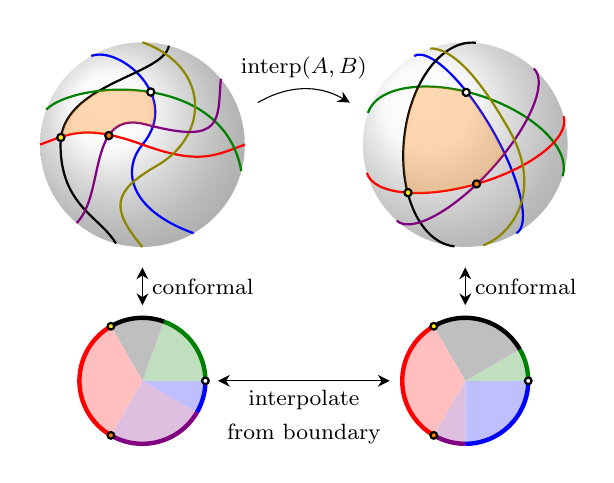
\begin{tikzpicture}

\begin{scope}[shift={(-4.3cm,-.2cm)},scale=1.3]

\shade[ball color=black!5, white, opacity=.5]
circle (1)
;

\path
(20:1.2) coordinate (X)
(270:1.2) coordinate (X1)
;

\draw[thick,blue]
(-60:1) .. controls +(160:.7) and +(50:-.3) ..
(0,0) .. controls +(50:.6) and +(20:.3) .. (120:1)
;

\draw[thick,red]
(0:1) .. controls +(200:.3) and +(-20:.6) ..
(0,0) .. controls +(-20:-.6) and +(20:.3) .. (0:-1)
;

\draw[thick]
(75:1) .. controls +(260:.3) and +(90:.6) ..
(0:-.8) .. controls +(90:-.6) and +(120:.3) .. (75:-1)
;

\draw[thick,green!50!black]
(-20:-1) .. controls +(45:.4) and +(100:1) .. (-15:1)
;

\draw[thick,olive]
(270:1) .. controls +(130:.5) and +(210:.5) ..
(-55:.25) .. controls +(210:-.6) and +(-20:.7) .. (90:1)
;

\draw[thick,violet]
(40:1) .. controls +(85:-.4) and +(-15:.8) ..
(80:.2) .. controls +(-15:-.6) and +(45:.4) .. (50:-1)
;

\begin{scope}

\clip
(50:-1) arc (230:40:1)
.. controls +(85:-.4) and +(-15:.8) ..
(80:.2) .. controls +(-15:-.6) and +(45:.4) .. (50:-1)
;

\clip
(75:1) .. controls +(260:.3) and +(90:.6) ..
(0:-.8) .. controls +(90:-.6) and +(120:.3) .. (75:-1)
arc (-105:75:1)
;

\clip
(-20:-1) .. controls +(45:.4) and +(100:1) .. (-15:1)
arc (-15:-200:1)
;

\clip
(-60:1) .. controls +(160:.7) and +(50:-.3) ..
(0,0) .. controls +(50:.6) and +(20:.3) .. (120:1)
arc (120:300:1)
;

\clip
(0:-1) arc (180:0:1)
.. controls +(200:.3) and +(-20:.6) ..
(0,0) .. controls +(-20:-.6) and +(20:.3) .. (0:-1)
;

\fill[orange,opacity=0.3]
(0,0) circle (1);

\end{scope}

\draw[thick,fill=white]
(81:.52) circle (1pt)
;

\draw[thick,fill=yellow]
(175:.8) circle (1pt)
;

\draw[thick,fill=orange]
(165:.34) circle (1pt)
;

\end{scope}

\begin{scope}[shift={(-.2cm,-.2cm)},scale=1.3, rotate=-60]

\shade[ball color=black!5, white, opacity=.5]
circle (1)
;

\begin{scope}[rotate=60]
\path
(160:1.2) coordinate (Y)
(270:1.2) coordinate (Y1)
;
\end{scope}

\begin{scope}[rotate = 0]
\draw[thick,blue]
(1,0) arc (0:180:1 and .3)
;\end{scope}

\begin{scope}[rotate = 42]
\draw[thick,green!50!black]
(1,0) arc (0:180:1 and .5)
;\end{scope}

\begin{scope}[rotate = 144]
\draw[thick]
(1,0) arc (0:180:1 and .6)
;\end{scope}

\begin{scope}[rotate = 256]
\draw[thick,red]
(1,0) arc (0:180:1 and .4)
;\end{scope}

\begin{scope}[rotate = 288]
\draw[thick,violet]
(1,0) arc (0:180:1 and .35)
;\end{scope}

\begin{scope}
\clip
(1,0) arc (0:180:1 and .3) arc (180:360:1);
\begin{scope}[rotate = 42]
\clip
(1,0) arc (0:180:1 and .5) arc (180:360:1);
\begin{scope}[rotate = 102]
\clip
(1,0) arc (0:180:1 and .6) arc (180:360:1);
\begin{scope}[rotate = 144]
\clip
(1,0) arc (0:180:1 and .35) arc (180:360:1);
\begin{scope}[rotate = -32]

\clip
(1,0) arc (0:180:1 and .4) arc (180:360:1);

\fill[orange,opacity=0.3]
(0,0) circle (1);

\end{scope}
\end{scope}
\end{scope}
\end{scope}
\end{scope}

\draw[thick,olive]
(170:1) .. controls +(60:.3) and +(0:-.3) ..
(80:.45) .. controls +(0:.7) and +(80:.3) .. (-20:1)
;

\draw[thick,fill=white]
(149:.51) circle (1pt)
;

\draw[thick,fill=yellow]
(280:.73) circle (1pt)
;

\draw[thick,fill=orange]
(166:-.4) circle (1pt)
;

\end{scope}

\begin{scope}[shift={(-4.3cm,-3.2cm)},scale=.8]

\fill[green!50!black!25] (0,0) -- (0:1) arc (0:70:1);
\fill[black!25] (0,0) -- (70:1) arc (70:120:1);
\fill[red!25] (0,0) -- (120:1) arc (120:240:1);
\fill[violet!25] (0,0) -- (240:1) arc (240:330:1);
\fill[blue!25] (0,0) -- (330:1) arc (330:360:1);

\draw[ultra thick,green!50!black] (0:1) arc (0:70:1);
\draw[ultra thick] (70:1) arc (70:120:1);
\draw[ultra thick,red] (120:1) arc (120:240:1);
\draw[ultra thick,violet] (240:1) arc (240:330:1);
\draw[ultra thick,blue] (330:1) arc (330:360:1);

\draw[thick,fill=white]
(0:1) circle (1.5pt)
;

\draw[thick,fill=yellow]
(120:1) circle (1.5pt)
;

\draw[thick,fill=orange]
(240:1) circle (1.5pt)
;

\path
(90:1.2) coordinate (X2)
(0:1.2) coordinate (X3)
;

\end{scope}

\begin{scope}[shift={(-.2cm,-3.2cm)},scale=.8]

\fill[green!50!black!25] (0,0) -- (0:1) arc (0:30:1);
\fill[black!25] (0,0) -- (30:1) arc (30:120:1);
\fill[red!25] (0,0) -- (120:1) arc (120:240:1);
\fill[violet!25] (0,0) -- (240:1) arc (240:270:1);
\fill[blue!25] (0,0) -- (270:1) arc (270:360:1);

\draw[ultra thick,green!50!black] (0:1) arc (0:30:1);
\draw[ultra thick] (30:1) arc (30:120:1);
\draw[ultra thick,red] (120:1) arc (120:240:1);
\draw[ultra thick,violet] (240:1) arc (240:270:1);
\draw[ultra thick,blue] (270:1) arc (270:360:1);

\draw[thick,fill=white]
(0:1) circle (1.5pt)
;

\draw[thick,fill=yellow]
(120:1) circle (1.5pt)
;

\draw[thick,fill=orange]
(240:1) circle (1.5pt)
;

\path
(90:1.2) coordinate (Y2)
(180:1.2) coordinate (Y3)
;

\end{scope}

\path[->]
(X) edge[bend left] node[auto] {\footnotesize $\text{interp}(A,B)$} (Y)
;

\path[<->]
(X1) edge node[auto] {\footnotesize conformal} (X2)
(Y1) edge node[auto] {\footnotesize conformal} (Y2)
(Y3) edge node[auto,align=center] {\footnotesize interpolate \\ \footnotesize from boundary} (X3)
;

\end{tikzpicture}
\end{center}

\caption{$\interp(A,B)$ defined on a $2$-cell.}
\label{figure-interp}

\end{figure}

For each $\sigma \in \mc{V}_{2}$, fix a choice of $3$ distinct elements $\upsilon_1,\upsilon_2,\upsilon_3 \in \mc{V}_{0}$ with $\upsilon_i <_\vv \sigma$; lets say the $3$ lexicographically smallest elements. These are the sign sequences of $3$ vertices of the boundary of $\cell(A,\sigma)$ for $A \in \real(\mc{M})$.
Let $p_i = (\cos (2\pi i/3), \sin (2\pi i/3)) \in \sphere^1$ for $i \in \{1,2,3\}$ be the $3$ points spaced uniformly about the unit circle with $p_3 = e_1$.
Let
\[ \conf_{A,\sigma}: \Ball^2 \to \cell(A,\sigma) \]
be the unique homeomorphism as in Theorem \ref{theorem-conformal} that is conformal on the interior and respectively sends $p_i$ to the vertex with sign sequence $\upsilon_i$, so $\cell(A,\upsilon_i) = \{\conf_{A,\sigma}(p_i)\}$.

For the 0-cells there is only one possibility, since a 0-cell is just a single point, so~for $\upsilon \in \mc{V}_{0}$,
let $\interp(A,B;\cell(B,\upsilon)) = \cell(A,\upsilon)$.

For each $\tau \in \mc{V}_{1}$, fix a sign sequence $\sigma \in \mc{V}_{2}$ such that $\sigma >_\vv \tau$ and let\vspace*{-3pt}
\[\phi_{A,\tau} : [0,1]_\mb{R} \to \partial{}\Ball^2\] be the positively oriented constant speed parameterization of the arc\vspace*{-3pt}
\[
\conf_{A,\sigma}^{\,-1}(\cell(A,\tau)).
\]
Let\vspace*{-5pt}
\[ \interp(A,B) = \conf_{A,\sigma}^{\phantom1} \circ \phi_{A,\tau}^{\phantom1} \circ \phi_{B,\tau}^{-1} \circ \conf_{B,\sigma}^{-1} \quad
\text{on } \cell(B,\tau).\]

For each $\sigma \in \mc{V}_{2}$, define
$ \phi_{A,B,\sigma} : \Ball^2 \to \Ball^2 $ by\vspace*{-3pt}
\[ \phi_{A,B,\sigma}(x) = \|x\| \left(\conf_{A,\sigma}^{-1} \circ \interp(A,B)^{\phantom1} \circ \conf_{B,\sigma}^{\phantom1}(x/\|x\|) \right) \]
for $x \neq 0$, let $\phi_{A,B,\sigma}(0)=0$,
and let\vspace*{-3pt}
\[ \interp(A,B) = \conf_{A,\sigma}^{\phantom1} \circ \phi_{A,B,\sigma}^{\phantom1} \circ \conf_{B,\sigma}^{-1} \quad
\text{on } \cell(B,\sigma).\]

\begin{lemma}\label{lemma-interp}
For every rank $3$ oriented matroid $\mc{M}$, $\interp$ is continuous on \hbox{$\real(\mc{M}) \times \real(\mc{M})$} and $A* \interp(A,B) = B$.
\end{lemma}

\begin{observation}\label{observation-interp-id}
The restriction of $\interp$ to the diagonal is the identity, \ie $\interp(A,A) = \id \in \hom(\sphere^2)$.
\end{observation}

\begin{observation}\label{observation-orthinterp}
Since $A*Q_1Q_1^{-1} \interp(A,B) Q_2 = B*Q_2 $,\vspace*{-3pt}
\[ \interp(A*Q_1,B*Q_2) = Q_1^{-1} \circ \interp(A,B) \circ Q_2. \]
\end{observation}

\begin{lemma}\label{lemma-path}
Let $S_k$ be a sequence of oriented simple closed curves in $\sphere^2$ that converge to an oriented simple closed curve $S_\infty$ in Fréchet distance, and let $a_k,b_k \in S_k$ such that $a_k \to a_\infty$ and $b_k \to b_\infty$. Then, the oriented paths $P_k \subset S_k$ from $a_k$ to $b_k$ converge to the oriented path $P_\infty \subset S_\infty$ from $a_\infty$ to $b_\infty$ in Fréchet distance.
\end{lemma}

\begin{proof}
For $x,y \in \sphere^1$, let $[x,y]_{\sphere^1}$ be the counter-clockwise arc from $x$ to $y$.
By~the hypotheses of the lemma, there is a sequence $\eps_k \to 0$ from above such that \hbox{$\|a_k - a_\infty\| < \eps_k$}, $\|b_k - b_\infty\| < \eps_k$,
and there a sequence of embeddings $f_k : \sphere^1 \to \sphere^2$ with $f_k(\sphere^1) = S_k$
such that for all $u \in \sphere^1$, $\|f_k(u) - f_\infty(u)\| < \eps_k $.
Additionally, we~choose $f_k$ so that the orientation on $S_k$ is the direction $f_k(u)$ traverses $S_k$ as~$u$ moves counter-clockwise around $\sphere^1$.
Let $P_k{}^\circ = P_k\setminus\{a_k,b_k\}$ denote the relative interior of the path $P_k$.
Fix $w \in \sphere^1$ such that ${f_\infty(w) \in P_\infty^{\,\circ}}$.
That is, $f_\infty(w)$ is on the interior of the arc of $S_k$ from $a_\infty$ to $b_\infty$.
By choosing $k$ sufficiently large, $\eps_{k}$ is sufficiently small, so that we may assume the following,
\[
\|f_\infty(w) -a_\infty\| > 2\eps_{k}, \quad
\|f_\infty(w) -b_\infty\| > 2\eps_{k}, \quad \text{and} \quad
\|b_\infty - a_\infty\| > 4\eps_k.
\]
Let $x_k \in \sphere^1$ be the first point clockwise of $w$ such that
$\|f_\infty(x_k) - a_\infty\| = 2\eps_k$
and $y_k \in \sphere^1$ be the first point counter-clockwise of $w$ such that
$\|f_\infty(y_k) - b_\infty\| = 2\eps_k$.
Starting from $f_\infty(w)$ and traversing $P_\infty$ we reach $f_\infty(y_k)$ before $b_\infty$, so
$f_\infty(y_k) \in P_\infty^{\,\circ}$.
For $u \in [w,y_k]_{\sphere^1}$, we have
\[ \|f_k(u) - b_\infty\| \geq \| f_\infty(u) - b_\infty \| - \|f_k(u) -f_\infty(u)\| > 2\eps_k -\eps_k = \eps_k, \]
but $\|b_k - b_\infty\| < \eps_k$, so while traversing $S_k$ from $f_k(w)$ to $f_k(y_k)$ we never get close enough to $b_\infty$ to reach $b_k$,
and analogously for $f_k(x_k)$ and $a_k$,
so the points $f_k(x_k),f_k(w),f_k(y_k)$ appear on $P_k{}^\circ$ in that order.

Let $\tilde x_k, \tilde y_k \in \sphere^1$ where $f_k (\tilde x_k) = a_k$ and $f_k (\tilde y_k) = b_k$, and
let
\[ A_k = [\tilde x_\infty,x_k]_{\sphere^1} \cup [\tilde x_k,x_k]_{\sphere^1} \quad \text{and}\quad
B_k = [y_k, \tilde y_\infty]_{\sphere^1} \cup [y_k, \tilde y_k]_{\sphere^1}
\]
\[ \alpha_k = \sup \{ \|f_\infty(u)-a_\infty\| :u \in A_k \} \quad \text{ and} \quad
\beta_k = \sup \{ \|f_\infty(u)-b_\infty\| :u \in B_k \}.
\]
Since $x_k,\tilde x_k \to \tilde x_\infty$ and $y_k, \tilde y_k \to \tilde y_\infty$, we have $\alpha_k,\beta_k \to 0$. Observe that
\begin{align*}
\sup \{ \|f_k(u)-f_\infty(v)\| &:u \in [\tilde x_k,x_k]_{\sphere^1},v \in [\tilde x_\infty,x_k]_{\sphere^1} \} \\
& \leq \sup \{ \|f_k(u) -a_\infty \| : u \in A_k \} + \sup \{ \|f_\infty(v) -a_\infty \| : v \in A_k \} \\
& < \eps_k +2\alpha_k,
\end{align*}
and similarly
$\sup \{ \|f_k(u)-f_\infty(v)\| :u \in [y_k,\tilde y_k]_{\sphere^1},v \in [y_k,\tilde y_\infty]_{\sphere^1} \} < \eps_k +2\beta_k $.

For $k\geq 3$,
let $u_k : [\nicefrac{1}{k},1-\nicefrac{1}{k}]_\mb{R} \to \sphere^1$ be a counter-clockwise parameterization of the arc from $x_k$ to $y_k$, and define $g_k,h_k : [0,1]_\mb{R} \to \sphere^2$ as follows.
For $t \in [\nicefrac{1}{k},1-\nicefrac{1}{k}]_\mb{R}$, let
\[ g_k(t) = f_k \circ u_k(t) \quad \text{and} \quad h_k(t) = f_\infty \circ u_k(t),\]
and on the rest of $[0,1]_\mb{R}$ complete $g_k$ and $h_k$ to respective parameterizations of $P_k$ and $P_\infty$.
We now have
\[\begin{array}{r@{\ <\ }l@{\quad \text{for}\quad }r@{\ \in\ }l}
\|g_k(t)-h_k(t)\| & \eps_k +2\alpha_k & t & [0,\nicefrac{1}{k}]_\mb{R}, \\
\|g_k(t)-h_k(t)\| & \eps_k & t & [\nicefrac{1}{k},1-\nicefrac{1}{k}]_\mb{R}, \\
\|g_k(t)-h_k(t)\| & \eps_k +2\beta_k & t & [1-\nicefrac{1}{k},1]_\mb{R},
\end{array}\]
and $\alpha_k,\beta_k,\eps_k \to 0$. Therefore, $P_k \to P_\infty$ in Fréchet distance.
\end{proof}

\begin{proof}[Proof of Lemma \ref{lemma-interp}]
First, we show that $A* \interp(A,B) = B$, by showing that $\interp(A,B)$ is defined by building up a map that sends each cell of $B$ to the corresponding cell of $A$.
In the case $\upsilon \in \mc{V}_0$, this is immediate from the definition.
In the case $\tau \in \mc{V}_1$, $\phi_{B,\tau}^{-1}$ is defined so that $\hbox{$\phi_{B,\tau}^{-1} \circ \conf_{B,\sigma}^{-1}(\cell(B,\tau))$} = [0,1]_\mb{R}$, and this is bijective, which also means $\conf_{A,\sigma}^{\phantom1} \circ \phi_{A,\tau}^{\phantom1}([0,1]_\mb{R}) = \cell(A,\tau)$.
In the case $\sigma \in \mc{V}_2$, $\interp(A,B)$ is a composition of bijections sending $\cell(B,\sigma)$ to the unit ball, which is then sent to itself, and then to $\cell(A,\sigma)$.

Next, we show $\interp(A,B) \in \hom(\sphere^2)$.
By definition $\conf_{A,\sigma}$ and $\conf_{A,\sigma}^{-1}$ and $\phi_{A,\tau}$ are continuous.
And, $\phi_{A,B,\sigma}$ is a composition of continuous functions except at the origin, where $\phi_{A,B,\sigma}$ is also continuous, since $\|\phi_{A,B,\sigma}(x)\| = \|x\|$.
We just have to check that the definition of $\interp(A,B)$ on each 1-cell agrees with the definition of $\interp(A,B)$ on the $2$-cells with that 1-cell on the boundary.
Let $\sigma \in \mc{V}_2$, $\tau \in \cov(\mc{M})$ such that $\tau <_\vv \sigma$, and let $x_k \in \cell(B,\sigma)$ such that $x_k \to x \in \cell(B,\tau)$. Then,
\begin{align*}
\interp(A,B;x_k)
& \to \conf_{A,\sigma}^{\phantom1} \circ \phi_{A,B,\sigma}^{\phantom1} \circ \conf_{B,\sigma}^{-1}(x) \\
&\hspace*{2.8mm} = \conf_{A,\sigma}^{\phantom1} \circ \conf_{A,\sigma}^{-1} \circ \interp(A,B)^{\phantom1} \circ \conf_{B,\sigma}^{\phantom1} \circ \conf_{B,\sigma}^{-1}(x) \\
&\hspace*{2.8mm} = \interp(A,B;x),
\end{align*}
since $\| \conf_{B,\sigma}^{-1}(x) \| = 1$. Thus, $\interp(A,B) \in \hom(\sphere^2)$.

Finally, we show that $\interp(A,B)$ depends continuously on $A$ and $B$.
The vertices of $A$ depend continuously on $A$ by Lemma~\ref{lemma-vertex}, and likewise for $B$.
By Lemma~\ref{lemma-path}, this implies that each 1-cell of $A$ and $B$ varies continuously, and therefore the conformal maps defining $\interp(A,B)$ vary continuously by Theorem \ref{theorem-conformal}.
\end{proof}

\Subsection{Topology of pseudolinear realization spaces}

\begin{proof}[Proof of Theorem \ref{theorem-pseudoreal-contract}]
By the topological representation theorem, $\realo(\mc{M})$ is non-empty \cite{folkman1978oriented}.
For $A \in \mc{A} \in \realo(\mc{M})$, we define a strong deformation retraction $\rho$ from $\realo(\mc{M})$ to $\mc{A}$.
For each $\mc{B} \in \realo(\mc{M})$, fix $B \in \mc{B}$. Let
\begin{gather*}
\rho : \realo(\mc{M}) \times [0,1]_\mb{R} \to \realo(\mc{M}),\\\rho(\mc{B},t) = A*\ho(\interp(A,B),t)\orth_3.
\end{gather*}
Observe that $\rho(\mc{B},t)$ does not depend on the choice of $B \in \mc{B}$ by Observation \ref{observation-orthinterp} and since $\ho$ is $\orth_3$-equivariant with respect to precomposition (right action). Indeed, for any other choice $B' \in \mc{B}$, there is $Q \in \orth_3$ such that $B' = B*Q$, and we have
\begin{align*}
A*\ho(\interp(A,B'),t)\orth_3
&= A*\ho(\interp(A,B) \circ Q,t)\orth_3 \\
&= A*\ho(\interp(A,B),t)Q\orth_3 \\
&= \rho(\mc{B},t).
\end{align*}
Furthermore, $\rho$ is continuous by Lemma \ref{lemma-interp} and is a strong deformation retraction by Theorem \ref{theorem-kneser-equivariant}.

If $\interp(A,B) \in \hom^+(\sphere^2)$, then $\ho(\interp(A,B),t) \in \hom^+(\sphere^2)$ for all $t \in [0,1]_\mb{R}$,
so the same deformation also shows that $\pog(\chi)$ is contractible.
\end{proof}

\begin{remark}
Note that if $\ho$ were $\orth_3$-equivariant with respect to postcomposition (left action), then $\rho$ would not depend on a choice of $A \in \mc{A}$, but the dependence on~$A$ is not a problem for our purposes.
\end{remark}

\section{Deforming weighted pseudocircle arrangements}\label{section-deforming}

In this section we prove Theorem \ref{theorem-grassman-pseudograssman}.
We first define several intermediate spaces in Section \ref{subsubsec-spaces}, and then define deformation retractions between these space. We then combine these deformations to produce a deformation retraction from $\pstief_{3,n}$ to $\stief_{3,n}$.
In Section \ref{subsubsec-f}, we deform each pseudocircle one at a time to become piecewise geodesic. More precisely, each pseudocircle becomes geodesic in each cell of the subdivision of the sphere by the previously deformed pseudocircles. We then perform a second round of deformations in Section \ref{subsubsec-h} where we coarsen the cell decomposition where the pseudocircles are geodesic, so that they are geodesic in decompositions with successively larger cells, until they become great circles; see Figure \ref{figure-deformations}. We then combine these deformations in Section \ref{subsubsec-g-finite} in a way that recursively performs a deformation for every permutation of the pseudocircles. The case $n=\infty$ is dealt with separately in Section \ref{subsubsec-g-infinite}. Finally, once we have deformed a arrangement of pseudocircles into an arrangement of great circles, we perform a continuous orthonormalization process in Section \ref{subsubsec-orth} to deform weighted great circle arrangements to Parseval frames.

\begin{figure}[htb]

\begin{center}
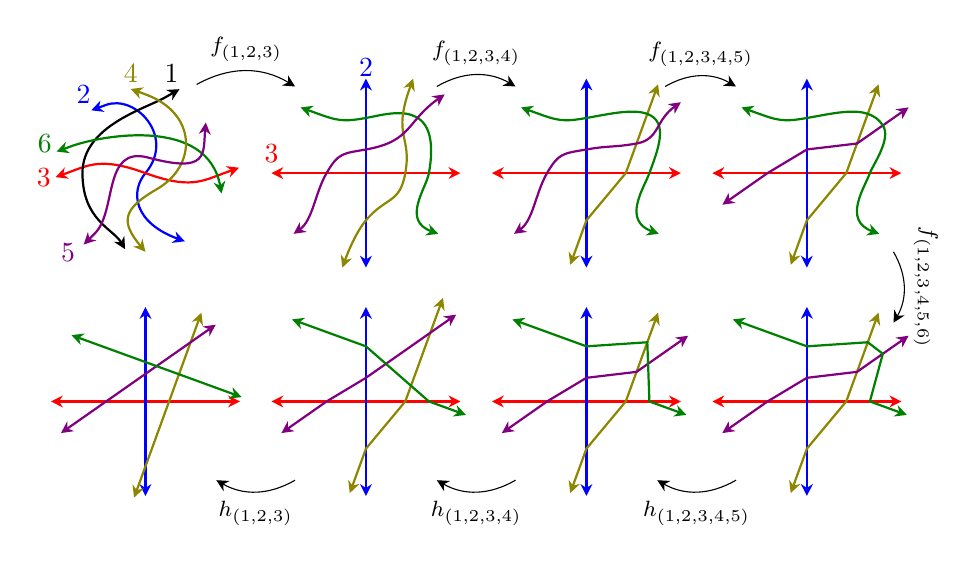
\begin{tikzpicture}[ampersand replacement=\&,scale=1]

\begin{scope}[shift={(-4.2cm,.5cm)},scale=1]

\path (60:1.3) coordinate (x1);

\draw[thick,blue,<->]
(-60:1) .. controls +(160:.7) and +(50:-.3) ..
(0,0) .. controls +(50:.6) and +(20:.4) .. (120:1) -- +(20:-.2)
node[shift={(-.1cm,.2cm)}] {2}
;

\draw[thick,red,<->]
(0:1) +(200:-.2) -- (0:1) .. controls +(200:.3) and +(-20:.6) ..
(0,0) .. controls +(-20:-.6) and +(20:.3) .. (0:-1) -- ++(20:-.15) node[shift={(-.15cm,0cm)}] {3}
;

\draw[thick,<->]
(75:1) +(210:-.2) node[shift={(-.1cm,.2cm)}] {1} -- (75:1) .. controls +(210:.3) and +(90:.6) ..
(0:-.8) .. controls +(90:-.6) and +(120:.3) .. (75:-1)
;

\draw[thick,green!50!black,<->]
(-20:-1) +(20:-.2) node[shift={(-.15cm,.1cm)}] {6} -- (-20:-1) .. controls +(20:.4) and +(100:1) .. (-15:1)
;

\draw[thick,olive,<->]
(270:1) .. controls +(130:.5) and +(210:.5) ..
(-55:.25) .. controls +(210:-.6) and +(-20:.7) .. (90:1) -- ++(-20:-.2) node[shift={(0cm,.2cm)}] {4}
;

\draw[thick,violet,<->]
(40:1) .. controls +(85:-.4) and +(-15:.8) ..
(80:.2) .. controls +(-15:-.6) and +(45:.4) .. (50:-1) -- ++(45:-.2) node[shift={(-.2cm,-.1cm)}] {5}
;

\end{scope}

\begin{scope}[shift={(-1.4cm,.5cm)}]

\path (-.9,1.1) coordinate (y1);
\path (.9,1.1) coordinate (x2);

\draw[thick,red,<->]
(-1.2,0) node[above] {3} -- (1.2,0)
;

\draw[thick,blue,<->]
(0,-1.2) -- (0,1.2) node[above,yshift=-.1cm] {2}
;

\draw[thick,green!50!black,<->]
(130:1) +(-20:-.2) -- (130:1)
.. controls +(-20:.3) and +(10:-.3) ..
(0,.7) .. controls +(10:.3) and +(-100:-1) ..
(.8,0) .. controls +(-100:.2) and +(-20:-.5) ..
(-40:1.2)
;

\draw[thick,olive,<->]
(-.3,-1.2) .. controls +(70:.2) and +(50:-.2) ..
(0,-.6) .. controls +(50:.4) and +(80:-.4) ..
(.5,0) .. controls +(80:.5) and +(70:-.8) ..
(.6,1.2)
;

\draw[thick,violet,<->]
(40:-1.2) .. controls +(35:.3) and +(60:-.3) ..
(-.5,0) .. controls +(60:.3) and +(10:-.3) ..
(0,.3) .. controls +(10:.6) and +(35:-.6) ..
(1,1)
;

\end{scope}

\path[->]
(x1) edge[bend left] node[auto] {\footnotesize $f_{(1,2,3)}$} (y1)
;

\begin{scope}[shift={(1.4cm,.5cm)}]

\path (-.9,1.1) coordinate (y2);
\path (1,1.1) coordinate (x3);

\draw[thick,red,<->]
(-1.2,0) -- (1.2,0)
;

\draw[thick,blue,<->]
(0,-1.2) -- (0,1.2)
;

\draw[thick,olive,<->]
(0,-.6) +(70:-.6) -- (0,-.6) -- (.5,0) -- ++(70:.4) coordinate (a) -- ++(70:.4) coordinate (b) -- ++(70:.4)
;

\draw[thick,green!50!black,<->]
(130:1) +(-20:-.2) -- (130:1)
.. controls +(-20:.3) and +(10:-.3) ..
(0,.7) .. controls +(10:.3) and +(-20:-.2) ..
(b) .. controls +(-20:.3) and +(-110:-.3) ..
(.8,0) .. controls +(-110:.2) and +(-20:-.5) ..
(-40:1.2)
;

\draw[thick,violet,<->]
(40:-1.2) .. controls +(35:.3) and +(60:-.3) ..
(-.5,0) .. controls +(60:.3) and +(10:-.3) ..
(0,.3) .. controls +(10:.3) and +(10:-.3) ..
(a) .. controls +(10:.3) and +(35:-.4) ..
(1.2,.9)
;

\end{scope}

\path[->]
(x2) edge[bend left] node[auto] {\footnotesize $f_{(1,2,3,4)}$} (y2)
;

\begin{scope}[shift={(4.2cm,.5cm)}]

\path (-.9,1.1) coordinate (y3);
\path (1.1,-1) coordinate (x4);

\draw[thick,red,<->]
(-1.2,0) -- (1.2,0)
;

\draw[thick,blue,<->]
(0,-1.2) -- (0,1.2)
;

\draw[thick,olive,<->]
(0,-.6) +(70:-.6) -- (0,-.6) -- (.5,0) -- ++(70:.4) coordinate (a) -- ++(70:.4) coordinate (b) -- ++(70:.4)
;

\draw[thick,violet,<->]
(-.5,0) +(35:-.7) -- (-.5,0) -- (0,.3) -- (a) -- ++(35:.4) coordinate (c) -- ++(35:.4)
;

\draw[thick,green!50!black,<->]
(130:1) +(-20:-.2) -- (130:1)
.. controls +(-20:.3) and +(10:-.3) ..
(0,.7) .. controls +(10:.3) and +(-20:-.2) ..
(b) .. controls +(-20:.1) and +(-55:-.1) ..
(c) .. controls +(-55:.2) and +(-110:-.1) ..
(.8,0) .. controls +(-110:.2) and +(-20:-.5) ..
(-40:1.2)
;

\end{scope}

\path[->]
(x3) edge[bend left] node[auto] {\footnotesize $f_{(1,2,3,4,5)}$} (y3)
;

\begin{scope}[shift={(4.2cm,-2.4cm)}]

\path (1.1,1) coordinate (y4);
\path (-.9,-1) coordinate (x5);

\draw[thick,red,<->]
(-1.2,0) -- (1.2,0)
;

\draw[thick,blue,<->]
(0,-1.2) -- (0,1.2)
;

\draw[thick,olive,<->]
(0,-.6) +(70:-.6) -- (0,-.6) -- (.5,0) -- ++(70:.4) coordinate (a) -- ++(70:.4) coordinate (b) -- ++(70:.4)
;

\draw[thick,violet,<->]
(-.5,0) +(35:-.7) -- (-.5,0) -- (0,.3) -- (a) -- ++(35:.4) coordinate (c) -- ++(35:.4)
;

\draw[thick,green!50!black,<->]
(0,.7) +(-20:-1) -- (0,.7) -- (b) -- (c) -- (.8,0) -- ++(-20:.5)
;

\end{scope}

\path[->]
(x4) edge[bend left] node[midway,above,rotate=-90] {\footnotesize $f_{(1,2,3,4,5,6)}$} (y4)
;

\begin{scope}[shift={(1.4cm,-2.4cm)}]

\path (.9,-1) coordinate (y5);
\path (-.9,-1) coordinate (x6);

\draw[thick,red,<->]
(-1.2,0) -- (1.2,0)
;

\draw[thick,blue,<->]
(0,-1.2) -- (0,1.2)
;

\draw[thick,olive,<->]
(0,-.6) +(70:-.6) -- (0,-.6) -- (.5,0) -- ++(70:.4) coordinate (a) -- ++(70:.4) coordinate (b) -- ++(70:.4)
;

\draw[thick,violet,<->]
(-.5,0) +(35:-.7) -- (-.5,0) -- (0,.3) -- (a) -- ++(35:.4) coordinate (c) -- ++(35:.4)
;

\draw[thick,green!50!black,<->]
(0,.7) +(-20:-1) -- (0,.7) -- (b) -- (.8,0) -- ++(-20:.5)
;

\end{scope}

\path[->]
(x5) edge[bend left] node[auto] {\footnotesize $h_{(1,2,3,4,5)}$} (y5)
;

\begin{scope}[shift={(-1.4cm,-2.4cm)}]

\path (.9,-1) coordinate (y6);
\path (-.9,-1) coordinate (x7);

\draw[thick,red,<->]
(-1.2,0) -- (1.2,0)
;

\draw[thick,blue,<->]
(0,-1.2) -- (0,1.2)
;

\draw[thick,olive,<->]
(0,-.6) +(70:-.6) -- (0,-.6) -- (.5,0) -- ++(70:1.4)
;

\draw[thick,violet,<->]
(-.5,0) +(35:-.7) -- (-.5,0) -- (0,.3) -- ++(35:1.4)
;

\draw[thick,green!50!black,<->]
(0,.7) +(-20:-1) -- (0,.7) -- (.8,0) -- ++(-20:.5)
;

\end{scope}

\path[->]
(x6) edge[bend left] node[auto] {\footnotesize $h_{(1,2,3,4)}$} (y6)
;

\begin{scope}[shift={(-4.2cm,-2.4cm)}]

\path (.9,-1) coordinate (y7);

\draw[thick,red,<->]
(-1.2,0) -- (1.2,0)
;

\draw[thick,blue,<->]
(0,-1.2) -- (0,1.2)
;

\draw[thick,olive,<->]
(.3,0) +(70:-1.3) -- (.3,0) -- ++(70:1.2)
;

\draw[thick,violet,<->]
(-.5,0) +(35:-.7) -- ++(35:1.7)
;

\draw[thick,green!50!black,<->]
(0,.5) +(-20:-1) -- (0,.5) -- ++(-20:1.3)
;

\end{scope}

\path[->]
(x7) edge[bend left] node[auto] {\footnotesize $h_{(1,2,3)}$} (y7)
;

\end{tikzpicture}
\end{center}

\caption{An example of a pseudocircle arrangement being deformed to a great circle arrangement. The arrangements are projected to the plane so that geodesic arcs appear linear, with pseudocircle 1 sent to infinity except in the first arrangement at the top left.}
\label{figure-deformations}

\end{figure}

\subsection{Intermediate spaces}
\label{subsubsec-spaces}

For each non-repeating sequence $I = (i_1,\dots,i_m)$ with entries among $[n]_\mb{N}$ we will define spaces $X_I,Y_I,Z_I \subseteq \pstief_{3,n}$
and deformation retractions $f_I,g_I,h_I$ between these spaces. The inclusion relations between these spaces is summarized by the following diagram, with the deformations written above or next to the corresponding inclusion.
\begin{small}
\[\hspace*{-3mm}
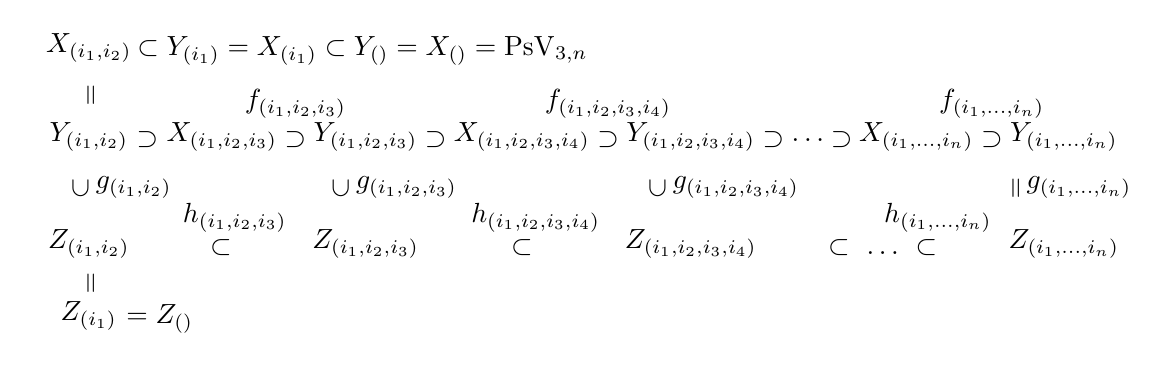
\begin{tikzpicture}
\matrix (m) [matrix of math nodes, row sep=2.2em,
column sep=.6em, text height=.5ex, text depth=0.25ex]
{
X_{(i_1,i_2)} \\
Y_{(i_1,i_2)} & X_{(i_1,i_2,i_3)} & Y_{(i_1,i_2,i_3)} & X_{(i_1,i_2,i_3,i_4)} & Y_{(i_1,i_2,i_3,i_4)} & \dots & X_{(i_1,\dots,i_n)} & Y_{(i_1,\dots,i_n)} \\[0.7em]
Z_{(i_1,i_2)} & & Z_{(i_1,i_2,i_3)} & & Z_{(i_1,i_2,i_3,i_4)} & & & Z_{(i_1,\dots,i_n)} \\[-0.6em]
Z_{(i_1)} \\
};
\path
(m-1-1) node[right,xshift=1.4em] {$ \subset Y_{(i_1)} = X_{(i_1)} \subset Y_{()} = X_{()} = \pstief_{3,n} $}
(m-1-1) to node[midway,sloped] {$=$} (m-2-1)
(m-2-7) to node[midway] {$\supset$} node[above,yshift=.4em] {$f_{(i_1,\dots,i_n)}$} (m-2-8)
(m-2-6) to node[midway] {$\supset$} (m-2-7)
(m-2-5) to node[midway] {$\supset$} (m-2-6)
(m-2-4) to node[midway] {$\supset$} node[above,yshift=.4em] {$f_{(i_1,i_2,i_3,i_4)}$} (m-2-5)
(m-2-3) to node[midway] {$\supset$} (m-2-4)
(m-2-2) to node[midway] {$\supset$} node[above,yshift=.4em] {$f_{(i_1,i_2,i_3)}$} (m-2-3)
(m-2-1) to node[midway] {$\supset$} (m-2-2)
(m-2-1) to node[midway,sloped,shift={(-.2em,-.3em)}] {$\supset$} node[right,shift={(-.1em,.2em)}] {$g_{(i_1,i_2)}$} (m-3-1)
(m-2-3) to node[midway,sloped,shift={(-.2em,-.9em)}] {$\supset$} node[right,shift={(-.7em,.2em)}] {$g_{(i_1,i_2,i_3)}$} (m-3-3)
(m-2-5) to node[midway,sloped,shift={(-.2em,-1.2em)}] {$\supset$} node[right,shift={(-1em,.2em)}] {$g_{(i_1,i_2,i_3,i_4)}$} (m-3-5)
(m-2-8) to node[midway,sloped,shift={(-.2em,-1.8em)}] {$=$} node[right,shift={(-1.7em,.2em)}] {$g_{(i_1,\dots,i_n)}$} (m-3-8)
(m-3-1) to node[midway] {$\subset$} node[above,shift={(.5em,.2em)}] {$h_{(i_1,i_2,i_3)}$} (m-3-3)
(m-3-3) to node[midway] {$\subset$} node[above,shift={(.5em,.2em)}] {$h_{(i_1,i_2,i_3,i_4)}$} (m-3-5)
(m-3-5) to node[midway] {$\subset\ \dots\ \subset$} node[above,shift={(2em,.2em)}] {$h_{(i_1,\dots,i_n)}$} (m-3-8)
(m-3-1) to node[midway,sloped] {$=$} (m-4-1)
node[right,xshift=1em] {$ = Z_{()} $}
;
\end{tikzpicture}
\]
\end{small}%
We define the spaces $X_I,Y_I,Z_I$
by giving conditions for a weighted pseudosphere arrangement $A = (\alpha_1,\dots,\alpha_n)$ to be in the space.
For this, let $S_i = (\aim \alpha_i)^{-1}(0)$ be the kernel of $\alpha_i$.
Recall $i \in I$ indicates that $i$ appears in the sequence $I$, and that $\proj_I(A)$ is the arrangement where each $\alpha_j$ for $j \not\in I$ is replaced with 0.
For $m = |I| \in \{0,1,2,3\}$, let $X_I$ be the set of arrangements $A$ such that $I$ is an independent set of $\cov(A)$. That is,

\vbox{
\begin{itemize}
\item
$X_{()} = \pstief_{3,n}$;
\item
$X_{(i_1)} \subset X_{()}$ where $\|\alpha_{i_1}\| \neq 0$;
\item
$X_{(i_1,i_2)} \subset X_{(i_1)}$ where $\|\alpha_{i_2}\| \neq 0$ and $S_{i_1} \neq S_{i_2}$;
\item
$X_{(i_1,i_2,i_3)} \subset X_{(i_1,i_2)}$ where $\|\alpha_{i_3}\| \neq 0$ and $S_{i_1} \cap S_{i_2} \cap S_{i_3} = \emptyset$.
\end{itemize}
}
For $m >3$, let $X_I = X_{(i_1,\dots,i_m)} \subset Y_{(i_1,\dots,i_{m-1})}$ such that $\|\alpha_{i_m}\| \neq 0$.
Informally, we use $X_{I}$ to first pick a basis and then subsequently pick non-zero weighted pseudocircles as long as one is available.

For $m \in \{0,1,2\}$, let $Y_I = X_I$.
For $m=3$, let $Y_{(i_1,i_2,i_3)} \subset X_{(i_1,i_2,i_3)}$ where $S_{i_1},S_{i_2},S_{i_3}$ are great circles.
Note that $S_i$ is a great circle if and only if $\alpha_i \in \Rpol{3}$.
For $m >3$, let $Y_I \subset X_I$ such that $S_{i_m}$ is antipodally symmetric and is geodesic in each of the $2$-cells of the subdivision of $\sphere^2$ by $S_{i_1},\dots,S_{i_{m-1}}$. That is, the pseudocircles indicated by the sequence $I$ are symmetric and piecewise geodesic with corners only on the pseudocircles appearing earlier in the sequence.

For $m \in \{0,1,2\}$, let $Z_I$ be the set of spanning weighted great circle arrangements, \ie vector configurations spanning $\Rpol{3}$.
For $m\geq 3$, let $Z_I \subseteq Y_I$ consist of arrangements $A$ such that every pseudocircle is antipodally symmetric, and for all $j \not\in I$, if~$\|\alpha_j\| \neq 0$ then $S_{j}$ is geodesic on each $2$-cell of $\proj_I(A)$. That is, all pseudocircles are piecewise geodesic with corners only on the pseudocircles appearing in the sequence, and those that appear in the sequence have corners only on those earlier in the sequence, and $-A = A * (-\id)$.

We will define strong equivariant deformation retractions $f_I$ from $X_I$ to $Y_I$ and $h_{I} = h_{(i_1,\dots,i_m)}$ from $Z_{(i_1,\dots,i_{m})}$ to $Z_{(i_1,\dots,i_{m-1})}$.
We then combine these to get strong deformation retractions $g_I$ from $Y_I$ to $Z_I$.
The deformations $f_I$ and $h_I$ for each $I$ ultimately fit together in equation \ref{equation-g} on page \pageref{equation-g} (or equation \ref{equation-g-infty} on page \pageref{equation-g-infty} for $n = \infty$) to give a deformation $g_{()}$ from $Y_{()} = \pstief_{3,n}$ to the space $Z_{()}$ of vector configurations that span $\Rpol{3}$.
To complete the deformation of Theorem~\ref{theorem-grassman-pseudograssman}, we~then perform a strong equivariant deformation retraction from great circles to Parseval frames by a continuous orthonormalization process.

Before defining the deformations we start with some properties of these spaces that will be needed.

\begin{lemma}\label{lemma-pseudocircle-dist}
Let $\alpha_1,\alpha_2$ be non-trivial weighted pseudocircles.
Then,
\[\left|\left(\|\alpha_1\|-\|\alpha_2\|\right)\right| \leq \dist(\alpha_1,\alpha_2) \leq \|\alpha_1\|+\|\alpha_2\|,\]
the lower bound is attained if and only if $\aim(\alpha_2) = \aim(\alpha_1)$,
and the upper bound is attained if and only if $\aim(\alpha_2) = \aim(\alpha_1)\circ(-\id)$.
\end{lemma}

\begin{proof}
The upper and lower bounds follow immediately from the definition of $\dist$.
Let $\theta_i = \aim(\alpha_i)$ and $S_i = \theta_i^{-1}(0)$,
and consider parameterizations of the sphere $\phi_i$ such that $\theta_i \circ \phi_i = \aim(e_3)$ as in the definition of $\dist$.

Suppose $\theta_2=\theta_1$. Then, we can use the same parameterization $\phi = \phi_1 = \phi_2$ for both pseudocircles.
For every $x$, we have
$\|(\|\alpha_1\|\phi(x) - \|\alpha_2\|\phi(x))\| = \left|(\|\alpha_1\|-\|\alpha_2\|)\right|$,
so $\dist(\alpha_1,\alpha_2) = \left|(\|\alpha_1\|-\|\alpha_2\|)\right|$.

Suppose $\theta_2\neq \theta_1$. Then, there is some point $p \in S_2 \setminus S_1$. For all parameterizations $\phi_i$ such that $\theta_i \circ \phi_i = \aim(e_3)$, we have $\phi_1(x) \neq p$ where $x = \phi_2^{-1}(p)$. Therefore, $\|\alpha_1\|\phi_1(x)$ and $\|\alpha_2\|\phi_2(x)$ are not parallel, so
$\|(\|\alpha_1\|\phi_1(x) - \|\alpha_2\|\phi_2(x))\| > \left|(\|\alpha_1\|-\|\alpha_2\|)\right|$,
so $\dist(\alpha_1,\alpha_2) > \left|(\|\alpha_1\|-\|\alpha_2\|)\right|$.

Suppose $\theta_2 = \theta_1\circ(-\id)$.
Then, for every pair of parameterization $\phi_i$, $\phi_1$ sends the upper hemisphere to the positive side of $S_1$, which is the reflection through the origin of the positive side of $S_2$, which is also the image by $\phi_2$ of the upper hemisphere.
Also, the maps $\phi_i$ preserve orientation, and reflection through the origin reverses orientation.
Therefore, the map $\phi_2^{-1}\circ (-\phi_1)$ is an orientation reversing homeomorphism of the sphere that sends the upper hemisphere to itself, so the restriction to the equator is an orientation reversing homeomorphism of a circle, and as such, must have a fixed point $x = \phi_2^{-1}\circ(-\phi_1)(x)$ on the equator. Therefore,
\[
\|(\|\alpha_1\|\phi_1(x) - \|\alpha_2\|\phi_2(x))\| = \|(\|\alpha_1\|\phi_1(x) + \|\alpha_2\|\phi_1(x))\| = \|\alpha_1\| + \|\alpha_2\|.
\]
Since every such pair of parameterizations $\phi_i$ must pass through an antipodal pair of points such as $\phi_1(x)$ and $\phi_2(x) = -\phi_1(x)$, we have $\dist(\alpha_1,\alpha_2) = \|\alpha_1\|+\|\alpha_2\|$.

Suppose $\theta_2 \neq \theta_1\circ(-\id)$.
Since a simple closed curve cannot be a proper subset of another simple closed curve, both $S_1 \setminus (-S_2)$ and $S_2 \setminus (-S_1)$ must be non-empty.
Furthermore, by compactness of the curves $S_i$, $S_1$ contains a closed arc $T_1$ that is bounded away from $-S_2$, and $S_2$ contains a closed arc $T_2$ that is bounded away from~$-S_1$. Let $X_1$ and $X_2$ be two semicircles that together form the equator. Let $\phi_1$ be a parameterization that sends $X_1$ to $T_1$, which means that $\phi_1$ must send $X_2$ to the closure of $S_1\setminus T_1$. Let $\phi_2$ be a parameterization that sends $X_2$ to $T_2$, which means that $\phi_2$ must send $X_1$ to the closure of $S_2\setminus T_2$.
Then,
For $x$ on the equator, either $\phi_1(x)$ is in $T_1$ or $\phi_2(x)$ is in $T_2$, so
no point on the equator is mapped by $\phi_1$ and $\phi_2$ to an antipodal pair of points,
which means that $\phi_2(x)$ is bounded away from $-\phi_1(x)$.
Therefore, $\|(\|\alpha_1\|\phi_1(x) - \|\alpha_2\|\phi_2(x))\|$ is bounded away from $\|\alpha_1\| + \|\alpha_2\|$ for all $x$ on the equator. Thus, $\dist(\alpha_1,\alpha_2) < \|\alpha_1\|+\|\alpha_2\|$.
\end{proof}

\begin{lemma}\label{lemma-reflections}
If $(\theta_1,\theta_2)$ is a pseudocircle arrangement and $\theta_2 = \theta_1 \circ (-\id)$,
then $\theta_2 = -\theta_1$. For kernels $(S_1,S_2)$, if $S_2 = -S_1$, then $S_2 = S_1$ and this pseudocircle is antipodally symmetric.
\end{lemma}

\begin{proof}
Let $S_i = \theta^{-1}(0)$ be the kernel of $\theta_i$ and suppose that $S_1$ and $S_2$ do not coincide.
Let $\pi$ be a closed path that traverses once around $S_2$ so that the positive side is on the left.
Then, $\pi$ crosses $S_1$ exactly twice; once at a point $p$ going from the negative side of $S_1$ to the positive side, and then again at a point $q$ going back from the positive side of $S_1$ to the negative side.
Since $\theta_2 = \theta_1 \circ (-\id)$, the reflection of $\pi$ through the origin is a path $-\pi$ that traverses $S_1$ so that the positive side is on the right.
Therefore, at the point $p$, $-\pi$ crosses $S_2$ from the negative side to the positive side, which implies that $\pi$ crosses $S_1$ at $-p$ from the negative side to the positive side.
We now have that $\pi$ crosses $S_1$ from the negative side to the positive side at both~$p$ and $-p$, and similarly $\pi$ crosses $S_1$ from the positive side to the negative side at both $q$ and $-q$, which means $\pi$ crosses $S_1$ at least 4 times, but that contradicts that $\pi$ must cross $S_1$ exactly twice.
Therefore, $S_1$ and $S_2$ must coincide, and hence must be antipodally symmetric.
To complete the second part of the lemma, observe that $S_2 = -S_1$ if and only if $\{\theta_2,-\theta_2\} \ni \theta_1 \circ (-\id)$.
\end{proof}

\begin{claim}\label{claim-sphericonvex}
For $m = |I| \geq 3$ and $A \in Y_I$, the $2$-cells of $\proj_I({A})$ are spherical convex polygons such that each edge is a 1-cell of $\proj_I({A})$.
\end{claim}

\begin{proof}
We proceed by induction. For $m=3$, each cell is an orthant of the sphere, which is a spherical triangle with 1-cell edges. Since $Y_I \subset Y_{(i_1,\dots,i_{m-1})}$, the $2$-cells of $\proj_{(i_1,\dots,i_{m-1})}(A)$ are spherical convex polygons with edges that are 1-cells by inductive assumption. At each $2$-cell $C$ such that $S_{i_m}$ intersects the interior of $C$, $S_{i_m}$ must intersect $C$ in a path $P$, since the restriction of $\proj_I({A})$ is homeomorphic to a 1-dimensional pseudosphere arrangement and $P = C \cap S_{i_m}$ is a 1-cell of that arrangement.
From the definition of $Y_I$, $P$ must be a geodesic arc through $C$, thereby subdividing $C$ into a pair of spherical convex polygons with edges that are 1-cells.
\end{proof}

\begin{claim}\label{claim-open-X}
For $m > 0$, $X_I$ is an open proper subset of $Y_{(i_1,\dots,i_{m-1})}$ in the induced metric topology on $Y_{(i_1,\dots,i_{m-1})}$.
\end{claim}

Note that $X_I$ is not generally open in the topology on $\pstief_{3,n}$.

\begin{proof}
Consider some $A \in Y_{(i_1,\dots,i_{m-1})}$, a generic configuration in $(\Rpol{3})^n \subset Y_{(i_1,\dots,i_{m-1})}$ will suffice. Then, $\proj_{[n]_\mb{N}\setminus i_m}(A) \in Y_{(i_1,\dots,i_{m-1})} \setminus X_I$, so $X_I$ is a proper subset of $Y_{(i_1,\dots,i_{m-1})}$.

To show $X_I$ is open, for each $A \in X_I$, we find a radius $r>0$ sufficiently small that every $B \in Y_{(i_1,\dots,i_{m-1})}$ within distance $r$ of $A$ is in $X_I$.
For $m =1$ or $m>3$, $r = \|\alpha_{i_m}\|$ suffices.
For $m \in \{2,3\}$, we may use
\[ r = \min \bigl\{\|\alpha_i\|:i\in I \bigr\} \cdot \inf\bigl\{ (\nicefrac{1}{2}) \|x -y\|:x \in P,\ y \in (S_{i_1} \cup \dots \cup S_{i_m}) \bigr\}, \]
where $P$ consists of a point in the interior of each $2$-cell of the subdivision of the sphere by $S_{i_1},\dots,S_{i_m}$.
For every $B \in Y_{(i_1,\dots,i_{m-1})}$ within distance $r$ from $A$, we have that the points of $P$ are each in the corresponding $2$-cell of $B$, which means $B \in X_I$.
\end{proof}

\subsection{The deformation $f_I$ from $X_I$ to $Y_I$}
\label{subsubsec-f}

For $m \in \{0,1,2\}$, let $f_I(A,t) = A$ be the trivial deformation.
We will split into cases where $m=3$ or $m >3$.
In both cases we assume that $\coord((i_1,i_2,i_3);A)$ is the identity, otherwise let
\[
f_I(A,t) = f_I(A*Q,t)*Q^{-1},
\]
where $Q = \coord((i_1,i_2,i_3);A)$.
Also, in both cases the deformation is defined by deforming the arrangement $B = (\beta_1,\dots,\beta_n) = \proj_I(A)$ to an arrangement $C$, which will be defined separately in each case. Recall that $\proj_I$ replaces all weighted pseudocircles with index not appearing in $I$ with the trivial pseudocircle, so $\beta_i = \alpha_i$ for $i \in I$ and $\beta_j = 0$ for $j \not\in I$.
Recall also that $i^+ = \sign(e_i)$ is the sign sequence with $(+)$ in the $i$-th place and $0$ elsewhere.

\subsubsection*{The case $m=3$.}
Let $C = (\gamma_1,\dots,\gamma_n)$ be defined by the following conditions. We~will show that these conditions determine a unique arrangement in Claim \ref{claim-well-defined-f3}.
For $i \not\in I$, $\gamma_i = 0$,
$\gamma_{i_3} = \|\alpha_{i_3}\|e_3$,
and for $k \in \{1,2\}$,
let
$\gamma_{i_k} \in \Rpol{3}$ be the unique vector such that
\begin{itemize}
\item
$\|\gamma_{i_k}\| = \|\alpha_{i_k}\|$,
\item
$\|\gamma_{i_k} -\gamma_{i_3}\| = \dist(\alpha_{i_k},\alpha_{i_3})$,
\item
$\langle \gamma_{i_2}, e_1 \rangle = 0$,
\item
$\langle \gamma_{i_2}, e_2 \rangle > 0$,
\item
$\gamma_{i_1}$ is perpendicular to $p_2 = \cell(B,{i_2}^+)$,
\item
and $\ot(C;i_1,i_2,i_3) = (+)$.
\end{itemize}
Let
\[ f_{I}(A,t) = A*\ho(\interp(B,C),1-t).\]

\begin{claim}\label{claim-well-defined-f3}
$f_I$ is well-defined for $m=3$.
\end{claim}

\begin{proof}
Since $A \in X_I$, $I$ is a basis of $A$, so $(\alpha_{i_1},\alpha_{i_2},\alpha_{i_3})$ is a spanning arrangement. Therefore, $S_{i_k} \neq S_{i_3}$ for $k \in \{1,2\}$, which implies by Lemma \ref{lemma-reflections} that $S_{i_k} \neq -S_{i_3}$, so by Lemma \ref{lemma-pseudocircle-dist},
\[ |(\|\alpha_{i_k}\| - \|\alpha_{i_3}\|)| < \dist(\alpha_{i_k},\alpha_{i_3}) < \|\alpha_{i_k}\| +\|\alpha_{i_3}\|. \]
The farthest point from $\gamma_{i_3}$ on the sphere of radius $\|\alpha_{i_k}\|$ centered at the origin is distance $\|\alpha_{i_k}\| +\|\alpha_{i_3}\|$ away, and the nearest point is distance $|(\|\alpha_{i_k}\| - \|\alpha_{i_3}\|)|$ away. Since $\dist(\alpha_{i_k},\alpha_{i_3})$ is strictly between these extremes, the spheres of radius $\|\alpha_{i_k}\|$ about the origin and radius $\dist(\alpha_{i_k},\alpha_{i_3})$ about $\gamma_{i_3}$ intersect in a circle $X_k$, which is parallel to $e_3^\bot$.
The circle $X_2$ contains exactly 2 points on $e_1^\bot$, and only one of these has positive 2nd coordinate.
Thus, $\gamma_{i_2}$ is well-defined.
Since we are assuming that $\coord((i_1,i_2,i_3);A)$ is the identity,
$p_2$ is on $e_3^\bot$, so the plane orthogonal to $p_2$ intersects the circle $X_1$ in exactly two points, and for only one of these two points does setting $\gamma_{i_1}$ to that point make $\ot(C;i_1,i_2,i_3)$ positive.
Thus, $\gamma_{i_1}$ is well-defined, so $C$ is well-defined, and therefore $f_I$ is well-defined.
\end{proof}

\begin{claim}\label{claim-deform-f3}
$f_I$ is a strong equivariant deformation retraction from $X_I$ to $Y_I$ for $m=3$.
\end{claim}

\begin{proof}
The weights and the order type of an arrangement $A$ remain unchanged as $A$ is deformed by $f_I$, so $f_I(A,t) \in X_I$ throughout the deformation.
Since $\gamma_{i_1},\gamma_{i_2},\gamma_{i_3} \in \Rpol{3}$, the kernel of $i_k$-th pseudocircle is a great circle, so $f_I(A,1) \in Y_I$. By Theorem~\ref{theorem-kneser-equivariant} and Lemma~\ref{lemma-interp}, $\ho$ and $\interp$ are continuous, so $f_I$ is continuous.
Recall that $f_I(A,t) = f_I(A*Q_0,t)*Q_0^{-1}$ where $Q_0 = \coord(I;A)$ by definition.
For $Q_1 \in \orth_3$,
we have ${\coord(I;A*Q_1) = Q_1^{-1}Q_0}$ by Lemma \ref{lemma-basis}, so
\begin{align*}
f_I(A*Q_1,t) & = f_I(A*Q_1Q_1^{-1}Q_0,t)*(Q_1^{-1}Q_0)^{-1} \\
& = f_I(A*Q_0,t)*Q_0^{-1}Q_1 \\
& = f_I(A,t)*Q_1,
\end{align*}
so $f_I$ is equivariant.
It only remains to show that $f_I$ is trivial on $Y_I$.

Let us consider $A\!\in\!Y_I$ such that $\coord(I;A)$ is the identity,
and for $k\!\in\!\{1,2,3\}$, let $p_k\!=\!\cell(A;{i_k}^+)$ as in the definition of $\coord$.
Then, $\alpha_{i_k}\!\in\!\Rpol{3}$. Since \hbox{$\coord(I;A)\!=\!\id$}, from the definition of $\coord$ we have that $p_1 = e_1$ and $p_2$ is on $e_3^\bot$, so $\alpha_{i_3}$ is parallel to $e_3$ and $\alpha_{i_2}$ is on $e_1^\bot$.
Since $\langle \alpha_{i_2},p_2 \rangle > 0$ and $p_2$ is on the half-plane in $e_3^\bot$ with positive 2nd coordinate, $\alpha_{i_2}$ is on the half-plane in $e_1^\bot$ with positive 2nd coordinate.
Since $\langle \alpha_{i_1},e_1 \rangle = \langle \alpha_{i_1},p_1 \rangle > 0$,
the vector $\alpha_{i_1} \times \alpha_{i_2}$ has positive 3rd coordinate.
Since $\ot(A;I) = (+)$,
$\langle \alpha_{i_1} \times \alpha_{i_2}, \alpha_{i_3} \rangle = \det(\alpha_{i_1},\alpha_{i_2},\alpha_{i_3})$ is positive, and since $\alpha_{i_3}$ is parallel to $e_3$, we have $\alpha_{i_3} = \|\alpha_{i_3}\|e_3 = \gamma_{i_3}$.
By Claim~\ref{claim-well-defined-f3}, $\gamma_{i_1}$ and $\gamma_{i_2}$ are uniquely determined by the conditions defining $C$, which are satisfied by $\alpha_{i_1}$ and $\alpha_{i_2}$, so \hbox{$\gamma_{i_k} = \alpha_{i_k}$} for $k\in\{1,2,3\}$. Therefore, $C=B$, so by Observation \ref{observation-interp-id} $\interp(B,C) = \id$, and since $\ho$ is a strong deformation retraction, $f_I(A,t) = A$. Thus, the restriction of $f_I$ to $Y_I$ is the trivial deformation, so $f_I$ is a strong deformation retraction.
\end{proof}

\subsubsection*{The case $m>3$.}
Let $C\!=\!(\gamma_1,\dots,\gamma_n)$ be defined as follows.
For $k\!<\!m$ let $\gamma_{i_k}\!=\!\beta_{i_k}$.
Let $\gamma_{i_m}$ be a copy of $\beta_{i_m}$ in the upper hemisphere that is straightened in each cell keeping the end points fixed, and a reflected copy in the lower hemisphere.
That is, we let
\[ H = \bigl\{(x_1,x_2,x_3) \in \sphere^2 :x_1 > 0 \text{ or } (x_1=0 \text{ and } x_2 \geq 0)\bigr\}, \]
\[ V = \bigcup_{k=1}^{m-1} S_{i_k}. \]
For $v \in V$, let
\[ \aim (\gamma_{i_m}; v) = \begin{cases}
\phantom{-}\aim (\beta_{i_m}; v) & v \in H, \\
{-}\aim (\beta_{i_m}; -v) & v \not\in H.
\end{cases}\]
Let $\gamma_{i_m}$ be defined on $\sphere^2 \setminus V$ such that $S_{i_m}$ is geodesic on all $2$-cells of $\proj_{(i_1,\dots,i_{m-1})} A$.
Let
\[ f_{I}(A,t) = A*\ho(\interp(B,C),1-t).\]

\begin{claim}\label{claim-deform-f}
$f_I$ is a well-defined strong equivariant deformation retraction from~$X_I$ to $Y_I$ for $m>3$.
\end{claim}

\begin{proof}
The $2$-cells of $\proj_{(i_1,\dots,i_{m-1})}(A)$ are spherical convex polygons by Claim \ref{claim-sphericonvex}, so the geodesic arc between any pair of points of a $2$-cell is entire\-ly in that cell, so $C$ is well-defined and $\cov(B)=\cov(C)$, so $f_I$ is well-defined.
Also, $f_I$ is continuous and equivariant by the same calculation as in the proof of Claim \ref{claim-deform-f3} above.
Since $C \in Y_I$ by definition, $f_I$ is an equivariant deformation from $X_I$ to $Y_I$.
Since the initial sequence of weighted pseudocircles $\alpha_{i_1},\dots,\alpha_{i_{m-1}}$ remain fixed throughout the deformation, we have for all $A \in X_I$ and $t \in [0,1]_\mb{R}$ that $f_I(A,t) \in Y_{(i_1,\dots,i_{m-1})}$, and since the norm of $\alpha_{i_m}$ also remains fixed, we have $f_I(A,t) \in X_I$, which implies that~$f_I$ is a deformation retraction.
If $A \in Y_I$ to start, then $f_I(A,t) = A$ is trivial, since $\beta_{i_m} = \gamma_{i_m}$, which implies $B=C$, so $f_I$ is a strong deformation retraction.
\end{proof}

Our goal is to eventually combine the deformations $f_I$ to deform the pseudocircles of an arrangement to be piecewise geodesic. For a given arrangement $A$, we could find a sequence $i_1,\dots,i_m$ such that $f_{(i_1,\dots,i_m)}\cdot f_{(i_1,\dots,i_{m-1})}\cdots f_{(i_1,i_2,i_3)}$ deforms the pseudocircles of $A$ to be piecewise geodesic, but this might not work for all sequence.
What we need is a single deformation that works for all arrangements in $\pstief_{3,n}$. We~will define such a deformation in Section \ref{subsubsec-g-finite} by recursively combining deformations to use all permutations of $[n]_\mb{N}$. One challenge that arises with this approach is that there could be one sequence $I$ that we can use to deform $A$ to be piecewise geodesic, but we first deform $A$ using another sequence $J$ that does not work. We would like to ensure that after deforming $A$ using the sequence $J$, we will still be able to use the sequence $I$. We will use the following claim to deal with this challenge.

\begin{claim}\label{claim-stable-f}
For all $p \in \{0,\dots,m{-}1\}$ and all $j \in [n]_\mb{N} \setminus \{i_1,\dots,i_p\}$,
if $A \in X_I \cap X_{(i_1,\dots,i_{p},j)}$ then $f_I(A,1) \in X_{(i_1,\dots,i_{p},j)}$.
\end{claim}

\begin{proof}
For $p=0$, the claim holds since $f_I$ preserves norm. In particular, for \hbox{$A \in X_{(j)}$}, the norm of the $j$-th pseudocircle never vanishes throughout the deformation $f_I(A,t)$.
Similarly for $p\geq 3$, the claim holds since
\[
f_I(A,t) \in X_I \subset Y_{(i_1,\dots,i_{m-1})} \subseteq Y_{(i_1,\dots,i_p)},
\]
so $f_I(A,1) \in Y_{(i_1,\dots,i_p)}$, and $f_I$ preserves norm.

For $p=1$ (or $p=2$), the claim holds since $f_I$ preserves order type. In particular, if $(i_1,j)$ (or $(i_1,i_2,j)$) is an ordered independent set of $\cov(A)$, then it remains independent throughout the deformation.
\end{proof}

\subsection{The deformation $h_{(i_1,\dots,i_m)}$ from $Z_{(i_1,\dots,i_m)}$ to $Z_{(i_1,\dots,i_{m-1})}$.}
\label{subsubsec-h}

We now define a deformation retraction $h_I = h_{(i_1,\dots,i_m)}$ from $Z_I = Z_{(i_1,\dots,i_m)}$ to $Z_{(i_1,\dots,i_{m-1})}$. If $m < 3$, this is the trivial deformation, so assume $m \geq 3$.

Recall from the definition of $Z_I$ that for $A \in Z_I$, $S_{i_1},S_{i_2},S_{i_3}$ are great circles, which means $\alpha_{i_1}, \alpha_{i_2},\alpha_{i_3} \in \Rpol{3}$.
We project from $\sphere^2$ to the real projective plane $\projplane$ (defined as a compactification of $\mb{R}^2$) by the 2-fold covering map $\proj_{\projplane}(\alpha_{i_1},\alpha_{i_2},\alpha_{i_3}) : \sphere^2 \to \projplane$ that sends $S_{i_1}$ to the horizon, and $S_{i_2}$ and $S_{i_3}$ to the horizontal and vertical axes respectively.
This map is given on $x \in \sphere^2 \setminus S_{i_1}$ by
\[ \proj_{\projplane}(\alpha_{i_1},\alpha_{i_2},\alpha_{i_3}; x) = \Bigl( \frac{\langle \alpha_{i_2}, x \rangle}{\langle \alpha_{i_1}, x \rangle}, \frac{\langle \alpha_{i_3}, x \rangle}{\langle \alpha_{i_1}, x \rangle} \Bigr), \]
where $\langle \cdot,\cdot \rangle$ is the inner product on $\Rpol{3}$ corresponding to the standard inner product on $\mb{R}^3$,
and the map is defined for $x \in S_{i_1}$ by continuous extension.
We do this projection so that we can make use of the vector space structure of $\mb{R}^2 \subset \projplane$ when defining $h_I$.

Recall that a \df{pseudoline} in $\projplane$ is a simple closed curve in the real projective plane that cannot be deformed to a point.
Let $\curves$ denote the space of all pseudolines in $\projplane$.
We give $\curves$ the metric that is the pull-back by $\proj_{\projplane}(e_1,e_2,e_3)$ of Fréchet distance on pseudocircles in $\sphere^2$.
By \df{pseudoline arrangement} we mean a sequence of pseudolines such that each pair of pseudolines either coincide or intersect at a single point, or such a sequence where some entries are $\projplane$ instead of a pseudoline.
Equivalently, a pseudoline arrangement is the projection of the kernels of a symmetric pseudocircle arrangement to the projective plane \cite[\S 6.2]{bjorner1999oriented}.
We say $L$ is a \df{pseudoline extension} of a pseudoline arrangement $(L_{i_1},\dots,L_{i_m})$ when $(L_{i_1},\dots,L_{i_m},L)$ is a pseudoline arrangement, \ie either $L = L_{i_j}$ for some $j$, or $L$ is a pseudoline that intersects each~$L_{i_j}$ exactly once.
Note that, unlike pseudocircles, we do not distinguish orientation for pseudolines.

Since the pseudocircles of an arrangement in $Z_I$ are antipodally symmetric, these project to pseudolines in $\projplane$, which we denote $L_i = L_i(A) = \proj_{\projplane}(\alpha_{i_1},\alpha_{i_2},\alpha_{i_3};S_i)$.
We will define the deformation $h_I$ by deforming the pseudolines $L_i$ and lifting these to deformations of weighted pseudocircles.
An important feature of the deformations that we will use is that each pseudoline $L_j$ for $j \in \compl{I} = [n]_\mb{N} \setminus I$ deforms in a way that depends only on $L_{i_1},\dots,L_{i_m}$, and the initial position of $L_{j}$, but distinct pseudolines deform independently of each other.
Claim~\ref{claim-pseudoline-lift} below shows that this is a valid way to define such a deformation.

Let
\[
L_{(j_1,\dots,j_k)}(A) = (L_{j_1}(A),\dots,L_{j_k}(A))
\quad \text{and} \quad
\tilde Z_I = L_I(Z_I).
\]
We call a partial map
\[ \tilde \lambda : \tilde Z_I \times \curves \times [0,1]_\mb{R} \not\to \curves \]
an \df{extension deformation process} on $\tilde Z_I$ when, for all $\tilde A \in \tilde Z_I$, $\lambda_0 \in \curves$, and $t \in [0,1]_\mb{R}$, the following hold.
\begin{enumerate}
\item
$\tilde \lambda(\tilde A, \lambda_0, 0) = \lambda_0$.
\item
$\tilde \lambda(\tilde A, \lambda_0, t)$ is defined,
provided that $\lambda_0$ is a pseudoline extension of $\tilde A$ and $\lambda_0$ is linear in each cell of $\tilde A$.
\item
$\tilde \lambda$ is continuous on the domain where it is defined.
\end{enumerate}
We say $\eta: Z_I \times [0,1]_\mb{R} \to \pstief_{3,n}$ is a deformation of $Z_I$ \df{induced} by the extension deformation process $\tilde \lambda$ on $\tilde Z_I$ when, for all $A \in Z_I$, $t \in [0,1]_\mb{R}$, and $j \in \compl{I}$, the following hold.
\begin{enumerate}
\item
$\wei(\eta(A,t)) = \wei(A)$.
\item
$\proj_{I}(\eta(A,t)) = \proj_{I}(A)$.
\item
$\eta(A,t)$ is antipodally symmetric and $L_{j}(\eta(A,t)) = \tilde \lambda(L_I(A),L_j(A),t)$.
\end{enumerate}

\begin{claim}\label{claim-pseudoline-lift}
{If} $\tilde \lambda$ is an extension deformation process on $\tilde Z_I$ such that
\[ \bigl(\tilde \lambda(\tilde A, L_1, t),\dots,\tilde \lambda(\tilde A, L_{n}, t) \bigr) \]
is a pseudoline arrangement for every $\tilde A \in \tilde Z_I$, $t \in [0,1]_\mb{R}$, and every pseudoline arrangement $(L_1,\dots,L_n)$ where $(L_{i_1},\dots,L_{i_m}) = \tilde A$,
{then} there is a unique deformation~$\eta$ of $Z_I$ induced by $\tilde \lambda$, and $\eta$ is $\orth_3$-equivariant.
\end{claim}

\begin{proof}
We first show uniqueness by demonstrating that $\tilde \lambda$ does not need to keep track of the orientations of the pseudocircles, as these can be tracked throughout the deformation.
Note that this depends crucially on the fact that a weight of zero cannot become positive.
Otherwise, a trivial pseudocircle could become non-trivial, and the orientation of that pseudocircle could not be determined from its kernel. The issue here is that the $\mb{Z}_2$-action on the space $Z_I$ generated by reversing the orientation of a pseudocircle is not free. Specifically, reversing the orientation of a pseudocircle that has vanished does not actually change the arrangement. To deal with this, we partition into classes $W_A$ where this action is either free or trivial, so that we can keep track of orientations as an arrangement deforms, provided that it remains within a single class. Afterwords, we will have to show that the resulting deformation is continuous across classes.
Let
\[ W_A = \left\{B \in \pstief_{3,n}:-B = B*(-\id),\ \wei(B) = \wei(A),\ \proj_I(B) = \proj_I(A) \right\} \]
be the space of symmetric weighted pseudocircle arrangements where the weight of each pseudocircle is fixed to match that of $A$,
and the pseudocircles indexed by $I$ coincide with those of $A$.
Let ${J = \{j \in \compl{I}: \|\alpha_j\| \neq 0 \}}$ be the indices of the non-zero elements of $A$.
Let $\widetilde W_A = L_{(1,\dots,n)}(W_A)$
be the space of pseudoline arrangements extending $L_{i_1},\dots,L_{i_m}$ by $|J|$ pseudolines, keeping the original indices.
For $B = (\beta_1,\dots,\beta_n) \in W_A$, we have $\dist(\beta_j,- \beta_j) = 2\|\alpha_j\| >0$, so the $\mb{Z}_2$-action reversing the orientation of the $j$-th element is free on $W_A$, provided that $j \in J$.
Therefore, $W_A$ is a $2^{|J|}$-fold covering of $\widetilde W_A$.
Let $\tilde A = L_I(A)$ and
\[
\Lambda : (Z_I\cap W_A) \times [0,1]_\mb{R} \to \widetilde W_A, \quad
\Lambda(B,t) = \bigl( \tilde \lambda(\tilde A, L_1(B), t),\dots, \tilde \lambda(\tilde A, L_n(B),t) \bigr).
\]
By the hypotheses of the claim, $\Lambda(B,t)$ is a pseudoline arrangement, so there are~$2^{|J|}$ arrangements in $W_A$ that project to $\Lambda(B,t)$, one arrangement for each choice of orientation for each of the pseudolines indexed by $J$.
Since covering maps have the unique homotopy lifting property, the deformation $\Lambda$ lifts to a continuous deformation~$\eta_A$ of $Z_I \cap W_A$ in $W_A$, and $\eta_A$ is unique in this regard.

Let $\eta$ be the function $\eta(A,t) = \eta_A(A,t)$ for each $A \in Z_I$.
By definition, if there is a deformation $\eta'$ of $Z_I$ induced by $\lambda$, then $\eta'(A,t) \in W_A$ and each pseudocircle projects to a pseudoline that deforms according to $\tilde \lambda$, so $\eta' = \eta$ is the unique lift of $\Lambda$.
Hence~$\eta$ is the unique deformation induced by $\tilde \lambda$, provided that $\eta$ is continuous.

Next, we show that $\eta$ is continuous where it is defined.
Let $\eta_{A,i}$ be the deformation of the $i$-th weighted pseudocircle of $\eta_A$, so that
$\eta_A = {\eta_{A,1} \times \dots \times \eta_{A,n}}$.
Note that some of the weighted pseudocircles may vanish and reappear elsewhere as $A$ varies over the domain of $\eta$, but $L_{i_1},\dots,L_{i_m}$ cannot vanish by the definition of $Z_I$.
Consider $A_k \to A_\infty \in Z_I$ and $t_k \to t_\infty \in [0,1]_\mb{R}$. Let
\[ A_k = (\alpha_{k,1},\dots,\alpha_{k,n}) = ((r_{k,1},\theta_{k,1}),\dots,(r_{k,n},\theta_{k,n})), \]
and let $M_k$ be the linear transformation sending
\[
\alpha_{\infty,i_1},\alpha_{\infty,i_2},\alpha_{\infty,i_3}\quad\text{to}\quad \alpha_{k,i_1},\alpha_{k,i_2},\alpha_{k,i_3},
\]
and let $N_k \in \hom(\sphere^2)$ be $M_k$ followed by projecting radially to the sphere.
Recall that $\{\alpha_{k,i_1},\alpha_{k,i_2},\alpha_{k,i_3}\}$ is a basis for the vector space $\Rpol{3}$ by definition of $Z_I$, so $M_k$ is a well-defined invertible linear transformation and $M_k \to M_\infty=\id$ in the operator norm.

For each $i$ such that $r_{\infty,i} > 0$, for $k$ large enough, we have that $r_{k,i} > 0$, so we may let
\[ B_k = (\beta_{k,1},\dots,\beta_{k,n}) \in W_{A_\infty}, \]
where
\[ \beta_{k,i} = \begin{cases}
(r_{\infty,i},\theta_{k,i} \circ N_k) & r_{\infty,i} > 0, \\
0 & r_{\infty,i} = 0.
\end{cases}\]
Since $\theta_{k,i} \to \theta_{\infty,i}$ and $N_k \to \id$, we have $B_k \to A_\infty$, and since $\eta_{A_\infty}$ is a continuous deformation in $W_{A_\infty}$, we have $\eta(B_k,t_k) = \eta_{A_\infty}(B_k,t_k) \to \eta(A_\infty,t_\infty)$.

The distance between the $i$-th element $\alpha$ of $\eta(A_k,t_k)$ and $\beta$ of $\eta(B_k,t_k)$ is, by~definition of Fréchet distance, the infimum over maps
\[
\text{from}\quad\|\alpha_{k,i}\|S \subset \mb{R}^3\quad\text{to}\quad\|\beta_{k,i}\|T = \|\alpha_{\infty,i}\|T \subset \mb{R}^3
\]
respecting the orientations of $S$ and $T$, where $S$ and $T$ are the kernel of $\aim(\alpha)$ and $\aim(\beta)$.
Let $\|\cdot\|_\text{op}$ denote the operator norm of a linear transformation.
We can obtain $\|\alpha_{\infty,i}\|T$ from $\|\alpha_{k,i}\|S$ by first scaling by $\|\alpha_{\infty,i}\|/\|\alpha_{k,i}\|$, which moves each point at most $\left| \| \alpha_{\infty,i} \| - \| \alpha_{k,i} \| \right|$, then applying $M_k$, which moves each point at most $\| \alpha_{\infty,i} \| \cdot \|M_k -\id \|_{\textrm{op}}$, and then projecting radially to $\|\alpha_{\infty,i}\| \sphere^2$, which moves each point at most $\| \alpha_{\infty,i} \| \cdot | \|M_k \|_{\textrm{op}} -1 |$. Hence, we can bound the distance to $\beta$ from $\alpha$ as the sum of the distances for each of these three steps, which gives,
\begin{multline*}
\dist(\eta(B_k,t_k), \eta(A_k,t_k))\\
\leq \max_{i \in [n]_\mb{N}} \Bigl( \bigl| \| \alpha_{\infty,i} \| - \| \alpha_{k,i} \| \bigr| +\| \alpha_{\infty,i} \| \bigl( \|M_k -\id \|_{\textrm{op}} +\bigl| \|M_k \|_{\textrm{op}} -1 \bigr| \bigr) \Bigr).
\end{multline*}
Since $\|\alpha_{k,i}\| \to \|\alpha_{\infty,i}\|$ and $M_k \to \id$, we have $\dist(\eta(B_k,t_k), \eta(A_k,t_k)) \to 0$, so
$\eta(A_k,t_k) \to \eta(A_\infty,t_\infty)$, which means $\eta$ is continuous.
Thus, $\eta$ is the deformation of~$Z_I$ induced by $\tilde \lambda$.

Finally, we show that $\eta$ is $\orth_3$-equivariant. For $Q \in \orth_3$, we have
\begin{align*}
L_i(A*Q)
= \Bigl\{ \Bigl( \frac{\langle Q^*\alpha_{i_2}, x \rangle}{\langle Q^*\alpha_{i_1}, x \rangle}, \frac{\langle Q^*\alpha_{i_3}, x \rangle}{\langle Q^*\alpha_{i_1}, x \rangle} \Bigr) :x \in Q^* S_i \Bigr\}
= L_i(A).
\end{align*}
That is, applying an orthogonal transformation to a weighted pseudocircle arrangement in $A \in Z_I$, does not change its image in the projective plane, since the projection $\proj_{\projplane}(\alpha_{i_1},\alpha_{i_2},\alpha_{i_3})$ also changes by the same transformation.
Therefore,
\[
L_j(\eta(A,t)*Q) = L_j(\eta(A,t)),\quand \tilde \lambda(L_I(A*Q),L_j(A*Q),t) = \tilde \lambda(L_I(A),L_j(A),t),
\]
so $L_j(\eta(A*Q,t)) = L_j(\eta(A,t))$, which means $L_j(\eta(A*Q,t)) = L_j(\eta(A,t)*Q)$.
Also $\proj_I(\eta(A*Q,t)) = \proj_I(A*Q) = \proj_I(\eta(A,t)*Q)$,
so $\eta(A*Q,t) = \eta(A,t)*Q$, which means $\eta$ is $\orth_3$-equivariant.
\end{proof}

We will define $h_I$ as the deformation of $Z_I$ induced by an extension deformation process $\tilde \lambda$ as in Claim~\ref{claim-pseudoline-lift}.
We first choose some arbitrary $A \in Z_{I}$ and let $\tilde A = L_I(A) \in \tilde Z_{I}$, and choose an arbitrary pseudoline extension $\lambda(0)$ that is linear on the cells of $\tilde A$. To define $\tilde \lambda$, we define a deformation $\lambda(t)$ of the pseudoline $\lambda(0)$, and then let $\tilde \lambda(\tilde A,\lambda(0),t) = \lambda(t)$. Note that $\lambda(t)$ may depend on $\tilde A = (L_{i_1},\dots,L_{i_m})$ and $\lambda(0)$.

\subsubsection*{The case $m>3$.}
For $m >3$, $h_I$ is the deformation of $Z_I$ induced by the extension deformation process $\tilde \lambda$ where $\lambda(t) = \tilde \lambda(\tilde A, \lambda(0), t)$ is defined as follows.
Let $\lambda(t) = \lambda(0)$ be fixed unless $\lambda(0)$ intersects $L_{i_m}$ at a single point $p(0)$ that is in the interior of a $2$-cell $C$ of the subdivision of $\projplane$ by $L_{i_1},\dots,L_{i_{m-1}}$.
Note that $C$ might be unbounded as a subset of $\mb{R}^2 = \projplane\setminus L_{i_1}$.
Otherwise, let $\lambda$ be fixed on the complement of $C$, and let $\lambda$ evolve in $C$ as follows; see Figure \ref{figure-hI>3}.
Let $a,b$ be the points where $\lambda(0)$ meets the boundary of $C$, and
$p(1)$ be the point where the segment $[a,b]_{C}$ intersects $L_{i_m}$,
and
\begin{gather*}
p(t) = t p(1) + (1-t) p(0), \\
\lambda(t) \cap C = \left[a,p(t),b\right]_{C}.
\end{gather*}

\begin{figure}[htb]
\begin{center}
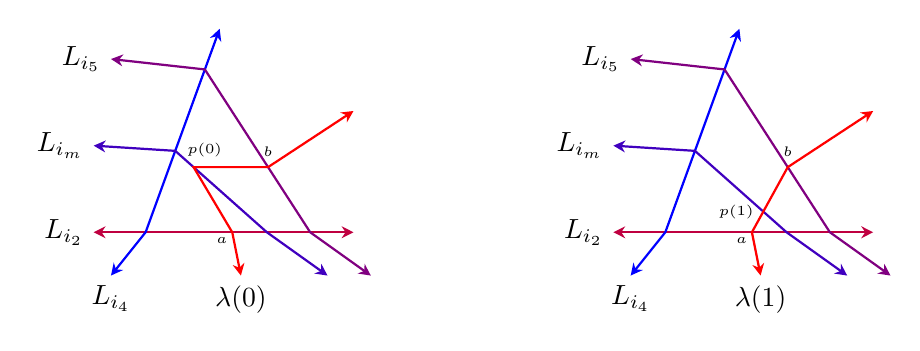
\begin{tikzpicture}[scale=1.1,every node/.style={black}]

\draw[thick,purple,<->]
(-1,0) node[left] {$L_{i_2}$} -- (2,0);

\draw[blue,thick,<->]
(-.8,-.5) node[below] {$L_{i_4}$} -- (-.4,0) -- ++(70:1) coordinate (a) -- ++(70:1) coordinate (b) -- ++(70:.5);

\draw[violet,thick,<->]
(-.8,2) node[left] {$L_{i_5}$} -- (b) -- (1.5,0) coordinate (c) -- (2.2,-.5);

\draw[blue!50!violet,thick,<->]
(-1,1) node[left] {$L_{i_m}$} -- (a) -- (1,0) coordinate (d) -- (1.7,-.5);

\draw[red,thick,<->]
(.7,-.5) node[below] {$\lambda(0)$} -- (.6,0) node[below left,shift={(2pt,2pt)}] {\tiny $a$} -- ($(a)!.2!(d)$) node[above,shift={(4pt,0pt)}] {\tiny $p(0)$} -- ($(b)!.6!(c)$) node[above] {\tiny $b$} -- (2,1.4);

\begin{scope}[shift={(6,0)}]

\draw[thick,purple,<->]
(-1,0) node[left] {$L_{i_2}$} -- (2,0);

\draw[blue,thick,<->]
(-.8,-.5) node[below] {$L_{i_4}$} -- (-.4,0) -- ++(70:1) coordinate (a) -- ++(70:1) coordinate (b) -- ++(70:.5);

\draw[violet,thick,<->]
(-.8,2) node[left] {$L_{i_5}$} -- (b) -- (1.5,0) coordinate (c) -- (2.2,-.5);

\draw[blue!50!violet,thick,<->]
(-1,1) node[left] {$L_{i_m}$} -- (a) -- (1,0) coordinate (d) -- (1.7,-.5);

\draw[red,thick,<->]
(.7,-.5) node[below] {$\lambda(1)$} -- (.6,0) node[below left,shift={(2pt,2pt)}] {\tiny $a$} coordinate (e) -- ($(b)!.6!(c)$) node[above] {\tiny $b$} coordinate (f) -- (2,1.4);

\node[left] at (intersection of a--d and e--f) {\tiny $p(1)$};

\end{scope}

\end{tikzpicture}
\caption{Points used to define $\lambda(t)$ for $m>3$.}
\label{figure-hI>3}
\end{center}
\end{figure}

\begin{claim}\label{claim-lambda-def}
For $m >3$, $\lambda(t)$ is well-defined and is a pseudoline extension of $L_{i_1},\dots,L_{i_m}$.
\end{claim}

\begin{proof}
We may assume that $\lambda(0)$ is a pseudoline extension of $(L_{i_1},\dots,L_{i_{m-1}})$ that passes through the interior of the cell $C$ where it intersects $L_{i_m}$, otherwise the deformation is trivial.
Since $\lambda(0)$ is a pseudoline extension, $\lambda(0)$ intersects $C$ in a single connected component, so $\lambda(0) \cap C$ is a polygonal path with a pair of well-defined endpoints $a,b$, and at most one of these points may be on the horizon $L_{i_1}$.
By Claim \ref{claim-sphericonvex} and $Z_I \subset Y_I$ we know that $S_{i_1},\dots,S_{i_{m-1}}$ subdivide $\sphere^2$ into spherical convex polygons, so $C$ is a convex polygonal region of $\mb{R}^2 = \projplane \setminus L_{i_1}$. Recall that $C$ might be unbounded.
From the definition of $Z_I$, we know that $L_{i_m} \cap C$ is a segment through~$C$ that subdivides $C$ into two convex polygonal regions.
From the definition of $C$, we~know that $\lambda(0)$ crosses $L_{i_m}$ at a single point $p(0) \in C$, which implies that $a,b$ are separated in $C$ by $L_{i_m}$, and therefore the segment $[a,b]_{C}$ intersects $L_{i_m}$ at a single point $p(1) \in C$.
Hence $p(t) \in (L_{i_m} \cap C)$ is well-defined, and $\lambda(t) \cap C$ is a well-defined polygonal path that intersects $L_{i_m}$ at a single point. Since $\lambda(t)$ is fixed outside of~$C$ and $\lambda(t)$ is a path in $C$ between fixed endpoints on the boundary of $C$, $\lambda(t)$ is a simple closed curve. Since $\lambda(t)$ is a deformation of the pseudoline $\lambda(0)$, $\lambda(t)$ is a pseudoline.
By~definition, $\lambda(0)$ starts as a pseudoline extension of $L_{i_1},\dots,L_{i_m}$, and~$\lambda(t)$ only deforms in the interior of the cell $C$ of $(L_{i_1},\dots,L_{i_{m-1}})$ where it meets $L_{i_m}$ at a~single point $p(t)$, so $\lambda(t)$ is a pseudoline extension of $(L_{i_1},\dots,L_{i_{m-1}})$ throughout the deformation.
\end{proof}

\begin{claim}\label{claim-lambda-continuous}
For $m >3$, $\tilde \lambda$ is continuous on the domain where it is defined. Hence, $\tilde \lambda$ is an extension deformation process on $\tilde Z_I$.
\end{claim}

\begin{proof}
Let $\tilde A_k = (L_{k,i_1},\dots,L_{k,i_m}) \in \tilde Z_{I}$, $\lambda_k(0) \in \curves$ be a pseudoline extension that is linear on cells of $\tilde A_k$, and $t_k \in [0,1]_\mb{R}$ such that $\tilde A_k \to \tilde A_\infty$, $\lambda_k(0) \to \lambda_\infty(0)$, and $t_k \to t_\infty$.
Note that $L_{k,i_1} = L_{i_1}$, $L_{k,i_2} = L_{i_2}$, and $L_{k,i_3} = L_{i_3}$ are fixed at the horizon, horizontal axis, and vertical axis respectively.
Let $\lambda_k(t) = \tilde \lambda(\tilde A_k,\lambda_k(0),t)$ be defined as above.
Our goal is to show that $\lambda_k(t_k) \to \lambda_\infty(t_\infty)$.

Since there are only finitely many rank $3$ oriented matroids on $n$ elements, we may assume that $\tilde A_k$ has the same covector set for all $k \in \mb{N}$, otherwise partition into finitely many subsequences by the covector sets of the $\tilde A_k$ and show convergence to $\lambda_\infty(t_\infty)$ for each subsequence separately.

If $\lambda_k(0) = L_{k,i_m}$, then $\lambda_k$ is fixed throughout the deformation, so the limit converges and we are done.
Otherwise, let $p_k(0) = \lambda_k(0) \cap L_{k,i_m}$.
If $p_{k}(t)$ is on one of the pseudolines $L_{k,i_1},\dots,L_{k,i_{m-1}}$, then $\lambda_k$ is fixed again and we are done.
Otherwise, let~$C_k$ be the $2$-cell of the subdivision of $\mb{R}^2$ by $L_{k,i_2},\dots,L_{k,i_{m-1}}$ that contains $p_{k}(t)$ in its interior.

By Lemma~\ref{lemma-vertex}, the vertices of $\tilde A_k$ converge to the corresponding vertices of $\tilde A_\infty$.
Consequently, by Lemma~\ref{lemma-path} the 1-cells of $\tilde A_k$ converge to corresponding 1-cells or vertices of $\tilde A_\infty$.
In particular, $p_k(0) \to p_\infty(0)$ and $\{a_k,b_k\} \to \{a_\infty,b_\infty\}$ where these are defined in the same way as $a,b$ above.
Since $L_{k,i_m} \cap C_k$ is a segment approaching $L_{\infty,i_m} \cap C_\infty$ and $\lambda_k(0) \cap C_k$ is a distinct segment approaching $L_{\infty,i_m} \cap C_\infty$, we have $p_k(1) \to p_\infty(1)$, since the intersection point of a pair of non-parallel segments depends continuously on their end points.
Since $\lambda_k(t)$ is defined continuously in terms of $\lambda_k(0)$, $a_k$, $b_k$, $p_k(0)$, and $p_k(1)$, we have $\lambda_k(t_k) \to \lambda_\infty(t_\infty)$.
Thus, $\tilde \lambda$ is continuous on the domain where it is defined, and therefore is an extension deformation process on~$\tilde Z_I$.
\end{proof}

Let $\Lambda(A,t) = \bigl(\tilde \lambda(\tilde A,L_1,t),\dots,\tilde \lambda(\tilde A,L_n,t)\bigr)$.

\begin{claim}\label{claim-lambda-arrangement}
For $m>3$, $\Lambda(A,t)$ is a pseudoline arrangement. Hence, $h_I$ is a well-defined $\orth_3$-equivariant deformation of $Z_I$.
\end{claim}

\newcommand{\xj}{{j'}}

\begin{proof}
Let $J = \{ j \in \compl{I}: \|\alpha_j\| > 0 \}$, and let $\lambda_j(t) = \tilde\lambda(\tilde A, L_j,t)$.
Since the pseudolines $\lambda_j(t)$ deform according to their initial positions, any initially identical pairs of pseudolines remain identical throughout the deformation. Consider $L_j,L_\xj$ distinct. We may assume that at least one of these is deforming, and it suffices to show that the number of crossings does not change in the cell where it deforms.
Assume $L_j$ crosses~$L_{i_m}$ at a point $p(0)$ in the interior of a $2$-cell $C$ of $L_{i_1},\dots,L_{i_{m-1}}$.

Suppose $L_j,L_\xj$ meet in the interior of the cell. Then, $L_j,L_\xj$ alternate around the boundary of $C$, and since points on the boundary of $C$ remain fixed, $\lambda_j(t),\lambda_\xj(t)$ meet in $C$ for all $t$. Since $\lambda_j(t),\lambda_\xj(t)$ are linear segments in the cells $C_1,C_2 \subset C$ divided by $L_{i_m}$, they can meet in at most one point in each cell $C_1,C_2$. If $\lambda_j(t),\lambda_\xj(t)$ met at a point in both $C_1$ and $C_2$, then they would alternate around the boundary of both cells, which would imply that they do not alternate around the boundary of $C$.
Thus, $\lambda_j(t),\lambda_\xj(t)$ meet at only a single point in $C$ for all $t$.

Now suppose $L_j,L_\xj$ do not meet in the interior of $C \in \mc{C}$.
Then, they do not alternate around the boundary of $C$, $C_1$, or $C_2$,
and we may assume $L_j,L_\xj$ both meet the segment $L_{i_m} \cap C$, otherwise they would never alternate around $C$, $C_1$, or $C_2$ as a result of the deformation.
Since $\lambda_j(t),\lambda_\xj(t)$ are fixed on the boundary of $C$, they still do not alternate around the boundary of $C$ at $t=1$, so $\lambda_j(1),\lambda_\xj(1)$ do not meet in $C$, which implies that they also do not alternate around the boundary of $C_1$ or $C_2$.
Therefore, the order of the points $p_j(t),p_{\xj}(t)$ where $\lambda_j(t),\lambda_\xj(t)$ meet the segment $L_{i_m} \cap C$ is the same for $t=0$ as for $t=1$.
That is, $p_{j}(1)-p_{\xj}(1)= r (p_{j}(0)-p_{\xj}(0))$ for some $r >0$, so
$p_{j}(t)-p_{\xj}(t)= (tr +(1-t)) (p_{j}(0)-p_{\xj}(0))$, which implies $\lambda_j(t),\lambda_\xj(t)$ do not alternate around the boundary of $C_1$ or $C_2$ for all $t$. Hence, $\lambda_j(t),\lambda_\xj(t)$ never meet in $C$ throughout the deformation.

Thus, each pair of pseudolines $\lambda_j(t),\lambda_\xj(t)$ either coincide or cross exactly once throughout the deformation, so $\Lambda(A,t)$ is a pseudoline arrangement, and therefore by Claims \ref{claim-lambda-continuous} and \ref{claim-pseudoline-lift}, $h_I$ is well-defined as the equivariant deformation induced by~$\tilde\lambda$.
\end{proof}

\begin{claim}\label{claim-deform-h}
For $m >3$, $h_I = h_{(i_1,\dots,i_m)}$ is a strong $\orth_3$-equivariant deformation retraction from $Z_{(i_1,\dots,i_m)}$ to $Z_{(i_1,\dots,i_{m-1})}$.
\end{claim}

\begin{proof}
We have already that $h_I$ is an $\orth_3$-equivariant deformation of $Z_I$ by Claim \ref{claim-lambda-arrangement}.
Since $\lambda(t)$ is linear in each cell of $\tilde A = (L_{i_1},\dots,L_{i_{m}})$, we have $h_I(A,t) \in Z_I$,
and since $\lambda(1)$ is linear in each cell of $(L_{i_1},\dots,L_{i_{m-1}})$, we have $h_I(A,1) \in Z_{(i_1,\dots,i_{m-1})}$,
so $h_I$ is a deformation retraction from $Z_I$ to $Z_{(i_1,\dots,i_{m-1})}$.
For $A \in Z_{(i_1,\dots,i_{m-1})}$ and $\lambda(0) = L_j$, we have that $\lambda(0)$ is linear in each cell of $(L_{i_1},\dots,L_{i_{m-1}})$, so $p(1) = p(0)$, which implies $\lambda(t) = \lambda(0)$ is a trivial deformation, and therefore $h_I(A,t) = h_I(A,0)$ is trivial. Thus, $h_I$ is a strong deformation retraction.
\end{proof}

\subsubsection*{The case $m=3$.}
For $m=3$, let $h_I$ be the deformation of $Z_I$ induced by the extension deformation process $\tilde \lambda$ defined by $\lambda(t) = \tilde \lambda(\tilde A, \lambda(0), t)$
for a pseudoline extension $\lambda(0)$ of $\{\tilde A\} = \{(L_{i_1},L_{i_2},L_{i_3})\} = \tilde Z_{I}$ as follows.

If $\lambda(0)$ is a straight line,
then let $\lambda$ be fixed.
Equivalently, $\lambda$ is fixed unless $\lambda(0)$ intersects $L_{i_1}$, $L_{i_2}$, $L_{i_3}$ at three distinct points that are not collinear.
Assume this is~so, and let $p_k(0) = \lambda(0) \cap L_{i_k}$ for $k \in \{1,2,3\}$.

We define $\lambda(t)$ as a polygonal path with moving points $p_k(t)$ as vertices.
For points $a,b \in \projplane$, let $[a,b]_\oplus$ denote the segment between $a,b$ contained in a single quadrant of $\projplane$ when such a segment exists and is unique, and let
\[
[a,b,c,\dots]_\oplus = [a,b]_\oplus \cup [b,c]_\oplus \cup \cdots.
\]
With this we have $\lambda(0) = [p_1(0),p_2(0),p_3(0),p_1(0)]_{\oplus}$.

Let $p_1 = p_1(t) = p_1(0)$ be fixed throughout the deformation.
Let $P$ be the line through the origin $0$ that is perpendicular to the line though $\{0,p_1\}$.
Let $q_0$ be the point where the line $P$ meets $\lambda(0)$; see Figure \ref{figure-q0}.

We define $\lambda(t)$ as the polygonal path consisting of a segment in one quadrant that pivots around the point $q_0$ and then extends beyond the axis as rays in the fixed direction of $p_1$.
We pivot at such a rate that the exterior angle at the vertices of $\lambda(t)$ is $(\nicefrac{\pi}{2})(1-t)$ once this becomes smaller than the initial exterior angle at $t=0$; see Figure \ref{figure-hI3}.
Specifically, let $\lambda(1)$ be the line though $\{q_0,p_1\}$, let \hbox{$\phi(0) \in (-\nicefrac{\pi}{2},\nicefrac{\pi}{2})_\mb{R}$} be the signed angle from $\lambda(1)$ to the line though $\{p_2(0),p_3(0)\}$ and $\phi(t) = \min(\phi(0),(\nicefrac{\pi}{2})(1-t))$, let $Q(t)$ be the line though $q_0$ at angle $\phi(t)$ from~$\lambda(1)$, and let $p_2(t) = Q(t) \cap L_{i_2}$ and $p_3(t) = Q(t) \cap L_{i_3}$.
Finally, let
\[ \lambda(t) = [p_1,p_2(t),p_3(t),p_1]_{\oplus}. \]

\begin{figure}[htb]
\begin{center}

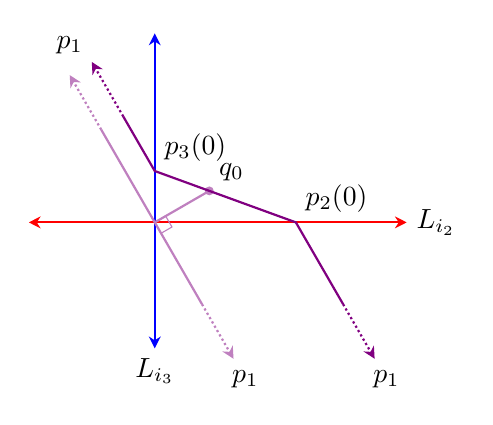
\begin{tikzpicture}[scale=.8]

\draw[thick,red,<->]
(-2,0) -- (4,0);

\draw[thick,blue,<->]
(0,-2) -- (0,3);

\def\A{-60}
\def\B{-20}

\fill[violet!50]
({\A+90}:1) coordinate (q0) circle (2pt);

\draw[thick,violet!50]
(0,0) coordinate (o) -- (q0)
(o) +(\A:-1.7) coordinate (a) -- ++(\A:1.5) coordinate (b)
;
\draw[thin,violet!50]
(o) -- (\A:.2) -- ++({\A+90}:.2) -- ++(\A:-.2) -- cycle;
\draw[thick,violet!50,densely dotted,->]
(b) -- ++(\A:1) node[shift={(\A:.3)},black] {$p_1$};
\draw[thick,violet!50,densely dotted,->]
(a) -- ++(\A:-1);

\path
(q0) ++(\B:2) coordinate (a)
(o) ++(3,0) coordinate (b)
(intersection of q0--a and o--b) coordinate (p2) ++(\A:1.5) coordinate (p1b)
(q0) ++(\B:-2) coordinate (a)
(o) ++(0,3) coordinate (b)
(intersection of q0--a and o--b) coordinate (p3) ++(\A:-1) coordinate (p1a)
;
\draw[thick,violet]
(p1a) -- (p3) -- (p2) -- (p1b);
\draw[thick,violet,densely dotted,->]
(p1b) -- ++(\A:1) node[shift={(\A:.3)},black] {$p_1$};
\draw[thick,violet,densely dotted,->]
(p1a) -- ++(\A:-1);
\path
(p1a) ++(\A:-1.3) ++(-.2,0) node {$p_1$}
(p2) node[above right] {$p_2(0)$}
(p3) node[above right] {$p_3(0)$}
(q0) node[above right] {$q_0$}
(4,0) node[right] {$L_{i_2}$}
(0,-2) node[below] {$L_{i_3}$}
;

\end{tikzpicture}

\caption{Points used to define $\lambda(t)$ for $m=3$.}
\label{figure-q0}

\end{center}
\end{figure}

\begin{figure}[htb]

\begin{center}
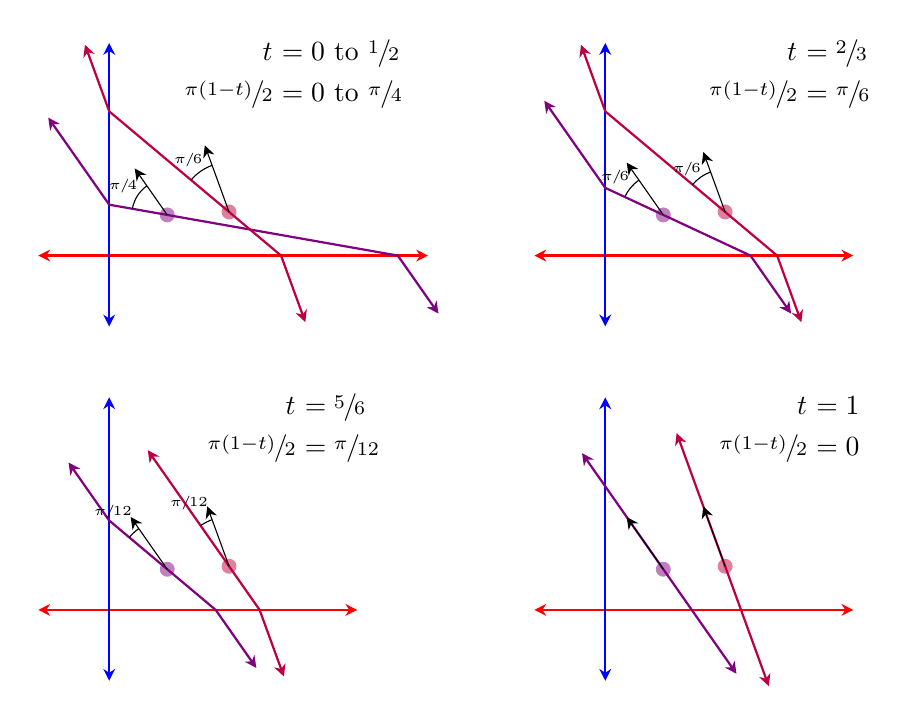
\begin{tikzpicture}[scale=.9]
\let\frac\sfrac
\let\tfrac\sfrac
\begin{scope}[shift={(-7,0)}]

\draw[thick,red,<->]
(-1,0) -- (4.5,0);
\draw[thick,blue,<->]
(0,-1) -- (0,3);
\path
(0,0) coordinate (o);

\def\A{-55}
\def\B{-10}

\fill[violet!50]
({\A+90}:1) coordinate (q0) circle (3pt);
\path
(q0) ++(\B:2) coordinate (a)
(o) ++(3,0) coordinate (b)
(intersection of q0--a and o--b) coordinate (p2) ++(\A:1) coordinate (p1b)
(q0) ++(\B:-2) coordinate (a)
(o) ++(0,3) coordinate (b)
(intersection of q0--a and o--b) coordinate (p3) ++(\A:-1.5) coordinate (p1a)
;
\draw[thick,violet,<->]
(p1a) -- (p3) -- (p2) -- (p1b);
\draw[thin,->]
(q0) ++(\B:-.5) arc ({\B-180}:{\A-180}:.5) node[left] {\tiny $\tfrac{\pi}{4}$}
(q0) -- ++(\A:-.8)
;

\def\A{-70}
\def\B{-40}

\fill[purple!50]
({\A+90}:1.8) coordinate (q0) circle (3pt);
\path
(q0) ++(\B:2) coordinate (a)
(o) ++(3,0) coordinate (b)
(intersection of q0--a and o--b) coordinate (p2) ++(\A:1) coordinate (p1b)
(q0) ++(\B:-2) coordinate (a)
(o) ++(0,3) coordinate (b)
(intersection of q0--a and o--b) coordinate (p3) ++(\A:-1) coordinate (p1a)
;
\draw[thick,purple,<->]
(p1a) -- (p3) -- (p2) -- (p1b);
\draw[thin,->]
(q0) ++(\B:-.7) arc ({\B-180}:{\A-180}:.7) node[left,shift={(0,2pt)}] {\tiny $\tfrac{\pi}{6}$}
(q0) -- ++(\A:-1)
;

\node at (2.5,2.5) {$\begin{array}{r@{\ }l@{\vspace{3pt}}} t &=0 \text{ to } \frac{1}{2} \\ \frac{\pi(1{-}t)}{2} &=0 \text{ to } \frac{\pi}{4} \end{array}$};

\end{scope}

\begin{scope}[shift={(0,0)}]

\draw[thick,red,<->]
(-1,0) -- (3.5,0);
\draw[thick,blue,<->]
(0,-1) -- (0,3);
\path
(0,0) coordinate (o);

\def\A{-55}
\def\B{-25}

\fill[violet!50]
({\A+90}:1) coordinate (q0) circle (3pt);
\path
(q0) ++(\B:2) coordinate (a)
(o) ++(3,0) coordinate (b)
(intersection of q0--a and o--b) coordinate (p2) ++(\A:1) coordinate (p1b)
(q0) ++(\B:-2) coordinate (a)
(o) ++(0,3) coordinate (b)
(intersection of q0--a and o--b) coordinate (p3) ++(\A:-1.5) coordinate (p1a)
;
\draw[thick,violet,<->]
(p1a) -- (p3) -- (p2) -- (p1b);
\draw[thin,->]
(q0) ++(\B:-.6) arc ({\B-180}:{\A-180}:.6) node[left,shift={(0,1pt)}] {\tiny $\tfrac{\pi}{6}$}
(q0) -- ++(\A:-.9)
;

\def\A{-70}
\def\B{-40}

\fill[purple!50]
({\A+90}:1.8) coordinate (q0) circle (3pt);
\path
(q0) ++(\B:2) coordinate (a)
(o) ++(3,0) coordinate (b)
(intersection of q0--a and o--b) coordinate (p2) ++(\A:1) coordinate (p1b)
(q0) ++(\B:-2) coordinate (a)
(o) ++(0,3) coordinate (b)
(intersection of q0--a and o--b) coordinate (p3) ++(\A:-1) coordinate (p1a)
;
\draw[thick,purple,<->]
(p1a) -- (p3) -- (p2) -- (p1b);
\draw[thin,->]
(q0) ++(\B:-.6) arc ({\B-180}:{\A-180}:.6) node[left,shift={(0,1pt)}] {\tiny $\tfrac{\pi}{6}$}
(q0) -- ++(\A:-.9)
;

\node at (2.5,2.5) {$\begin{array}{r@{\ }l@{\vspace{3pt}}} t &=\frac{2}{3} \\ \frac{\pi(1{-}t)}{2} &=\frac{\pi}{6} \end{array}$};

\end{scope}

\begin{scope}[shift={(-7,-5)}]

\draw[thick,red,<->]
(-1,0) -- (3.5,0);
\draw[thick,blue,<->]
(0,-1) -- (0,3);
\path
(0,0) coordinate (o);

\def\A{-55}
\def\B{-40}

\fill[violet!50]
({\A+90}:1) coordinate (q0) circle (3pt);
\path
(q0) ++(\B:2) coordinate (a)
(o) ++(3,0) coordinate (b)
(intersection of q0--a and o--b) coordinate (p2) ++(\A:1) coordinate (p1b)
(q0) ++(\B:-2) coordinate (a)
(o) ++(0,3) coordinate (b)
(intersection of q0--a and o--b) coordinate (p3) ++(\A:-1) coordinate (p1a)
;
\draw[thick,violet,<->]
(p1a) -- (p3) -- (p2) -- (p1b);
\draw[thin,->]
(q0) ++(\B:-.7) arc ({\B-180}:{\A-180}:.7) node[above left,shift={(1pt,0)}] {\tiny $\tfrac{\pi}{12}$}
(q0) -- ++(\A:-.9)
;

\def\A{-70}
\def\B{-55}

\fill[purple!50]
({\A+90}:1.8) coordinate (q0) circle (3pt);
\path
(q0) ++(\B:2) coordinate (a)
(o) ++(3,0) coordinate (b)
(intersection of q0--a and o--b) coordinate (p2) ++(\A:1) coordinate (p1b)
(q0) ++(\B:-2) coordinate (a)
;
\draw[thick,purple,<->]
(a) -- (p2) -- (p1b);
\draw[thin,->]
(q0) ++(\B:-.7) arc ({\B-180}:{\A-180}:.7) node[above left,shift={(2pt,0)}] {\tiny $\tfrac{\pi}{12}$}
(q0) -- ++(\A:-.9)
;

\node at (2.5,2.5) {$\begin{array}{r@{\ }l@{\vspace{3pt}}} t &=\frac{5}{6} \\ \frac{\pi(1{-}t)}{2} &=\frac{\pi}{12} \end{array}$};

\end{scope}

\begin{scope}[shift={(0,-5)}]
\draw[thick,red,<->]
(-1,0) -- (3.5,0);
\draw[thick,blue,<->]
(0,-1) -- (0,3);
\path
(0,0) coordinate (o);

\def\A{-55}

\fill[violet!50]
({\A+90}:1) coordinate (q0) circle (3pt);
\path
(q0) ++(\A:1.8) coordinate (a)
(q0) ++(\A:-2) coordinate (b)
;
\draw[thick,violet,<->]
(a) -- (b);
\draw[thin,->]
(q0) -- ++(\A:-.9)
;

\def\A{-70}

\fill[purple!50]
({\A+90}:1.8) coordinate (q0) circle (3pt);
\path
(q0) ++(\A:1.8) coordinate (a)
(q0) ++(\A:-2) coordinate (b)
;
\draw[thick,purple,<->]
(a) -- (b);
\draw[thin,->]
(q0) -- ++(\A:-.9)
;

\node at (2.5,2.5) {$\begin{array}{r@{\ }l@{\vspace{3pt}}} t &=1 \\ \frac{\pi(1{-}t)}{2} &=0 \end{array}$};

\end{scope}

\end{tikzpicture}

\caption{An example of the deformation $h_I$ for $m=3$.}
\label{figure-hI3}

\end{center}

\end{figure}

\begin{claim}\label{claim-lambda-def-3}
For $m =3$, $\lambda(t)$ is well-defined and is a pseudoline extension of $L_{i_1},L_{i_2},L_{i_3}$.
\end{claim}

\begin{proof}
Assume that we are in the case where $\lambda(0)$ is not straight and that \hbox{$(\nicefrac{\pi}{2})(1-t) < |\delta|$}, since the claim is trivial otherwise.
We may assume by symmetry that $p_3(0)$ is above the origin on the vertical axis, and $p_2(0)$ is to the right of the origin on the horizontal axis.

We show that $q_0$ is well-defined and is on the segment between $p_2(0)$ and $p_3(0)$.
By our assumption, $\lambda(0)$ is an implicit function with a finite negative slope in the upper-right quadrant.
Also, our assumption implies that $\lambda(0)$ is unbounded on $\mb{R}^2$ in the upper-left and lower-right quadrants, and $\lambda(0)$ is neither vertical nor horizontal there since $p_1$ is not on $L_{i_2}$ or $L_{i_3}$, so $\lambda(0)$ is an implicit function with a finite negative slope in both of these quadrants as well.
Since lines through $p_1$ have finite negative slope, $P$ is an implicit function with a finite positive slope, and therefore, $\lambda(0)$ and~$P$ meet at a unique point $q_0$ in the upper-right quadrant, so the point $q_0$ is between $p_2(0)$ and $p_3(0)$ on $\lambda(0)$.

Any line through $q_0$ with finite negative slope intersects $L_{i_2}$ in $\mb{R}^2$ to the right of the origin and intersects $L_{i_3}$ in $\mb{R}^2$ above the origin.
Therefore, the points $p_2(t)$ and $p_3(t)$ move along $L_{i_2}$ and $L_{i_3}$ respectively without crossing the origin or leaving the plane.
Hence, $\lambda(t)$ is a well-defined path consisting of a segment in the upper-left, upper-right, and lower-right quadrants each.
Furthermore, we now have that $\lambda(t)$ crosses $L_{i_1}$, $L_{i_2}$, and $L_{i_3}$ once each, so this is a pseudoline arrangement.
\end{proof}

\begin{claim}\label{claim-lambda-continuous-3}
For $m =3$, $\tilde \lambda$ is continuous on the domain where it is defined. Hence, $\tilde \lambda$ is an extension deformation process on $\tilde Z_I$.
\end{claim}

\begin{proof}
For $j \in \{1,\dots,\infty\}$, let $\lambda_j(t)$ be as above and $t_j \in [0,1]_\mb{R}$ such that $\lambda_j(0) \to \lambda_\infty(0)$ and $t_j \to t_\infty$.
Recall that we use the metric on $\projplane$ induced from Fréchet distance on the sphere.

If $\lambda_j(0)$ is straight for all $j \in \mb{N}$ large enough, then $\lambda_j(t) = \lambda_j(0) \to \lambda_\infty(0) = \lambda_\infty(t')$ and we are done.
Otherwise we may restrict to a subsequence that is not straight.
Therefore, assume that $\lambda_j(0)$ is not a straight line for $j\neq \infty$.

Let $p_{1,j}$, $p_{2,j}(t)$, $p_{3,j}(t)$, $P_j$, $q_{0,j}$, and $Q_{j}(t)$ be defined as above for $j < \infty$ and also for $j=\infty$ where appropriate.

We have four cases to consider, $\lambda_\infty(0)$ intersects $L_{i_1},L_{i_2},L_{i_3}$ at $3$ distinct points, or $\lambda_\infty(0)$ is vertical or horizontal, or $\lambda_\infty(0)$ is a straight line through the origin that is neither vertical nor horizontal, or $\lambda_\infty(0) = L_{i_1}$ is the horizon.

Suppose that $\lambda_\infty(0)$ intersects $L_{i_1},L_{i_2},L_{i_3}$ at $3$ distinct points. Then by Lemma \ref{lemma-vertex}, we have $p_{k,j}(0) \to p_{k,\infty}(0)$, so $q_{0,j} \to q_{0,\infty}$, so $\lambda_j(1) \to \lambda_\infty(1)$, so $Q_{j}(t_j) \to Q_{\infty}(t_\infty)$, so $p_{k,j}(t_j) \to p_{k,\infty}(t_\infty)$, so $\lambda_j(t_j) \to \lambda_\infty(t_\infty)$ since these are defined continuously in terms of each other in succession.

Suppose that $\lambda_\infty(0)$ is vertical. Then, $p_1$ and $p_{3,j}(0)$ both converge to $(L_{i_1} \cap L_{i_3})$, so $P_j \to L_{i_2}$, so $q_{0,j} \to p_{2,\infty}(0) = (\lambda_\infty(0) \cap L_{i_2})$, so $\lambda_j(t_j)$ converges to the vertical line through $p_{2,\infty}(0)$, which is $\lambda_\infty(t_\infty) = \lambda_\infty(0)$.
The argument for $\lambda_\infty(0)$ horizontal is essentially the same.

Suppose that $\lambda_\infty(0)$ contains the origin and is neither vertical nor horizontal. Then, $p_{2,j}(0) \to 0$ and $p_{3,j}(0) \to 0$, so $q_{0,j} \to 0$. Since $p_{1,j} \to p_{1,\infty} = (\lambda_\infty(0) \cap L_{i_1})$, we have $p_{1,j}$ bounded away from $L_{i_2}$ and $L_{i_3}$ for $j$ large enough, so $p_{k,j}(1) \to 0$ for $k \in \{2,3\}$. Since $p_{k,j}(t_k)$ is on $L_{i_k}$ between $p_{k,j}(0)$ and $p_{k,j}(1)$ in $\mb{R}^2$, we have $p_{k,j}(t_j) \to 0$, so $\lambda_j(t_j)$ converges to the line through the origin and $p_{1,\infty}$, which is $\lambda_\infty(t_\infty) = \lambda_\infty(0)$.

Suppose that $\lambda_\infty(0)$ is the horizon.
Then, $\min \{\|x\| : x \in \lambda_j(0)\} \to \infty$, so
although $q_{0,j}$ might not converge, $\|q_{0,j}\| \to \infty$.
Since $q_{0,j} = (P_{j} \cap \lambda_j(1))$, and $P_{j}$ and $\lambda_j(1)$ are perpendicular, we have $\min \{\|x\| : x \in \lambda_j(1)\} = \|q_{0,j}\| \to \infty$.
Since~$\lambda_j(t)$ pivots about the point $q_{0,j}$ in one quadrant, and is parallel in two other quadrants, $\lambda_j(t_j)$ is separated from the origin by the lower envelope of $\lambda_j(0)$ and $\lambda_j(1)$, so~\hbox{$\min \{\|x\| : x \in \lambda_j(t_j)\} \to \infty$}, which means $\lambda_j(t_j)$ converges to the horizon.
\end{proof}

Let $\Lambda(A,t) = \bigl(\tilde \lambda(\tilde A,L_1,t),\dots,\tilde \lambda(\tilde A,L_n,t)\bigr)$.

\begin{claim}\label{claim-lambda-arrangement-3}
For $m=3$, $\Lambda(A,t)$ is a pseudoline arrangement. Hence, $h_I$ is a~well-defined $\orth_3$-equivariant deformation of $Z_I$.
\end{claim}

\begin{proof}
Let $\lambda_j(t)=\tilde \lambda(\tilde A, L_j,t)$, and again let $p_{1,j}$, $p_{2,j}(t)$, $p_{3,j}(t)$, $P_j$, $q_{0,j}$, and $\phi_j(t)$ be defined for $\lambda_j$ as above.

Assume for the sake of contradiction that $\Lambda(A,t)$ is not a pseudoline arrangement for some $t\in [0,1]_\mb{R}$, and let $t_0$ be the infimum of such $t$.
Then, there is a pair $\lambda_j,\lambda_\xj$ and a sequence $t_k \to t_0$ from above where the conditions defining a pseudoline arrangement are violated.
That is, $\lambda_j(t_k)$ and $\lambda_\xj(t_k)$ intersect at more than 1 point, but do not coincide.

We claim that $\lambda_j(t)$ and $\lambda_\xj(t)$ never coincide. If there were $t'$ such that $\lambda_j(t')=\lambda_\xj(t')$ coincide, then we would have $p_{1,j}(t') = p_{1,\xj}(t')$, so $p_{1,j}(0) = p_{1,\xj}(0)$ since $p_{1,j}$ remains constant throughout the deformation.
Similarly, $q_{0,j}(0) = q_{0,\xj}(0)$ since $q_{0,j}$ also remains constant.
Since $\Lambda(A,0)$ is a pseudoline arrangement and $\lambda_j(0)$ and $\lambda_\xj(0)$ intersect at more than one point, we must have $\lambda_j(0) = \lambda_\xj(0)$, which implies that $\lambda_j(t) = \lambda_\xj(t)$ throughout the deformation, but this contradicts that the pair $\lambda_j,\lambda_\xj$ eventually fail to be a pseudoline arrangement.
Thus, $\lambda_j(t)$ and $\lambda_\xj(t)$ never coincide,
which implies that $\lambda_j(t)$ and $\lambda_\xj(t)$ meet at a single point for all $t<t_0$, which we denote by $x(t)$.

If both pairs of points $p_{i,j}(t_0),p_{i,\xj}(t_0)$ for $i \in \{2,3\}$ were distinct, then $\lambda_j(t)$ and $\lambda_\xj(t)$ would meet at the same number of points for $t$ before and after~$t_0$ for~$t$ sufficiently close to $t_0$ which contradicts that $\lambda_j,\lambda_\xj$ is a pseudoline arrangement before~$t_0$ but fails to be a pseudoline arrangement at $t_k \to t_0$ from above.
We may assume by symmetry that $p_{2,j}(t_0) = p_{2,\xj}(t_0)$ and denote this point by $y$.

If $y$ were a limit point of $x(t)$
and $p_{3,j}(t_0) \neq p_{3,\xj}(t_0)$, then $x(t)$ would have to converge to $y$, and again we would have that $\lambda_j(t)\cap \lambda_\xj(t)$ is a single point for all $t$ sufficiently close to $t_0$, which is a contradiction. Hence, for one of these pairs of vertices, the vertices must coincide with each other and be bounded away from $x(t)$.
Let us also assume by symmetry that $x(t)$ is bounded away from $y = p_{2,j}(t_0) = p_{2,\xj}(t_0)$ as $t \to t_0$ from below.

If the exterior angles of $\lambda_j(t_0)$ and $\lambda_\xj(t_0)$ at $y$ were equal, then either $\lambda_j(t_0),\lambda_\xj(t_0)$ would cross at $y$, which would contradict that $y$ is bounded away from $x(t)$, or $\lambda_j(t_0),\lambda_\xj(t_0)$ would coincide along the segments on both sides of $y$, which would imply $p_{1,j} = p_{1,\xj}$ and $q_{0,j} = q_{0,\xj}$, so $\lambda_j(0) = \lambda_\xj(0)$, which is impossible.
Therefore, we may assume by symmetry that the exterior angle of $\lambda_j(t_0)$ at $y$ is strictly greater than that of $\lambda_\xj(t_0)$. Thus, $\lambda_j(t)$ has already begun deforming by time $t=t_0$, while $\lambda_\xj(t)$ has been fixed up to time $t_0$.

Let $C_j(t)$ be the cone emanating from $p_{2,j}(t)$ generated by the segments of $\lambda_j(t)$ incident to $p_{2,j}(t)$, and let $C_\xj(t)$ be defined analogously.
Since the exterior angle of $\lambda_j(t_0)$ at $y$ is strictly greater than that of $\lambda_\xj(t_0)$, the interior angle of $\lambda_j(t_0)$ is strictly less than that of $\lambda_\xj(t_0)$, and $\lambda_j(t_0),\lambda_\xj(t_0)$ do not cross at $y$, so at $t_0$ the cones are nested, \ie $C_j(t_0) \subset C_\xj(t_0)$.

The vertex $p_{2,j}(t)$ moves along the horizontal axis $L_{i_2}$ in the direction toward the interior of the cone $C_j(t)$, so for $t < t_0$, the apex $p_{2,j}(t)$ of $C_j(t)$ is outside of $C_j(t_0)$. The cones $C_j(t)$ and $C_\xj(t)$ straddle $L_{i_2}$ in the same direction, so $p_{2,j}(t)$ is also outside of $C_\xj(t)= C_\xj(t_0)$, and the interior angle of $C_j(t)$ is smaller than that of $C_\xj(t)$, so~the boundaries of the cones intersect.
This intersection approaches $y$ as $t\to t_0$ from below, so the point $\lambda_j(t)\cap \lambda_\xj(t)$ approaches $y$, which is a contradiction.
Thus, $\Lambda(A,t)$ must be a pseudoline arrangement throughout the deformation.
\end{proof}

\begin{claim}\label{claim-deform-h3}
$h_{(i_1,i_2,i_3)}$ is a strong $\orth_3$-equivariant deformation retraction from $Z_{(i_1,i_2,i_3)}$ to $Z_{(i_1,i_2)} = Z_{()}$.
\end{claim}

\begin{proof}
Since $\lambda_j(t)$ is geodesic in each cell of $L_{i_1},L_{i_2},L_{i_3}$ throughout the deformation, we have $h_I(t) \in Z_I$, and since $\lambda_j(1)$ is a line, we have $h_I(1) \in Z_{()}$.
Therefore, $h_I$ is a deformation retraction from $Z_I$ to $Z_{()}$.
Since $\lambda$ is the trivial deformation if $\lambda(0)$ is a line, $h_I$ is a strong deformation retraction.
\end{proof}

Recall that for $m < 3$, $h_I(A,t) = A$ is trivial.

\begin{claim}\label{claim-stable-h}
For all $p \in \{0,\dots,m{-}1\}$ and all $j \in [n]_\mb{N} \setminus \{i_1,\dots,i_p\}$,
if $A \in Z_I \cap X_{(i_1,\dots,i_{p},j)}$ then $h_I(A,1) \in X_{(i_1,\dots,i_{p},j)}$.
\end{claim}

\begin{proof}
For $p = 0$ or $p \geq 3$, the claim holds since the deformation $h_I$ preserves norms.
For $p = 1$, if $S_{i_1}$ and $S_j$ are distinct, then they remain distinct throughout the deformation, so the claim holds.
For $p = 2$ and $m > 3$, the pseudocircle $S_j$ can only deform in interiors of $2$-cells of $S_{i_1},\dots,S_{i_m}$, so the intersections of $S_j$ with $S_{i_1}$ and with $S_{i_2}$ are preserved throughout the deformation, so the claim holds.
For $p = 2$ and $m = 3$, the intersection of $\lambda(t)$ with $L_{i_1}$ is fixed throughout the deformation, so the points where $S_{i_2}$ and $S_j$ meet $S_{i_1}$ are preserved throughout the deformation, so the claim holds.
\end{proof}

\subsection{The deformation $g_I$ from $Y_I$ to $Z_I$ for $n < \infty$}
\label{subsubsec-g-finite}

Let $(\cdot)$ denote the operation augmenting a sequence, $(x_1, \dots, x_k) \cdot y = (x_1, \dots, x_k, y)$.
Let this also denote concatenation of deformations,
\[\phi_2 \cdot \phi_1 (x,t) =
\begin{cases}
\phi_1(x,\, 2t) & t \in [0, \nicefrac{1}{2}]_\mb{R}, \\
\phi_2(\phi_1(x,1),\, 2t{-}1) & t \in [\nicefrac{1}{2},1]_\mb{R}, \\
\end{cases}
\]
with composition left associative. Note that $\phi_2$ must be a deformation of the range of $\phi_1$ at $t=1$.
We use $\prod_{j \in J} \phi_j$ to denote the concatenation of the deformations $\phi_j$ for $j \in J \subseteq \mb{N}$ in increasing order from right to left.
In this subsection $J$ will always be finite.

We next define the deformations $g_I$ using the $f_I$ and $h_I$.
Here we assume that $n \in \{3,\dots\}$. The infinite case will be dealt with in the next subsection.

Our situation so far is this.
If we were only concerned with the space of arrangements where none of the weighted pseudocircles vanish, and the first three $\alpha_1,\alpha_2,\alpha_3$ are always a basis, then we could straighten all pseudocircles with the deformation given by
\begin{equation}\label{deformation-naive}
h_{(1)} \cdot h_{(1,2)} \cdots h_{(1,\dots,n)} \cdot f_{(1,\dots,n)} \cdots f_{(1,2)} \cdot f_{(1)},
\end{equation}
but these assumptions only hold on some proper subset of $\pstief_{3,n}$.
What we need is a deformation retraction from $Y_{()} = \pstief_{3,n}$ to $Z_{()}$.
Moreover, $f_{(1,\dots,{m-1})}$ is a defor\-mation retraction to $Y_{(1,\dots,{m-1})}$, and the next deformation we would like to use, namely $f_{(1,\dots,m)}$, is only defined on $X_{(1,\dots,m)}$, which is a proper subset of $Y_{(1,\dots,{m-1})}$.
Even worse, the spaces $X_{I\cdot j}$ for $j \not\in I$ do not even cover $Y_I$.
To deal with this, we will use the fact that these deformations approach the trivial deformation near the complement of the union of the $X_{I\cdot j}$.
Let
\[ U_I = \bigcup_{j\in\compl{I}} X_{I\cdot j}
=\{ (\alpha_1,\dots,\alpha_n) \in Y_I:\exists j \in \compl{I}.\ \|\alpha_j\| > 0\}. \]
Note that the second equality above holds by definition of $X_I$ for $m \geq 3$, and holds by the fact that every $A \in \pstief_{3,n}$ has a basis for $m <3$.
Moreover, since every independent set can be completed to a basis, we have that $U_I = Y_I$ for $m < 3$.

We will also continuously shift between the deformations corresponding to different sequences of indices by stopping certain deformations early.
For spaces $X \subseteq Y$, \hbox{$s \in [0,1]_\mb{R}$}, and a homotopy $\phi:X \times [0,s]_\mb{R} \to Y$ defined at least up to time $s$, let
\[ \upto(\phi,s) : X \times [0,1]_\mb{R} \to Y, \quad \upto(\phi,s;x,t) = \phi(x,\min(s,t)). \]
That is, $\upto(\phi,s)$ is the deformation of $X$ that coincides with $\phi$ up to the stopping time $s$ and then remains fixed thereafter.
We allow $\upto(\phi,0)$ to be the trivial deformation even for input that is outside the domain of $\phi$.
That is, we let $\upto(\phi,0; y,t) = y$ for $y \in Y$.

We may be tempted to order the set of all permutations of $[n]_\mb{N}$, and deform an initial arrangement $A$ as in deformation (\ref{deformation-naive}) using each permutation one at a time, but stopping early for certain permutations, so that we do not have to deform $A$ using a permutation that will not work. The problem with this, is that a permutation that would have worked initially for $A$ might no longer work after $A$ has been deformed using another permutation. To deal with this, we define deformation retractions $g_I$ from $Y_I$ to $Z_I$ recursively as follows. Our desired deformation will then be $g_{()}$.
Recall $m=|I|$.
If $m=n$, then $g_I$ is just the trivial deformation $g_I({A},t) = {A}$.
Otherwise for $m<n$, $g_I$ is defined recursively by
\begin{equation}\label{equation-g}
g_{I}({A},t) = \biggl( \prod_{j \in \compl{I} } \upto\left(h_{I \cdot j} \cdot g_{I \cdot j} \cdot f_{I \cdot j},\ s_{I \cdot j} ({A}) \right)\biggr) ({A},t),
\end{equation}
where $s_{I \cdot j}$ is defined for $j \in \compl{I}$ as follows,
\begin{align*}
r_{I\cdot j}(A) &= \inf \left\{\dist(B,A): B \in Y_{I} \setminus X_{I\cdot j} \right\},\\
s_{I \cdot j}(A) &= \begin{cases}
0 & A \not\in U_{I}, \\
\biggl(2\biggl(\frac{\displaystyle r_{I\cdot j}({A})}{\displaystyle \max_{k \in \compl{I}} r_{I\cdot k}({A}) }\biggr) -1 \biggr)^+ & A \in U_{I}, \\
\end{cases}
\end{align*}
and where $(\phi(x))^+ = \max(0,\phi(x))$ is the positive part of a function $\phi$.

Here, we let $\upto\left(h_{I \cdot j} \cdot g_{I \cdot j} \cdot f_{I \cdot j},\ s \right)$ be the trivial deformation on all of $Y_I$ when $s=0$. Note that if $s > 0$, then this deformation is only defined on $X_{I\cdot j}$.

\begin{claim}\label{claim-s}
For all $A \in Y_I$ and $j \in \compl{I}$, $s_{I\cdot j}(A)$ is well-defined, and $s_{I\cdot j}$ is continuous on $U_{I}$.
\end{claim}

Note that $s_{I\cdot j}$ is not continuous on all of $Y_I$.

\begin{proof}
If $A \not\in U_{I}$, then $s_{I\cdot j}(A)=0 $ is well-defined.
Alternatively, if $A \in U_{I}$, then there is some $j_0 \in \compl{I}$ such that $A \in X_{I\cdot j_0}$, which implies that $r_{I\cdot j_0}(A) > 0$ by Claim~\ref{claim-open-X}.
Therefore, $\max_{k \in \compl{I}} r_{I\cdot k}({A}) > 0$, which implies that $s_{I\cdot j}(A)$ is well-defined for all $j \in \compl{I}$.

For the second part, observe that distance to a closed set in a metric space is continuous, so each $r_{I\cdot j}$ is continuous on $Y_I$. We have that $\max_{k \in \compl{I}} r_{I\cdot k}(A)$ is strictly positive on $A \in U_I$, so $(\max_{k \in \compl{I}} r_{I\cdot k}(A))^{-1}$ is continuous there, which implies that~$s_{I\cdot j}$ is continuous on $U_I$.
\end{proof}

\begin{claim}\label{claim-g}
$g_I$ is a well-defined strong equivariant deformation retraction from~$Y_I$ to $Z_I$.

Moreover, let $\compl{I} = \{j_1,\dots,j_{n-m}\}$ and for $e \in \{0,\dots,n-m\}$ let
\[ \tilde g_{I, e}({A},t) = \biggl( \prod_{j =j_1}^{j_e} \upto\left(h_{I \cdot j} \cdot g_{I \cdot j} \cdot f_{I \cdot j},\ s_{I \cdot j} ({A}) \right) \biggr) ({A},t) \]
be the initial part of the deformation $g_I$ up to the $e$-th element of $\compl{I}$.
For all $A \in Y_I$, $t \in [0,1]_\mb{R}$, and $e \in \{0,\dots,n{-}m\}$, we have the following.

\vbox{
\begin{enumerate}
\item\label{part-g-defined}
$\tilde g_{I, e}(A,t) \in Y_I$ is well-defined and equivariant.
\item\label{part-g-continuous}
$\tilde g_{I, e}$ is continuous.
\item\label{part-g-strong}
If $A \in Z_I$, then $\tilde g_{I,e}(A,t) =A$ is the trivial deformation.
\item\label{part-g-stable}
For all $p \in \{0,\dots,m\}$ and $j \in [n]_\mb{N} \setminus \{i_1,\dots,i_{p}\}$,
if $A \in X_{(i_1,\dots,i_{p},j)}$ then $\tilde g_{I,e}(A,1) \in X_{(i_1,\dots,i_{p},j)}$.
\item\label{part-g-proj}
$\proj_I(\tilde g_{I,e}({A},t)) = \proj_I({A})$, and $\tilde g_{I,e}$ preserves norms.
\end{enumerate}
}
\end{claim}

\begin{proof}
We proceed by nested induction arguments on $m$ decreasing from $m=n$ and on $e$ increasing from $e=0$. To show continuity, we consider $A_k \to A$ and $t_k \to t$.

For $m = n$, $g_I$ is just the trivial deformation and $Z_I = Y_I$, so the claim holds. Let $m < n$. Our first inductive assumption is that for all $j\in \compl{I}$, the claim holds for $g_{I\cdot j} = \tilde g_{I\cdot j,n-m-1}$.

Also for $e=0$, $\tilde g_{I,e}$ is just the trivial deformation, so the parts of the claim for $\tilde g_{I,e}$ hold.
Let $e > 0$, and let $A' = \tilde g_{I,e-1}(A,1)$. Our second inductive assumption is that the claim holds for $\tilde g_{I,e-1}$.

\subsubsection*{Suppose first that $A \in X_{I\cdot j_e}$}

We start by showing parts \eqref{part-g-defined}, \eqref{part-g-strong}, and \eqref{part-g-proj}.
Here is the crucial reason why we need part~\eqref{part-g-stable} of the claim to show that $g_I$ is well-defined: by the second inductive assumption for part~\eqref{part-g-stable} of the claim, we have that $A' \in X_{I\cdot j_e}$. This implies that $f_{I\cdot j_e}(A',t) \in X_{I\cdot j_e}$ is well-defined, equivariant, and trivial on $Y_{I\cdot j_e}$ by Claim~\ref{claim-deform-f3} for $m=3$ and Claim~\ref{claim-deform-f} for $m>3$, and $f_{I\cdot j_e}(A',1) \in Y_{I\cdot j_e}$.
Therefore, $g_{I\cdot j_e} \cdot f_{I\cdot j_e}(A',t) \in Y_{I\cdot j_e}$ is well-defined, equivariant, and trivial on $Z_{I\cdot j_e}$ by the first inductive assumption, and $g_{I\cdot j_e} \cdot f_{I\cdot j_e}(A',1) \in Z_{I\cdot j_e}$, so $h_{I\cdot j_e}\cdot g_{I\cdot j_e}\cdot f_{I\cdot j_e}(A',t) \in Z_{I\cdot j_e}$ is well-defined, equivariant, and trivial on $Z_I$ by Claims~\ref{claim-deform-h} and \ref{claim-deform-h3}.
Recall that $Z_I \subset Z_{I\cdot j_e} \subseteq Y_{I\cdot j_e} \subset X_{I\cdot j_e} \subset Y_I$, so $\tilde g_{I, j_1}({A},t) \in Y_I$ is well-defined, equivariant, and trivial on $Z_I$, which means parts~\eqref{part-g-defined} and~\eqref{part-g-strong} hold.
Similarly, we have part~\eqref{part-g-proj} by the inductive assumptions and the definitions of $f_{I\cdot j_e}$ and $h_{I\cdot j_e}$.

Next we show part \eqref{part-g-stable}.
Consider now the case where $A \in X_{(i_1,\dots,i_{p},j)}$.
Again, $A' \in X_{(i_1,\dots,i_{p},j)}$ by the second inductive assumption, so $f_{I\cdot j_e}(A',1) \in X_{(i_1,\dots,i_{p},j)}$ by Claim~\ref{claim-stable-f}, and so $g_{I\cdot j_e}\cdot f_{I\cdot j_e}(A',1) \in X_{(i_1,\dots,i_{p},j)}$ by the first inductive assumption, and so $h_{I\cdot j_e}\cdot g_{I\cdot j_e}\cdot f_{I\cdot j_e}(A',1) \in X_{(i_1,\dots,i_{p},j)}$ by Claim~\ref{claim-stable-h}.
Thus, part~\eqref{part-g-stable} holds.

Next we show part \eqref{part-g-continuous}.
By the second inductive assumption, we have $A'_k = g_{I,e-1}(A,1) \to A' \in X_{I\cdot j_e}$.
Since $X_{I\cdot j_e}$ is an open subset of $Y_I$ by Claim~\ref{claim-open-X}, $A'_k \in X_{I\cdot j_e}$ for $k$ sufficiently large, and since $f_{I\cdot j_e}$ is continuous on $X_{I\cdot j_e}$, we have $f_{I,e}(A'_k,t_k) \to f_{I,e}(A',t)$.
Since $g_{I\cdot j_e}$, $h_{I\cdot j_e}$, and $s_{I\cdot j_e}$ are respectively continuous on $Y_{I\cdot j_e}$, $Z_{I\cdot j_e}$, and $U_{I} \supset X_{I\cdot j_e}$, we have that $\tilde g_{I,e}$ is continuous. Thus, part~\eqref{part-g-continuous} holds.

\subsubsection*{Suppose next that $A \not\in X_{I\cdot j_e}$}

Then, $s_{I\cdot j_e}(A) = 0$, so $\tilde g_{I,e}(A,t)$ is the concatenation of $\tilde g_{I,e-1}(A,t)$ with a trivial deformation.
Specifically, $\tilde g_{I,e}(A,t) = \tilde g_{I,e-1}(A,\tau(t))$, where $\tau(t) = \min(2t,1)$
is a non-decreasing surjective transformation of the unit interval, which means that parts \eqref{part-g-defined}, \eqref{part-g-strong}, \eqref{part-g-stable}, and \eqref{part-g-proj} hold by the second inductive assumption. It remains to show part \eqref{part-g-continuous} in this case.

Suppose also that $A \in U_I$. Then, there is some $j$ such that $A \in X_{I\cdot j}$, so $r_{I\cdot j}(A_k)$ is bounded below by some $r > 0$ for $k$ sufficiently large, whereas $r_{I\cdot j_e}(A_k) \to 0$, which implies that $s_{I\cdot j_e}(A_k) = 0$ for $k$ sufficiently large. Therefore, $\tilde g_{I,e}(A_k,t_k) = \tilde g_{I,e-1}(A_k,\tau(t_k))$, so part~\eqref{part-g-continuous} holds.

Suppose instead that $A \not\in U_I$.
This implies that for all $j \in \compl{I}$, $s_{I\cdot j}(A) = 0$, so $\tilde g_{I\cdot e}(A,t) = A$.
Since every $A \in \pstief_{3,n}$ includes a basis among its elements, and any independent set can be completed to a basis, we have $U_I = Y_I$ for $m \leq 2$. Therefore, we must have $m \geq 3$ in this case, which means that each of the $X_{I\cdot j}$ consists of the weighted pseudocircle arrangements in $Y_I$ where the $j$-th element does not vanish. Since $A$ is in none of the $X_{I\cdot j}$, we have $\proj_I(A) = A$, which implies that $\proj_I(A_k) \to A$.
We have already shown that part~\eqref{part-g-proj} of the claim holds for $\tilde g_{I,e}(A_k,t_k)$ (in both cases $A_k \not\in X_{I\cdot j_e}$ and $A_k \in X_{I\cdot j_e}$), so $\proj_I(\tilde g_{I,e}(A_k,t_k)) = \proj_I(A_k)$ and $\tilde g_{I,e}$ preserves norms. Therefore, for all $j \in \compl{I}$, the $j$-th element of $\tilde g_{I,e}(A_k,t_k)$ converges to 0, since the $j$-th element of $A_k$ converges to 0. This implies that \[ \dist(\tilde g_{I,e}(A_k,t_k),\proj_I(A_k)) = \dist(\tilde g_{I,e}(A_k,t_k),\proj_I(\tilde g_{I,e}(A_k,t_k))) \to 0, \]
so $\tilde g_{I,e}(A_k,t_k) \to A = \tilde g_{I\cdot e}(A,t)$.
Thus, part~\eqref{part-g-continuous} holds.

This completes the induction on $e$.
So far we have established all 5 conditions on $\tilde g_{I\cdot e}$.
It remains to show that $g_I(A,1) \in Z_I$.

If $A \not\in U_I$, then we must have $m \geq 3$, which means $\alpha_j = 0$ for all $j \in \compl{I}$, so~$A \in Z_I$ trivially, so $g_I(A,1) \in Z_I$.
Alternatively, if $A \in U_I$, then there is some $j_e \in \compl{I}$ such that $r_{I\cdot j_e}(A)$ is maximal among all $r_{I\cdot j}(A)$ for $j \in \compl{I}$.
Therefore, $s_{I\cdot j_e}(A) = 1$, so $\tilde g_{I\cdot j_e}(A,1) \in Z_I$ by Claims \ref{claim-deform-h} and \ref{claim-deform-h3}. Since $f_{I\cdot j}$, $g_{I\cdot j}$, and $h_{I\cdot j}$ are all trivial on~$Z_I$, once $g_I(A,t)$ attains a value in $Z_I$ for some $t \in [0,1]_\mb{R}$, it is trivial thereafter. That is, $g_I(A,t') = g_I(A,t) \in Z_I$ for all $t' \in [t,1]_\mb{R}$, so we have $g_I(A,1) \in Z_I$.

Finally, parts \eqref{part-g-defined}, \eqref{part-g-continuous}, and \eqref{part-g-strong} applied to $\tilde g_{I,n-m} = g_I$ together with $g_I(A,1) \in Z_I$ imply that $g_I$ is a strong equivariant deformation retraction from $Y_I$ to $Z_I$.
\end{proof}

\subsection{The deformation $g_{()}$ from $\pstief_{3,\infty}$ to $Z_{()}$ for $n = \infty$}
\label{subsubsec-g-infinite}

We will define a strong equivariant deformation retraction $g_{()}$ from $\pstief_{3,\infty}$ to $Z_{()}$.
For any finite non-repeating sequence $I$ of natural numbers, we have $X_I,Y_I,Z_I \subset \pstief_{3,\infty}$ defined in the same way as in Section \ref{subsubsec-spaces} for $n = \infty$.
We also have the deformations~$f_I$ from~$X_I$ to~$Y_I$ from Section \ref{subsubsec-f} and the deformation $h_I$ from $Z_{I}$ to $Z_{(i_1,\dots,i_{m-1})}$ from Section~\ref{subsubsec-h} in the infinite case.

For $\hat n \geq 3$, we define strong equivariant deformation retractions $\hat g_{I,\hat n}$ from \hbox{$Y_I \cap \pstief_{3,\hat n}$} to $Z_I \cap \pstief_{3,\hat n}$, which will be a little different from the deformation of Section~\ref{subsubsec-g-finite}.
For $m = |I| \geq \hat n$, we again let $\hat g_{I,\hat n}$ be the trivial deformation. Otherwise, $\hat g_{I,\hat n}$ is defined recursively by
\begin{equation}\label{equation-g-infty}
\hat g_{I,\, \hat n}({A},t) = \biggl( \prod_{j \in \mb{N} \setminus I } \upto\left(h_{I \cdot j} \cdot \hat g_{I \cdot j,\, \hat n} \cdot f_{I \cdot j},\ s_{I \cdot j} ({A}) \right)\biggr) ({A},t),
\end{equation}
where $s_{I\cdot j}$ is the same as in Section \ref{subsubsec-g-finite} with $n = \infty$.
Finally, let $g_{()}(A,t) = \hat g_{(),\hat n}(A,t)$ for $A \in \pstief_{3,\hat n} \subset \pstief_{3,\infty}$.

Note that the composition of deformations is defined to be left associative, so that an infinite composition of deformations is well-defined for $t<1$. Specifically, a composition of deformations
\[\phi = \biggl(\prod_{j \in \mb{N}} \phi_j\biggr) (A,t) \]
performs the deformation $\phi_1$ twice as fast up to time $t = \nicefrac{1}{2}$, and then $\phi_2$ four times as fast up to time $t = \nicefrac{3}{4}$, etc.
When $\phi(A,t)$ converges as $t \to 1$ from below, the final state is defined as the limit $\phi(A,1) = \lim_{t \to 1} \phi(A,t)$.

\begin{claim}\label{claim-consistent-g}
$\hat g_{I,\hat n}$ is a well-defined strong equivariant deformation retraction from $Y_I \cap \pstief_{3,\hat n}$ to $Z_I \cap \pstief_{3,\hat n}$.
Also, for $\hat n_1 < \hat n_2$ and $A \in Y_I \cap \pstief_{3,\hat n_1}$, $\hat g_{I,\hat n_1}(A,t) = \hat g_{I,\hat n_2}(A,t)$.
\end{claim}

\begin{proof}
First observe that if there is some $i_k \in I$ such that $i_k > \hat n$, then
\[
Y_I \cap \pstief_{3,\hat n} = Z_I \cap \pstief_{3,\hat n} = \emptyset,
\]
so we may assume all entries of $I$ are no greater than $\hat n$.
For $j > \hat n$ and \hbox{$A \in Y_I \cap \pstief_{3,\hat n}$}, we have $A \not \in X_{I\cdot j}$, so $r_{I\cdot j}(A) = 0$, which makes $s_{I\cdot j}(A) = 0$. Hence, $\hat g_{I,\hat n}$ is a composition of deformations that become trivial after $j > \hat n$, and therefore $\hat g_{I,\hat n}$ is a well-defined equivariant deformation retraction by the same argument as in Claim \ref{claim-g}.

For the second part, we proceed by induction on $\hat n_1 -m$.
For $m = \hat n_1$, we have that~$I$ is a permutation of $[\hat n_1]_\mb{N}$, so $A \in (Y_I \cap \pstief_{3,\hat n_1}) = (Z_I \cap \pstief_{3,\hat n_1})$. Since $\hat g_{I,\hat n_2}$ is a strong deformation retraction, $\hat g_{I,\hat n_2}(A,t) = A = \hat g_{I,\hat n_1}(A,t)$. For $m < n_1$, we have $\hat g_{I,\hat n_2}(A,t) = \hat g_{I,\hat n_1}(A,t)$ by induction.
\end{proof}

\begin{claim}\label{claim-infinite-g}
$g_{()}$ is a well-defined strong equivariant deformation retraction from $\pstief_{3,\infty}$ to $Z_{()}$.
\end{claim}

\begin{proof}
Let $\iota_{\hat n} : \pstief_{3,\hat n} \hto \pstief_{3,\infty}$ denote inclusion.
By the second part of Claim \ref{claim-consistent-g}, there is a unique function $g_{()}$ that makes the following diagram commute for all $\hat n \in \{3,\dots\}$,
\[
\begin{array}{c}
\xymatrix@C=1.3cm@R=1cm{
\pstief_{3,\hat n} \times [0,1]_\mb{R}\ar[r]^-{\hat g_{(),\hat n}}\ar[d]_{\iota_{\hat n} \times \id}\ar@{-->}[dr] & \pstief_{3,\hat n}\ar[d]^{\iota_{\hat n}} \\
\pstief_{3,\infty} \times [0,1]_\mb{R}\ar[r]^-{g_{()}} & \pstief_{3,\infty}
}
\end{array}
\]
so $g_{()}$ is well-defined. By the first part, it only remains to show that $g_{()}$ is continuous.
We have $g_{()} \circ (\iota_{\hat n} \times \id) = \iota_{\hat n} \circ \hat g_{(),\hat n}$ is continuous by the universal property of the subspace topology, since $\hat g_{(),\hat n}$ is continuous. Therefore, $g_{()}$ is continuous by the universal property of the direct limit topology.
\end{proof}

\subsection{Orthonormalization}
\label{subsubsec-orth}

To complete the deformation, we perform a continuous orthonormalization. This may be accomplished in a variety of ways, of which a continuous analog of the Gram–Schmidt process may be the most familiar. For our purposes, a continuous deformation using the polar decomposition of a matrix is more directly relevant, so that is what we do here.

We may represent $A = (\alpha_1,\dots,\alpha_n) \in Z_{()} \subset (\Rpol{3})^n \simeq \mb{R}^{n\times 3}$ as the $(n\times 3)$-matrix (also denoted $A$) where the entries of the $j$-th row are given by the coordinates of $\pol^{-1}(\alpha_j) \in \mb{R}^3$.
In this way, we will simply treat $Z_{()}$ as the space of all full-rank $(n\times 3)$-matrices where it is convenient to do so, and make use of the standard matrix operations of matrix multiplication and taking roots of symmetric positive definite matrices.

For $n = \infty$, we treat $Z_{()}$ as the union of the ascending chain of spaces of full-rank $(\hat n\times 3)$-matrices with the direct limit topology. Here matrices that differ by a tail of rows of zeros are identified.

\newcommand{\I}{\text{I}}

Let $q$ be the deformation of $Z_{()}$ by\vspace*{-3pt}
\[ q(A,t) = A \bigl(t(A^*A)^{-\nicefrac{1}{2}}+(1-t)\I\bigr), \]
where $\I$ is the identity $(3\times 3)$-matrix.

\begin{claim}\label{claim-orthonormalization}
$q$ is a well-defined strong equivariant deformation retraction from $Z_{()}$ to $\stief_{3,n}$.
\end{claim}

\begin{proof}
Since $A$ is full-rank, $A^*A$ is positive definite symmetric, so it has a well-defined square root that is also positive definite symmetric, so $q$ is well-defined. Also, $q$ is defined by a composition of continuous functions for $n < \infty$ so $q$ is continuous. For $n=\infty$, $q$ is continuous on $Z_{()}$, since $q$ is continuous on each subspace of $(\hat n\times 3)$-matrices.

If $A \in \stief_{3,n}$, then $A$ has orthonormal rows, so $A^*A = \I$, and $\I^{-\nicefrac{1}{2}} = \I$, which gives $q(A,t) = A$.

For $Q \in \orth_3$, we have\vspace*{-3pt}
\begin{align*}
q(A*Q,t)&= AQ \bigl(t(Q^*A^*AQ)^{-\nicefrac{1}{2}}+(1-t)\I \bigr) \\
&= AQ \bigl(tQ^*(A^*A)^{-\nicefrac{1}{2}}Q+(1-t)\I \bigr) \\
&= A \bigl(t(A^*A)^{-\nicefrac{1}{2}}+(1-t)\I \bigr) Q \\
&= q(A,t)*Q.
\end{align*}

Let $A_1 = q(A,1)$. We have
\[ A_1{}^* A_1
= (A^*A)^{-\nicefrac{1}{2}} A^* A (A^*A)^{-\nicefrac{1}{2}}
= (A^*A)^{-\nicefrac{1}{2}} (A^* A)^{\nicefrac{1}{2}} (A^* A)^{\nicefrac{1}{2}} (A^*A)^{-\nicefrac{1}{2}}
= \I, \]
so $q(A,1) \in \orth_3$.

Finally, since $(A^*A)^{-\nicefrac{1}{2}}$ and $\I$ are both symmetric positive definite, positive linear combinations of $(A^*A)^{-\nicefrac{1}{2}}$ and $\I$ are also symmetric positive definite, which implies that $\left(t(A^*A)^{-\nicefrac{1}{2}}+(1-t)\I\right)$ is full-rank, so $q(A,t)$ is full-rank, so $q(A,t) \in Z_{()}$.
Thus, $q$ is a strong equivariant deformation retraction from $Z_{()}$ to $\stief_{3,n}$.
\end{proof}

\begin{proof}[Proof of Theorem \ref{theorem-grassman-pseudograssman}]
The deformation $q \cdot g_{()}$ is a strong $\orth_3$-equivariant deformation retraction from $\pstief_{3,n}$ to $\stief_{3,n}$ by Claims \ref{claim-orthonormalization} and \ref{claim-g} for $n < \infty$ or \ref{claim-infinite-g} for $n = \infty$.
Hence, taking the quotient of this deformation by the $\orth_3$-action on $\pstief_{3,n}$ provides a strong deformation retraction from $\pg_{3,n}$ to $\g_{3,n}$, and the quotient by $\sorth_3$ provides a strong deformation retraction from $\pog_{3,n}$ to $\oG_{3,n}$.
\end{proof}

\section{Universal vector bundles and classifying spaces}\label{section-bundles}

In this section we prove Corollary \ref{corollary-classifying}.
A real rank $k$ vector bundle is a space that locally has the structure of a product with $\mb{R}^k$;
for a precise definition see \hbox{\cite[p.\,24]{husemoller1994fibre}}.
For a topological group $G$, a principal $G$-bundle is a topological space $X$ with a~continuous free $G$-action $*$, \ie the only element of $G$ with a fixed point is the identity,
and a continuous translation function, \ie a map $\tau$ such that $\forall x,x' \in X$ in the same orbit $x' = x*\tau(x,x')$; for more detail see \cite[p.\,42]{husemoller1994fibre}.
$X$ is said to be locally trivial when~$X$ has an open cover such that each member is isomorphic as a $G$-bundle to a product space.
One way to obtain a vector bundle is as the quotient space $(X \times \mb{R}^k)/\orth_k$, where~$X$ is a locally trivial principal $\orth_k$-bundle \cite[Chap.\,5]{husemoller1994fibre}.

\begin{lemma}\label{lemma-principal-bundle}
$\pstief_{3,n}$ is a locally trivial principal $\orth_3$-bundle.
Hence, the projection maps
$$ \xi_{3,n}: \pe_{3,n} \to \pg_{3,n} \quad \text{and} \quad \widetilde\xi_{3,n}: \poe_{3,n} \to \pog_{3,n} $$
are respectively a vector bundle and an oriented vector bundle. \end{lemma}

\begin{proof}
As a consequence of Lemma \ref{lemma-basis}, $\pstief_{3,n}$ is a free $\orth_3$-space. To see this, let $Q \in \orth_3$ and $A = A*Q \in \pstief_{3,n}$, and $I$ be an independent set of $A$. Then, $\coord(I;A) = \coord(I;A*Q) = Q^* \coord(I;A)$, so $Q = \id$.
This implies that there is a translation function
\[ \tau : \{(A,A*Q): A \in \pstief_{3,n}, Q \in \orth_3 \} \to \orth_3, \]
where $\tau(A,B)$ is the unique orthogonal transformation such that $B = A*\tau(A,B)$.
To check uniqueness, if $B = A*Q_1 = A*Q_2$, then $A = A*(Q_2 Q_1^{-1})$, and since the $\orth_3$-action is free $Q_2 Q_1^{-1} = \id$, so $Q_2=Q_1$.

Next we will verify the continuity of $\tau$ and define local sections associated to an open cover of $\pstief_{3,n}$.
Let $\mc{I}$ be the set of non-repeating ordered triples with entries among $[n]_\mb{N}$, and for each $I = (i_1,i_2,i_3) \in \mc{I}$ let $U_I$ denote the subset of $\pstief_{3,n}$ where~$I$ is a basis.
If pseudocircles $S_{i_1},S_{i_2},S_{i_3}$ have no common point of intersection, then any triple of pseudocircles that are sufficiently close in Fréchet distance will also not have a common point of intersection, so $U_I$ is open. Since every $A \in \pstief_{3,n}$ has a basis, $\{U_I : I \in \mc{I}\}$ is an open cover of $\pstief_{3,n}$.

For $B = A*\tau(A,B)$ with basis $I$, we have
\[
\coord(I;B) = \coord(I;A*\tau(A,B)) = \tau(A,B)^*\coord(I;A),
\]
so $\tau(A,B) = \coord(I;A)\coord(I;B)^*$, which is continuous on $A,B \in U_I$, so $\tau$ is continuous.
Thus, $\pstief_{3,n}$ is a principal $\orth_3$-bundle.

Let $\mc{U}_I = U_I/\orth_3$, and define a local section on $U_I$ by
\[ s_I : \mc{U}_I \to U_I, \quad s_I(\mc{A}) = A *\coord(I;A) \text{ for } A \in \mc{A}. \]
Observe that $s_I$ does not depend on the choice of $A \in \mc{A}$, since for $B = A*Q$, we~have
\[
B *\coord(I;B) = A*Q \coord(I;A*Q) = A*Q Q^* \coord(I;A) = A*\coord(I;A),
\]
and $s_I$ is continuous since $\coord(I)$ is continuous and by definition of the topology on $\pg_{3,n}$.
We may equivalently let $s_I(\mc{A})$ be the unique element of $\mc{A}$ such that $\coord(I;s_I(\mc{A})) = \id$.

Since $\pstief_{3,n}$ has local sections, $\pstief_{3,n}$ is locally trivial, which implies that $\pe_{3,n}$ is locally trivial \cite[\S 4.7]{husemoller1994fibre}.
Specifically, we have a local trivialization on $\xi_{3,n}^{-1}(\mc{U}_I) \subset \pe_{3,n}$ given by
\[ h_I : \xi_{3,n}^{-1}(\mc{U}_I) \to \mc{U}_I \times \mb{R}^3, \quad h_I(\mc{X}) = (\xi_{3,n}(\mc{X}),\coord(I;A)^*x) \text{ for } (A,x) \in \mc{X}. \]
Observe that $h_I(\mc{X})$ does not depend on the choice of $(A,x)$, since for $(B,y) \in \mc{X}$, we~have $B = A*Q$ and $y = Q^* x$, so
\begin{align*}
\coord(I;B)^*y &= \coord(I;A*Q)^*Q^*x = (Q^*\coord(I;A))^*Q^*x\\
&= \coord(I;A)^*QQ^*x = \coord(I;A)^*x.
\end{align*}
Equivalently, we may choose $h_I(\mc{X})=(\mc{A},x)$ such that $(s_I(\mc{A}),x) \in \mc{X}$. Again, $h_I$ is continuous since $\coord(I)$ is continuous, and we have a continuous inverse given by
$h_I^{-1}(\mc{A},x) \in \pe_{3,n}$ such that $(s_I(\mc{A}),x) \in h_I^{-1}(\mc{A},x)$.
For $\mc{A} \in \mc{U}_I \cap \mc{U}_J$, we have $h_I \circ h_J^{-1}(\mc{A},x) = (\mc{A},y)$ where $y = \coord(I;s_J(\mc{A}))^*x$, so $h_I \circ h_J^{-1}$ acts as a linear isometry on fibers.
Thus, $\xi_{3,n}$ is a vector bundle.

The same argument with $\sorth_3$ instead of $\orth_3$ shows that $\widetilde\xi_{3,n}$ is an oriented vector bundle.
\end{proof}

For a principal $\orth_3$-bundle $\xi: E \to B$ (or vector bundle or oriented vector bundle) and a continuous map $f: B' \to B$ between paracompact spaces, there is a pullback bundle (in the same category) $f^*(\xi)$ with base space $B'$, and if $f_0,f_1$ are homotopy equivalent then their pull back bundles $f_0^*(\xi),f_1^*(\xi)$ are isomorphic.
This induces a map $\text{pb}(\xi,B')$ from homotopy classes of maps $B' \to B$ to isomorphism classes of bundles with base space $B'$ (in the same category as $\xi$), and we say $\xi$ is \df{universal} when $\text{pb}(\xi,B')$ is a bijection for every paracompact space $B'$.
In particular, the canonical bundles on $\stief_{3,\infty}$, $\e_{3,\infty}$, and $\oe_{3,\infty}$ are respectively universal for principal $\orth_3$-bundles, vector bundles, and oriented vector bundles \cite{husemoller1994fibre}.

\begin{proof}[Proof of Corollary \ref{corollary-classifying}]
Since $\e_{3,\infty}$ is a subspace of $\pe_{3,\infty}$, the map $\text{pb}(\xi_{3,\infty},B)$ is surjective for every paracompact space $B$. That is every vector bundle over $B$ is isomorphic to the pullback of a map $f : B \to \e_{3,\infty}$, which is also a map into~$\pe_{3,\infty}$.
Suppose the pullbacks of a pair of maps $f_1,f_4 : B \to \pg_{3,\infty}$ are isomorphic vector bundles.
Since $\e_{3,\infty}$ is a deformation retract of $\pe_{3,\infty}$, $f_1,f_4$ are respectively homotopic to a pair $f_2,f_3 : B \to \pg_{3,\infty}$, which are homotopic to each other since $\e_{3,\infty}$ is a universal vector bundle, so $f_1,f_4$ are homotopic to each other.
Thus, $\pe_{3,\infty}$ is a universal vector bundle.
The same argument applies to $\pstief_{3,\infty}$ and $\poe_{3,\infty}$.
\end{proof}


% End literal retained input author-body.tex

\begin{thebibliography}{99}
\bibitem{oswin2013} O. Aichholzer, T. Miltzow \& A. Pilz - “Extreme point and halving edge search in abstract order types” , Comput. Geom. 47 (2014) no. 3, part B, p. 518-526
\bibitem{anderson1999matroid} L. Anderson - “Matroid bundles” , in New perspectives in algebraic combinatorics (Berkeley, CA, 1996–97) , Math. Sci. Res. Inst. Publ. , vol. 38 , Cambridge University Press, Cambridge, 1999, p. 1-21
\bibitem{anderson2002mod} L. Anderson \& J. F. Davis - “Mod 2 cohomology of combinatorial Grassmannians” , Selecta Math. (N.S.) 8 (2002) no. 2, p. 161-200
\bibitem{babson1993combinatorial} E. K. Babson - A combinatorial flag space , Ph. D. Thesis, Massachusetts Institute of Technology, 1993
\bibitem{biss2003homotopy} D. K. Biss - “The homotopy type of the matroid Grassmannian” , Ann. of Math. (2) 158 (2003) no. 3, p. 929-952
\bibitem{biss2009erratum} D. K. Biss - “Erratum to “The homotopy type of the matroid Grassmannian”” , Ann. of Math. (2) 170 (2009) no. 1, p. 493
\bibitem{bjorner1999oriented} A. Björner, M. Las Vergnas, B. Sturmfels, N. White \& G. M. Ziegler - Oriented matroids , Encyclopedia of Math. and its Appl. , vol. 46 , Cambridge University Press, Cambridge, 1999
\bibitem{caratheodory1913gegenseitige} C. Carathéodory - “Über die gegenseitige Beziehung der Ränder bei der konformen Abbildung des Inneren einer Jordanschen Kurve auf einen Kreis” , Math. Ann. 73 (1913) no. 2, p. 305-320
\bibitem{cardinal2019subquadratic} J. Cardinal, T. M. Chan, J. Iacono, S. Langerman \& A. Ooms - “Subquadratic encodings for point configurations” , J. Comput. Geom. 10 (2019) no. 2, p. 99-126
\bibitem{DobHolHub2014Erdos} M. G. Dobbins, A. Holmsen \& A. Hubard - “The Erdős-Szekeres problem for non-crossing convex sets” , Mathematika 60 (2014) no. 2, p. 463-484
\bibitem{dobbins2017realization} M. G. Dobbins, A. Holmsen \& A. Hubard - “Realization spaces of arrangements of convex bodies” , Discrete Comput. Geom. 58 (2017) no. 1, p. 1-29
\bibitem{edmonds1978topology} J. Edmonds \& A. Mandel - Topology of oriented matroids, Ph. D. Thesis of A. Mandel , Ph. D. Thesis, University of Waterloo, 1978
\bibitem{folkman1978oriented} J. Folkman \& J. Lawrence - “Oriented matroids” , J. Combin. Theory Ser. B 25 (1978) no. 2, p. 199-236
\bibitem{friberg1973topological} B. Friberg - “A topological proof of a theorem of Kneser” , Proc. Amer. Math. Soc. 39 (1973), p. 421-426
\bibitem{gauld1971canonical} D. B. Gauld - “The canonical Schoenflies theorem” , Proc. Amer. Math. Soc. 27 (1971), p. 603-612
\bibitem{gelfand1992combinatorial} I. M. Gelfand \& R. D. MacPherson - “A combinatorial formula for the Pontrjagin classes” , Bull. Amer. Math. Soc. (N.S.) 26 (1992) no. 2, p. 304-309
\bibitem{goluzin1969geometric} G. M. Goluzin - Geometric theory of functions of a complex variable , Translations of Math. Monographs , vol. 26 , American Mathematical Society, Providence, RI, 1969
\bibitem{habert2012} L. Habert \& M. Pocchiola - “Computing pseudotriangulations via branched coverings” , Discrete Comput. Geom. 48 (2012) no. 3, p. 518-579
\bibitem{husemoller1994fibre} D. Husemoller - Fibre bundles , Graduate Texts in Math. , vol. 20 , Springer-Verlag, New York, 1994
\bibitem{kirby1977foundational} R. C. Kirby \& L. C. Siebenmann - Foundational essays on topological manifolds, smoothings, and triangulations , Annals of Math. Studies , vol. 88 , Princeton University Press, Princeton, NJ, 1977
\bibitem{kneser1926deformationssatze} H. Kneser - “Die Deformationssätze der einfach zusammenhängenden Flächen” , Math. Z. 25 (1926) no. 1, p. 362-372
\bibitem{knuth1992axioms} D. E. Knuth - Axioms and hulls , Lect. Notes in Computer Science , vol. 606 , Springer-Verlag, Berlin, 1992
\bibitem{liu2020counterexample} G. Liu - “A counterexample to the extension space conjecture for realizable oriented matroids” , J. London Math. Soc. (2) 101 (2020) no. 1, p. 175-193
\bibitem{mayhew2018yes} D. Mayhew, M. Newman \& G. Whittle - “Yes, the ‘missing axiom’ of matroid theory is lost forever” , Trans. Amer. Math. Soc. 370 (2018) no. 8, p. 5907-5929
\bibitem{mnev1988universality} N. E. Mnëv - “The universality theorems on the classification problem of configuration varieties and convex polytopes varieties” , in Topology and geometry—Rohlin Seminar , Lect. Notes in Math. , vol. 1346 , Springer, Berlin, 1988, p. 527-543
\bibitem{mnev1993two} N. E. Mnëv \& J. Richter-Gebert - “Two constructions of oriented matroids with disconnected extension space” , Discrete Comput. Geom. 10 (1993) no. 3, p. 271-285
\bibitem{mnev1993combinatorial} N. E. Mnëv \& G. M. Ziegler - “Combinatorial models for the finite-dimensional Grassmannians” , Discrete Comput. Geom. 10 (1993) no. 3, p. 241-250
\bibitem{novick1} M. Novick - “Allowable interval sequences and separating convex sets in the plane” , Discrete Comput. Geom. 47 (2012) no. 2, p. 378-392
\bibitem{novick2} M. Novick - “Allowable interval sequences and line transversals in the plane” , Discrete Comput. Geom. 48 (2012) no. 4, p. 1058-1073
\bibitem{rado1923representation} T. Radó - “Sur la représentation conforme de domaines variables” , Acta Litt. Sci. Szeged 1 (1923), p. 180-186
\bibitem{shnurnikov2016tk} I. N. Shnurnikov - “A $t_k$ inequality for arrangements of pseudolines” , Discrete Comput. Geom. 55 (2016) no. 2, p. 284-295
\bibitem{shor1991stretchability} P. W. Shor - “Stretchability of pseudolines is NP-hard” , in Applied geometry and discrete mathematics , DIMACS Ser. Discrete Math. Theoret. Comput. Sci. , vol. 4 , American Mathematical Society, Providence, RI, 1991, p. 531-554
\bibitem{vamos1978missing} P. Vámos - “The missing axiom of matroid theory is lost forever” , J. London Math. Soc. (2) 18 (1978) no. 3, p. 403-408
\end{thebibliography}
\end{document}
